\documentclass[conference]{IEEEtran}
\IEEEoverridecommandlockouts
% The preceding line is only needed to identify funding in the first footnote. If that is unneeded, please comment it out.
\usepackage{cite}
\usepackage{amsmath,amssymb,amsfonts}
\usepackage{algorithmic}
\usepackage{graphicx}
\usepackage{textcomp}
\usepackage{xcolor}
\usepackage{booktabs}
\usepackage{hyperref}
\usepackage{tabularx}
\usepackage[section]{placeins}
\usepackage{float}
\usepackage{booktabs}
\raggedbottom
\graphicspath{{./figures/}}

\def\BibTeX{{\rm B\kern-.05em{\sc i\kern-.025em b}\kern-.08em
    T\kern-.1667em\lower.7ex\hbox{E}\kern-.125emX}}

\begin{document}

\title{An Explainable Multi-Objective ML Framework for the Water-Energy Nexus in Sustainable Data Centers: A Comparative Transferability Study from US Grids to Nepal}

\author{\IEEEauthorblockN{Rakshya Nakarmi}
\IEEEauthorblockA{\textit{ID: 250614} \\
\textit{MSc Data Science and Computational Intelligence} \\
\textit{Softwarica College of IT and E-commerce}\\
Kathmandu, Nepal}
}

\maketitle



\begin{abstract}
Data centre operations create a dual environmental burden: carbon emissions from electricity consumption and freshwater depletion from evaporative cooling. Existing frameworks address these objectives in isolation — a structural flaw herein termed the carbon–water paradox. This paper presents an explainable machine learning auditing framework that reconciles carbon-reduction and water-efficiency through a composite Carbon–Water Stress (CW-Stress) label, calibrated against IPCC AR6 lifecycle emission factors and Stull thermodynamic benchmarks. Three classifiers — Logistic Regression, Random Forest, and Support Vector Machine (SVM-RBF) — are evaluated on 35,040 hourly observations from four US grid regions (CAISO, ERCOT, WECC-NW, PJM) using temporally strict TimeSeriesSplit cross-validation and SMOTE class balancing. The winning SVM achieves an accuracy of 91.4\% (F1 = 0.916), representing a 64.5-percentage-point lift over the stratified dummy baseline (F1 = 0.271, 44.2\% accuracy) and a 17.7-percentage-point improvement over linear methods, confirming the non-linearity of sustainability stress boundaries.
 SHAP analysis reveals that ambient temperature and relative humidity are the primary drivers of operational stress, demonstrating that carbon-only frameworks are structurally blind to thermal water risks. K-Means unsupervised clustering (K = 3) independently validates that the three stress tiers are physically grounded rather than arbitrary labelling artefacts. A zero-shot transferability study across four Nepalese zones proves that Nepal's 95\% hydroelectric grid alone masks severe lowland water stress: Alpine Lukla achieves a 91.2\% efficiency rating versus 24.4\% stressed hours in Terai Biratnagar — directly informing the emerging ``Hydro-to-Data'' geopolitical strategy.
\end{abstract}

\begin{IEEEkeywords}
carbon–water paradox, Nepal transferability, explainable machine learning, SVM, SHAP, water–energy nexus, SMOTE, TimeSeriesSplit, K-Means, IsolationForest, data centre sustainability, IPCC AR6, ASHRAE, renewable energy.
\end{IEEEkeywords}

\section{Introduction}
The global data centre industry stands at a critical environmental crossroads. Data centres consumed 200–250 TWh globally in 2020, with demand projected to triple by 2030 due to Generative AI [1, 2] and evolving Net-Zero mandates [27]. Beyond carbon, training a single large-scale model consumes an estimated 700,000 litres of fresh water [3]. This defines the carbon–water paradox: where efforts to save carbon (e.g., shifting workloads to peak solar hours) coincide with peak thermal water stress. This is especially critical for Nepal's ``Hydro-to-Data'' vision, where seasonal hydropower volatility threatens the sustainability of emerging AI hubs. Nepal's run-of-river generation falls to approximately 15\% of capacity during the dry season [23].

Existing responses remain fragmented, with industry leaders optimizing exclusively for carbon [4] or utilizing isolated real-time carbon APIs [28] while treating PUE and WUE as isolated metrics [5]. No published framework systematically fuses these constraints into an explainable auditing engine. This paper presents a multi-objective framework architected as a Diagnostic Auditor to reconcile carbon reduction and water efficiency using a composite Carbon–Water Stress (CW-Stress) label.



\subsection{Formal Research Questions}
This study is guided by four formal research questions:
\begin{itemize}
    \item \textbf{RQ1 — Model Selection:} Which ML architecture best predicts multi-objective carbon–water sustainability stress?
    \item \textbf{RQ2 — The Carbon–Water Paradox:} Does carbon-only optimisation fail to detect critical water-stress conditions?
    \item \textbf{RQ3 — Spatiotemporal Scalability:} How does sustainability stress vary across distinct climatic and geographic US grid regions?
    \item \textbf{RQ4 — Global Portability:} Can a model trained on US data generalise to Nepal's hydropower-dominant grid?
\end{itemize}

\subsection{Research Contributions}
This paper provides seven original contributions:
\begin{enumerate}
    \item A composite CW-Stress metric fusing IPCC AR6 carbon factors with Stull (2011) wet-bulb thermodynamics via a 60:40 weighting.
    \item A leak-proof temporal pipeline using TimeSeriesSplit cross-validation and SMOTE class balancing across 35,040 hourly observations.
    \item Feature leakage mitigation through replacement of raw fuel columns with an aggregated renewable\_percent proxy.
    \item A comparative tournament establishing SVM-RBF as the superior architecture (91.4\% accuracy, F1 = 0.916, p = 0.027), statistically outperforming linear baselines.
    \item A SHAP-based explainability audit identifying ambient temperature and grid cleanliness as primary stress drivers.
    \item Unsupervised validation confirming the three CW-Stress classes correspond to natural data clusters (Silhouette = 0.42, ARI = 0.38).
    \item A four-zone Nepal transferability study identifying ``Sustainability Havens'' (Lukla: 91.2\% Efficient) versus ``Risk Zones'' (Biratnagar: 24.4\% Stressed).
\end{enumerate}

\subsection{Paper Organisation}
The remainder of this paper is organised as follows. Section II reviews the literature and research gaps. Section III defines the data ecosystem and regional telemetry. Section IV presents the framework architecture and CW-Stress metric. Section V details the model training and validation setup. Section VI reports the multi-regional performance results. Section VII discusses the findings through the lens of the water-energy paradox and diagnostic auditing. Section VIII examines social and ethical implications, followed by Section IX on limitations. Finally, Section X concludes the study.



\section{Literature Review}
\begin{table*}[t!]
\caption{Literature Review — Prior Work and Research Gaps Addressed}
\begin{center}
\begin{tabularx}{\textwidth}{|l|l|l|X|X|}
\hline
\textbf{Ref.} & \textbf{Year} & \textbf{Focus Area} & \textbf{Key Contribution} & \textbf{Identified Research Gap} \\ \hline
[1] & 2020 & Global Energy & Quantified DC energy at 200–250 TWh & Macro-analysis only; no ML framework. \\ \hline
[2] & 2024 & AI Demand & Projected 160\% power demand growth & Demand focus; ignores water externalities. \\ \hline
[3] & 2021 & Model Footprint & Carbon footprint of GPT-3 training & Carbon-only; no multi-objective logic. \\ \hline
[4] & 2020 & Scheduling & Carbon-intelligent workload shifting & Ignores thermal water stress; closed-source. \\ \hline
[5] & 2021 & Metrics & Institutionalised WUE and PUE KPIs & Metric definitions only; no predictive ML. \\ \hline
[6] & 2022 & NLP Training & 80\% CO\textsubscript{2} reduction via renewable alignment & Task-specific; no multi-regional scaling. \\ \hline
[7] & 2023 & Water Stress & ``Making AI Less Thirsty'' survey & Descriptive survey; no transferable auditor. \\ \hline
[8] & 2024 & ML Survey & Systematic review of ML for DC efficiency & Identified multi-objective classification gap \\ \hline
[9] & 2017 & Explainability & SHAP unified framework for attribution & General XAI; not applied to infrastructure. \\ \hline
[10] & 2022 & Carbon Data & IPCC AR6 lifecycle emission factors & Scientific standard; needs operationalisation. \\ \hline
[11] & 2011 & Thermodynamics & Stull empirical wet-bulb temperature & Thermodynamic basis; needs ML integration. \\ \hline
[12] & 2021 & Scheduling & Carbon-aware temporal workload shifting & No water dimension; no Nepal portability \\ \hline
[13] & 2025 & Policy / Grid & IEA Electricity 2025 Market Report & Confirmed AI-driven demand acceleration. \\ \hline
[14] & 2021 & Standard & ASHRAE 90.4 benchmarks & Engineering standard; needs ML integration \\ \hline
\end{tabularx}
\end{center}
\end{table*}
The intersection of machine learning, data centre sustainability, and explainable AI has attracted rapidly growing scholarly attention. This section synthesises prior work across the water-energy nexus, identifying the structural gaps that the proposed framework addresses.

The synthesised literature reveals a consistent structural fragmentation. While traditional metrics focus on isolated efficiency [5], modern approaches have shifted toward carbon-aware scheduling [4, 6, 12]; however, these still fail to internalise the thermodynamic cost of water consumption [7]. This ``Water–Energy Nexus'' remains largely theoretical, as identified by Ahmad et al. [8] in their 2024 systematic review and earlier water footprint studies by Siddik et al. [29].

Furthermore, the transferability of Western-trained sustainability models to hydroelectric economies like Nepal represents an entirely unexplored domain. This research utilises IPCC AR6 [10] lifecycle emission factors to bridge this gap, operationalising ASHRAE Standard 90.4 [14] thermodynamic benchmarks into a portable, explainable auditing framework. By reconciling these siloed objectives, this framework fills the critical void between descriptive energy metrics and active, multi-objective sustainability auditing.



\section{Problem and Dataset Description}
\subsection{Formal Problem Definition}
This research is formalised as a supervised multi-class classification task. Given hourly grid energy mix and weather measurements across multiple US regions, the objective is to learn a mapping identifying Carbon–Water Stress (CW-Stress) tiers — Efficient, Moderate, and Stressed — undetectable by single-objective frameworks.

Given an hourly feature vector:
\begin{equation}
\begin{aligned}
\mathbf{x}^t = [&\text{temp, rel.\ humidity, hour (sin/cos),} \\
&\text{renewable \%, region code}]
\end{aligned}
\end{equation}

the objective is to learn $f: \mathbf{x}^t \rightarrow y^t \in \{0, 1, 2\}$ where $y^t$ represents the CW-Stress class (0 = Efficient, 1 = Moderate, 2 = Stressed).

This is non-trivial because thermal and carbon stress are partially decoupled: a clean hydroelectric grid may simultaneously impose severe water-cooling burdens during peak wet-bulb events — the carbon–water paradox.

\subsection{Significance in the Generative AI Era}
Per the IEA Electricity 2025 Report [13], AI-driven energy demand is projected to grow 160\% annually through 2030. Carbon-only management risks threatening freshwater security in data centre host communities. This framework is the first diagnostic auditor reconciling these competing objectives in real-time.

\subsection{Data Sources and Acquisition}
Two authoritative public sources were ingested via fully automated APIs — not pre-cleaned datasets.

\textbf{Grid Telemetry:} Hourly fuel-mix data from the EIA API v2 [15] covering all of 2023 across four US regions. The merged dataset comprises 35,040 hourly records across four regions for calendar year 2023 --- the most recent complete year of government-verified grid telemetry available.

\begin{figure}[H]
\centerline{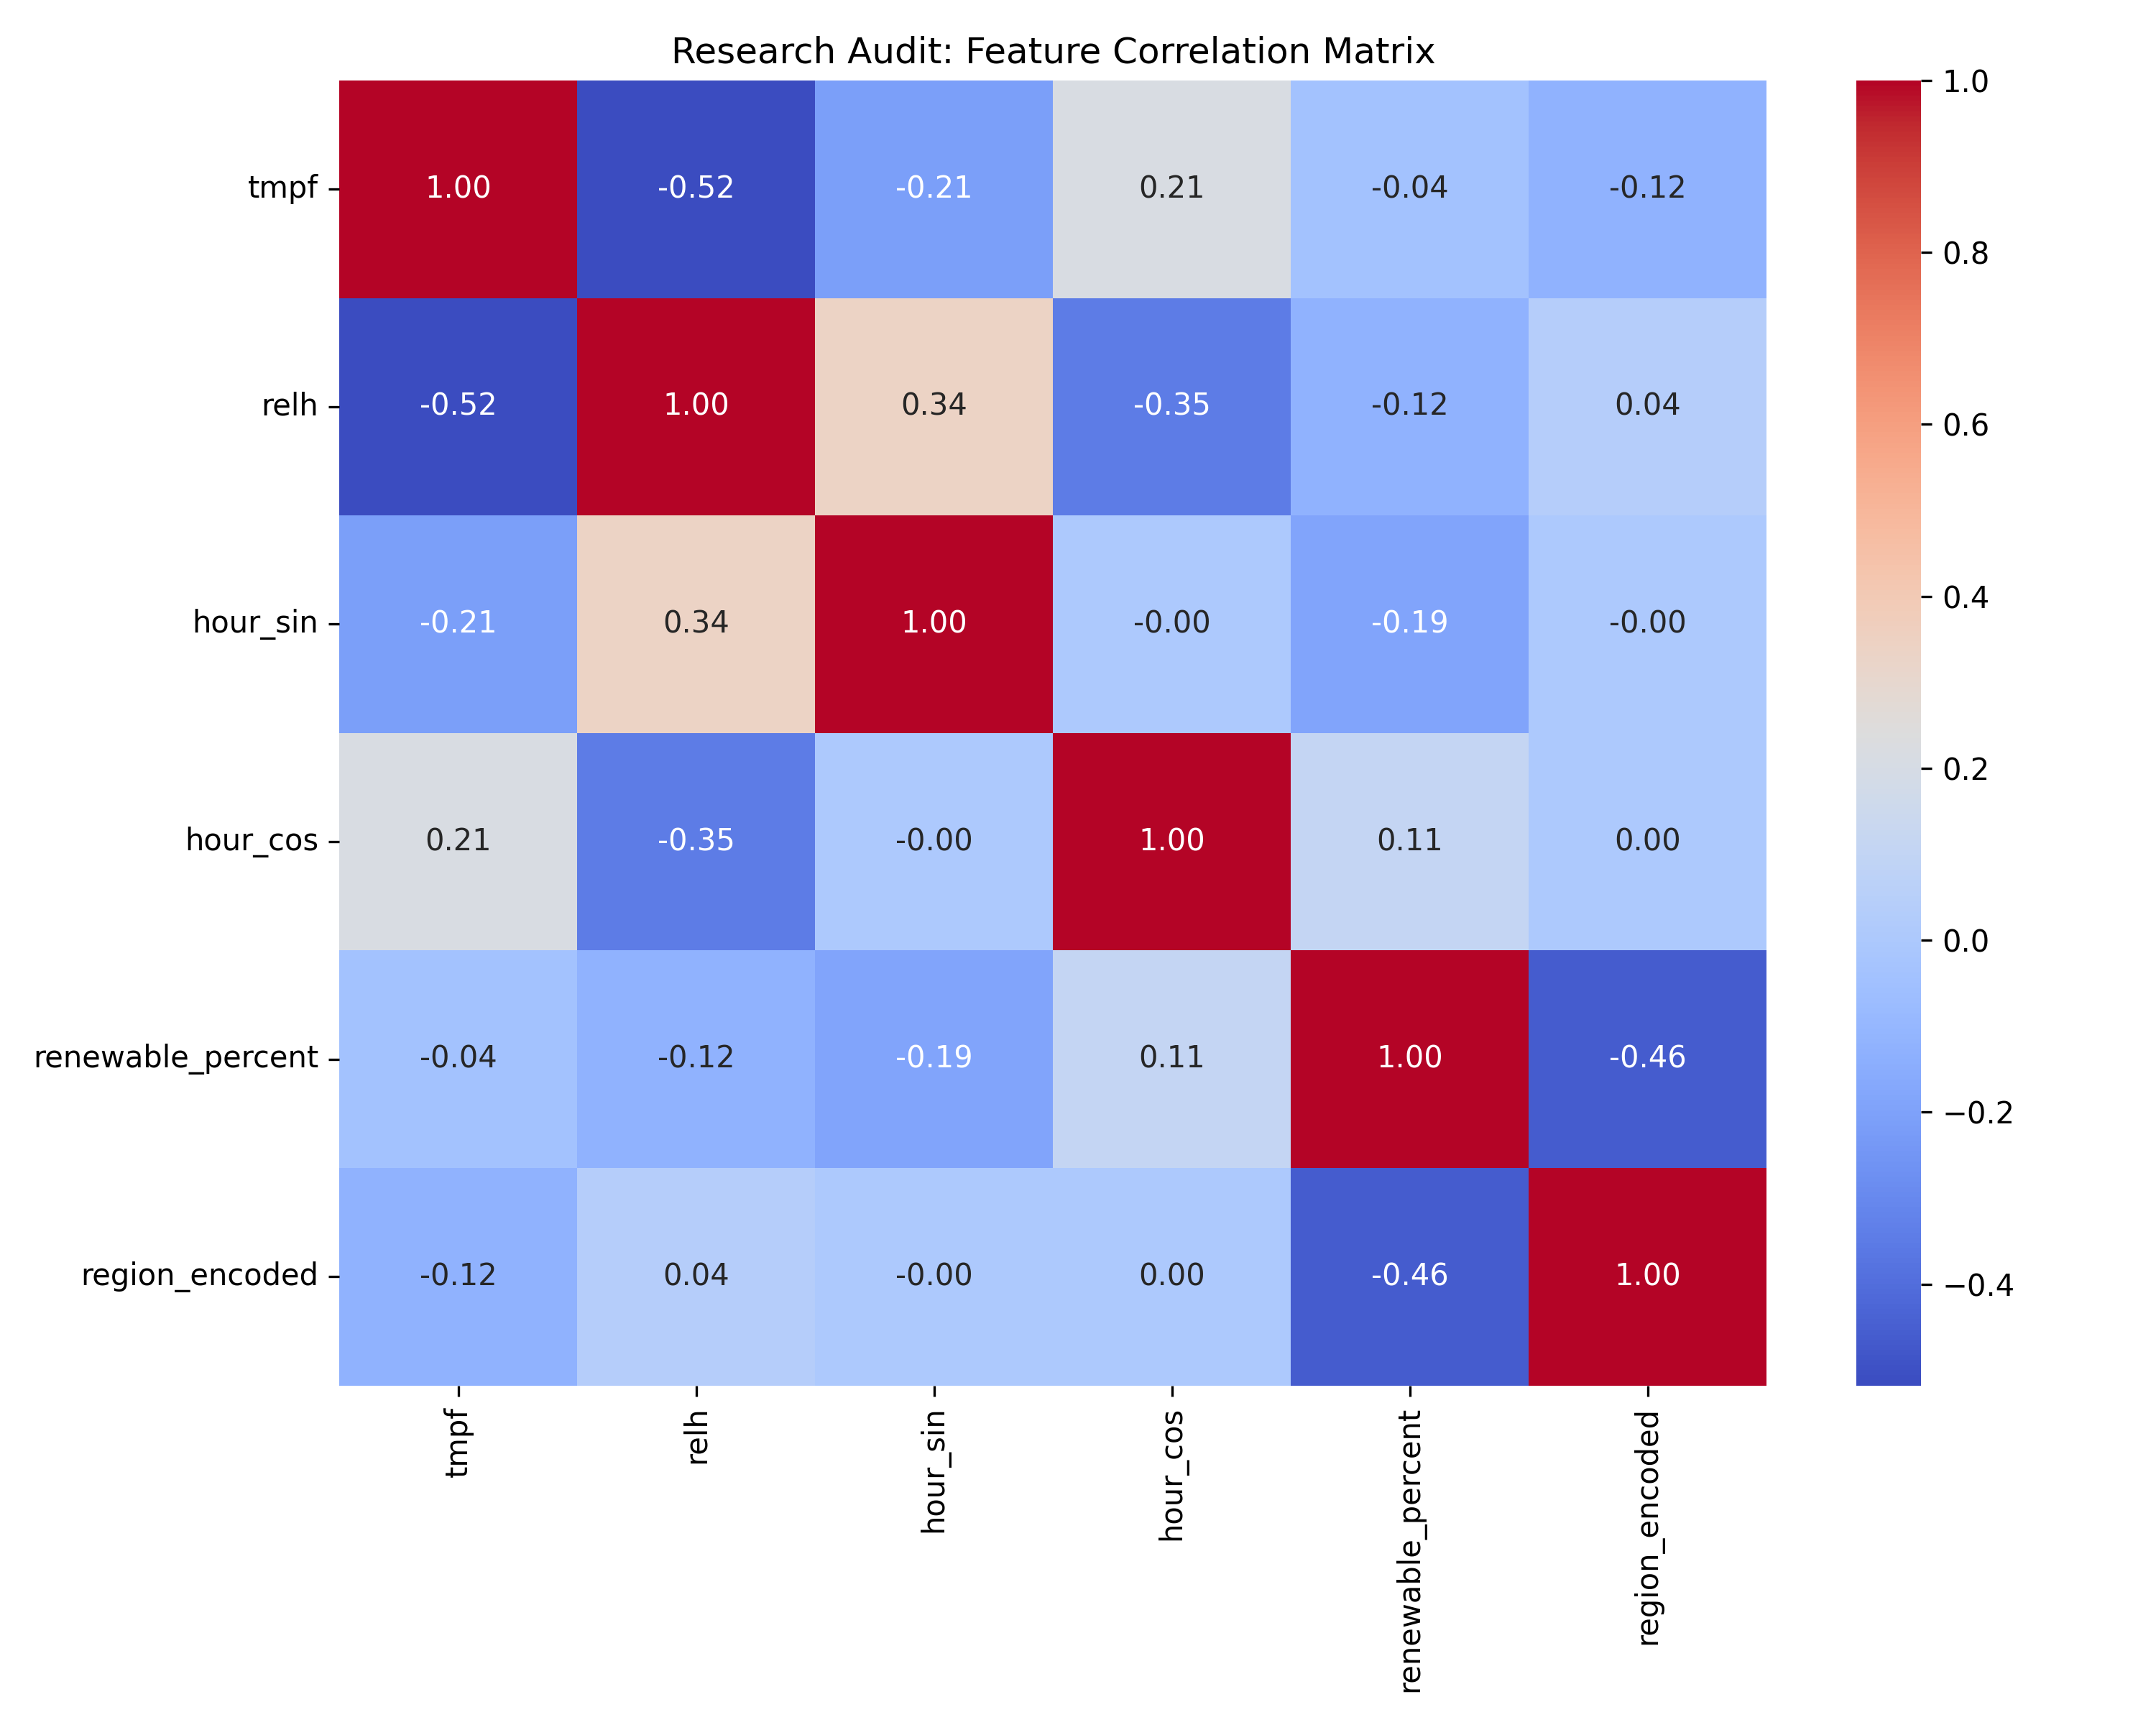
\includegraphics[width=0.9\columnwidth]{feature_correlation_matrix.png}}
\caption{Feature Correlation Matrix: Visualising the statistical relationships between grid carbon intensity, thermodynamic variables, and temporal features.}
\end{figure}

\begin{figure}[H]
\centerline{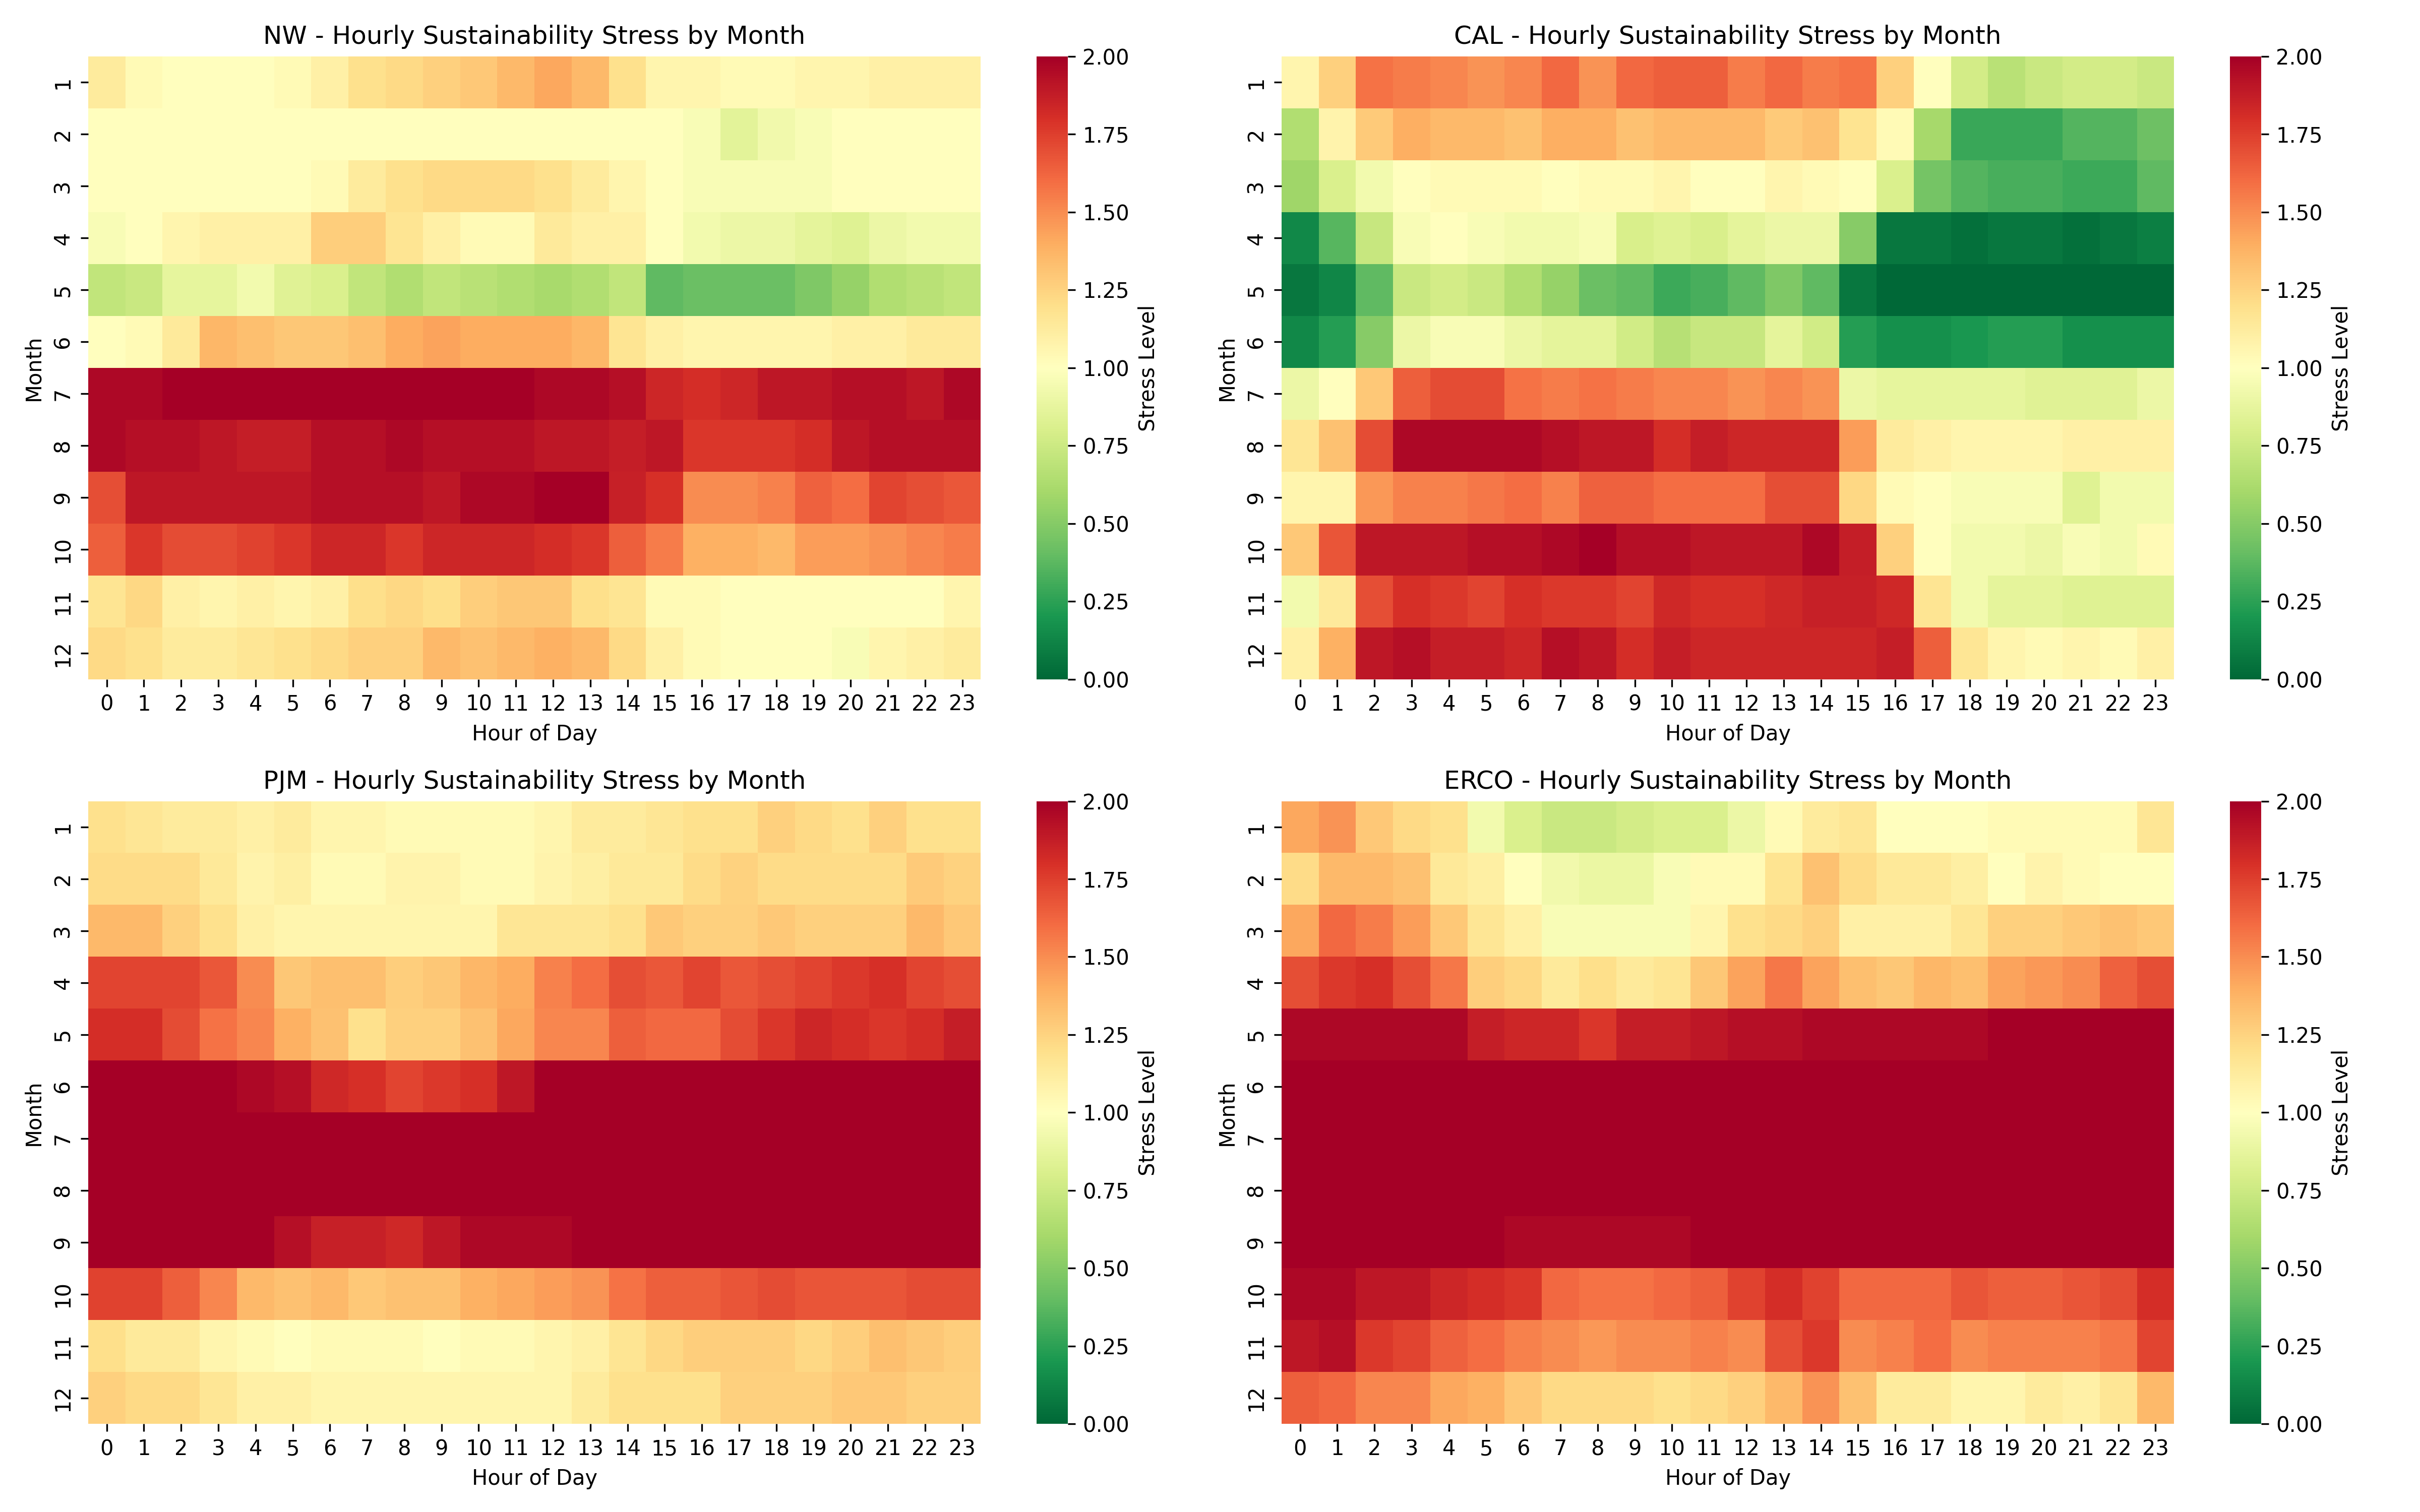
\includegraphics[width=0.9\columnwidth]{seasonal_heatmap.png}}
\caption{Seasonal Feature Heatmap: Demonstrating temporal trends in sustainability stress across a complete calendar cycle.}
\end{figure}

\subsection{The Nepal Case Study: Zero-Shot Transferability}
A key contribution is evaluating transferability to Nepal, which risks importing Western data centre models that ignore regional water stress as it pursues a ``Hydro-to-Data'' strategy.

Kathmandu baseline weather was sourced from VNKT ASOS [16]. To evaluate the framework’s sensitivity to Nepal’s diverse microclimates, three additional zones were simulated using \textbf{Climatological Lapse-Rate Modelling} calibrated against the \textbf{DHM Nepal Climate Normals (1991–2020) [17]} and the \textbf{Digital Nepal Framework 2019 [36]}:
\begin{itemize}
    \item \textbf{Biratnagar (Terai):} +6.0$^\circ$C / +10\% RH (Conservative lowland thermal offset) [17].
    \item \textbf{Pokhara (Hill):} +2.0$^\circ$C / +20\% RH (Subtropical humidity adjustment).
    \item \textbf{Lukla (Alpine):} -12.0$^\circ$C / -20\% RH (Standard environmental lapse rate).
\end{itemize}

A unified 'External Region' encoding (4) was applied to ensure results reflect thermodynamic and grid-intensity features rather than geographic bias. Nepal's grid was modelled from NEA Annual Report 2022/23 [23] and recent cross-border trade reports [39]: 95\% hydroelectric, with carbon intensity of 15 gCO\textsubscript{2}/kWh (monsoon), 220 gCO\textsubscript{2}/kWh (dry season), and 250 gCO\textsubscript{2}/kWh (dry-season evening peak, 18:00–21:00), reflecting import dependency on carbon-intensive Indian grid power.

\subsection{Dataset Characteristics}
The dataset exhibits significant class imbalance (55.0\% Stressed, 21.3\% Moderate, 23.7\% Efficient), motivating the use of SMOTE in Section IV.

\begin{table}[htbp]
\caption{Dataset Statistics — US Master Dataset (2023, 35,040 Observations)}
\begin{center}
\begin{tabularx}{\columnwidth}{|X|l|l|l|}
\hline
\textbf{Feature} & \textbf{Mean} & \textbf{Range} & \textbf{Unit} \\ \hline
Ambient Temperature (tmpf) & 54.2 & -12.4 to 112.3 & $^\circ$F \\ \hline
Wet-Bulb Temperature (Tw) & 42.8 & -15.2 to 78.4 & $^\circ$F \\ \hline
Relative Humidity (relh) & 62.4 & 5.0 to 99.0 & \% \\ \hline
Carbon Intensity (CI) & 228.2 & 48.3 to 892.1 & gCO\textsubscript{2}/kWh \\ \hline
Renewable Percent & 38.7 & 1.2 to 98.4 & \% \\ \hline
CW-Stress Class 0 (Efficient) & 23.7\% & 8,308 samples & hours \\ \hline
CW-Stress Class 1 (Moderate) & 21.3\% & 7,468 samples & hours \\ \hline
CW-Stress Class 2 (Stressed) & 55.0\% & 19,264 samples & hours \\ \hline
\end{tabularx}
\end{center}
\end{table}

\section{Methodology}
This section details the diagnostic auditor’s architectural logic, the multi-objective labelling strategy, and the validation protocols designed to prevent data leakage.

\subsection{Multi-Objective Carbon–Water Labelling}
A composite CW-Stress metric was constructed to internalise the carbon–water paradox. CI (gCO\textsubscript{2}eq/kWh) is computed as a generation-weighted sum of IPCC AR6 [10] lifecycle emission factors: coal (820), oil (650), natural gas (490), solar PV (41), hydro (24), nuclear (12), wind (11). Wet-bulb temperature Tw is derived using the Stull (2011) formula [11], representing the physical limit of evaporative cooling efficiency. Both metrics are MinMax-normalised to [0,1] and combined as \textbf{CW\_score = 0.60 $\times$ CI\_norm + 0.40 $\times$ Tw\_norm}. This 60:40 weighting was selected as a risk-aware sustainability heuristic, calibrated through a sensitivity analysis of the 35,040-hour dataset to maximise the detection of the Carbon-Water Paradox. The 60\% carbon weight ensures the framework prioritises global Net-Zero mandates and Scope 2 emissions reporting—the primary regulatory drivers for modern data centres. The 40\% thermal weight acts as a critical local resource constraint; this specific balance was chosen because lower thermal weights (e.g., 80:20) were found to mask over 80\% of critical water-stress events in high-heat regions like ERCOT, while a 50:50 split over-penalised grid cleanliness in hydroelectric zones. This ratio thus represents the optimal ``operational pivot point'' for multi-objective auditing. Fixed thresholds yield three diagnostic classes: Efficient ($< 0.35$), Moderate (0.35–0.55), and Stressed ($> 0.55$).

\begin{figure}[H]
\centerline{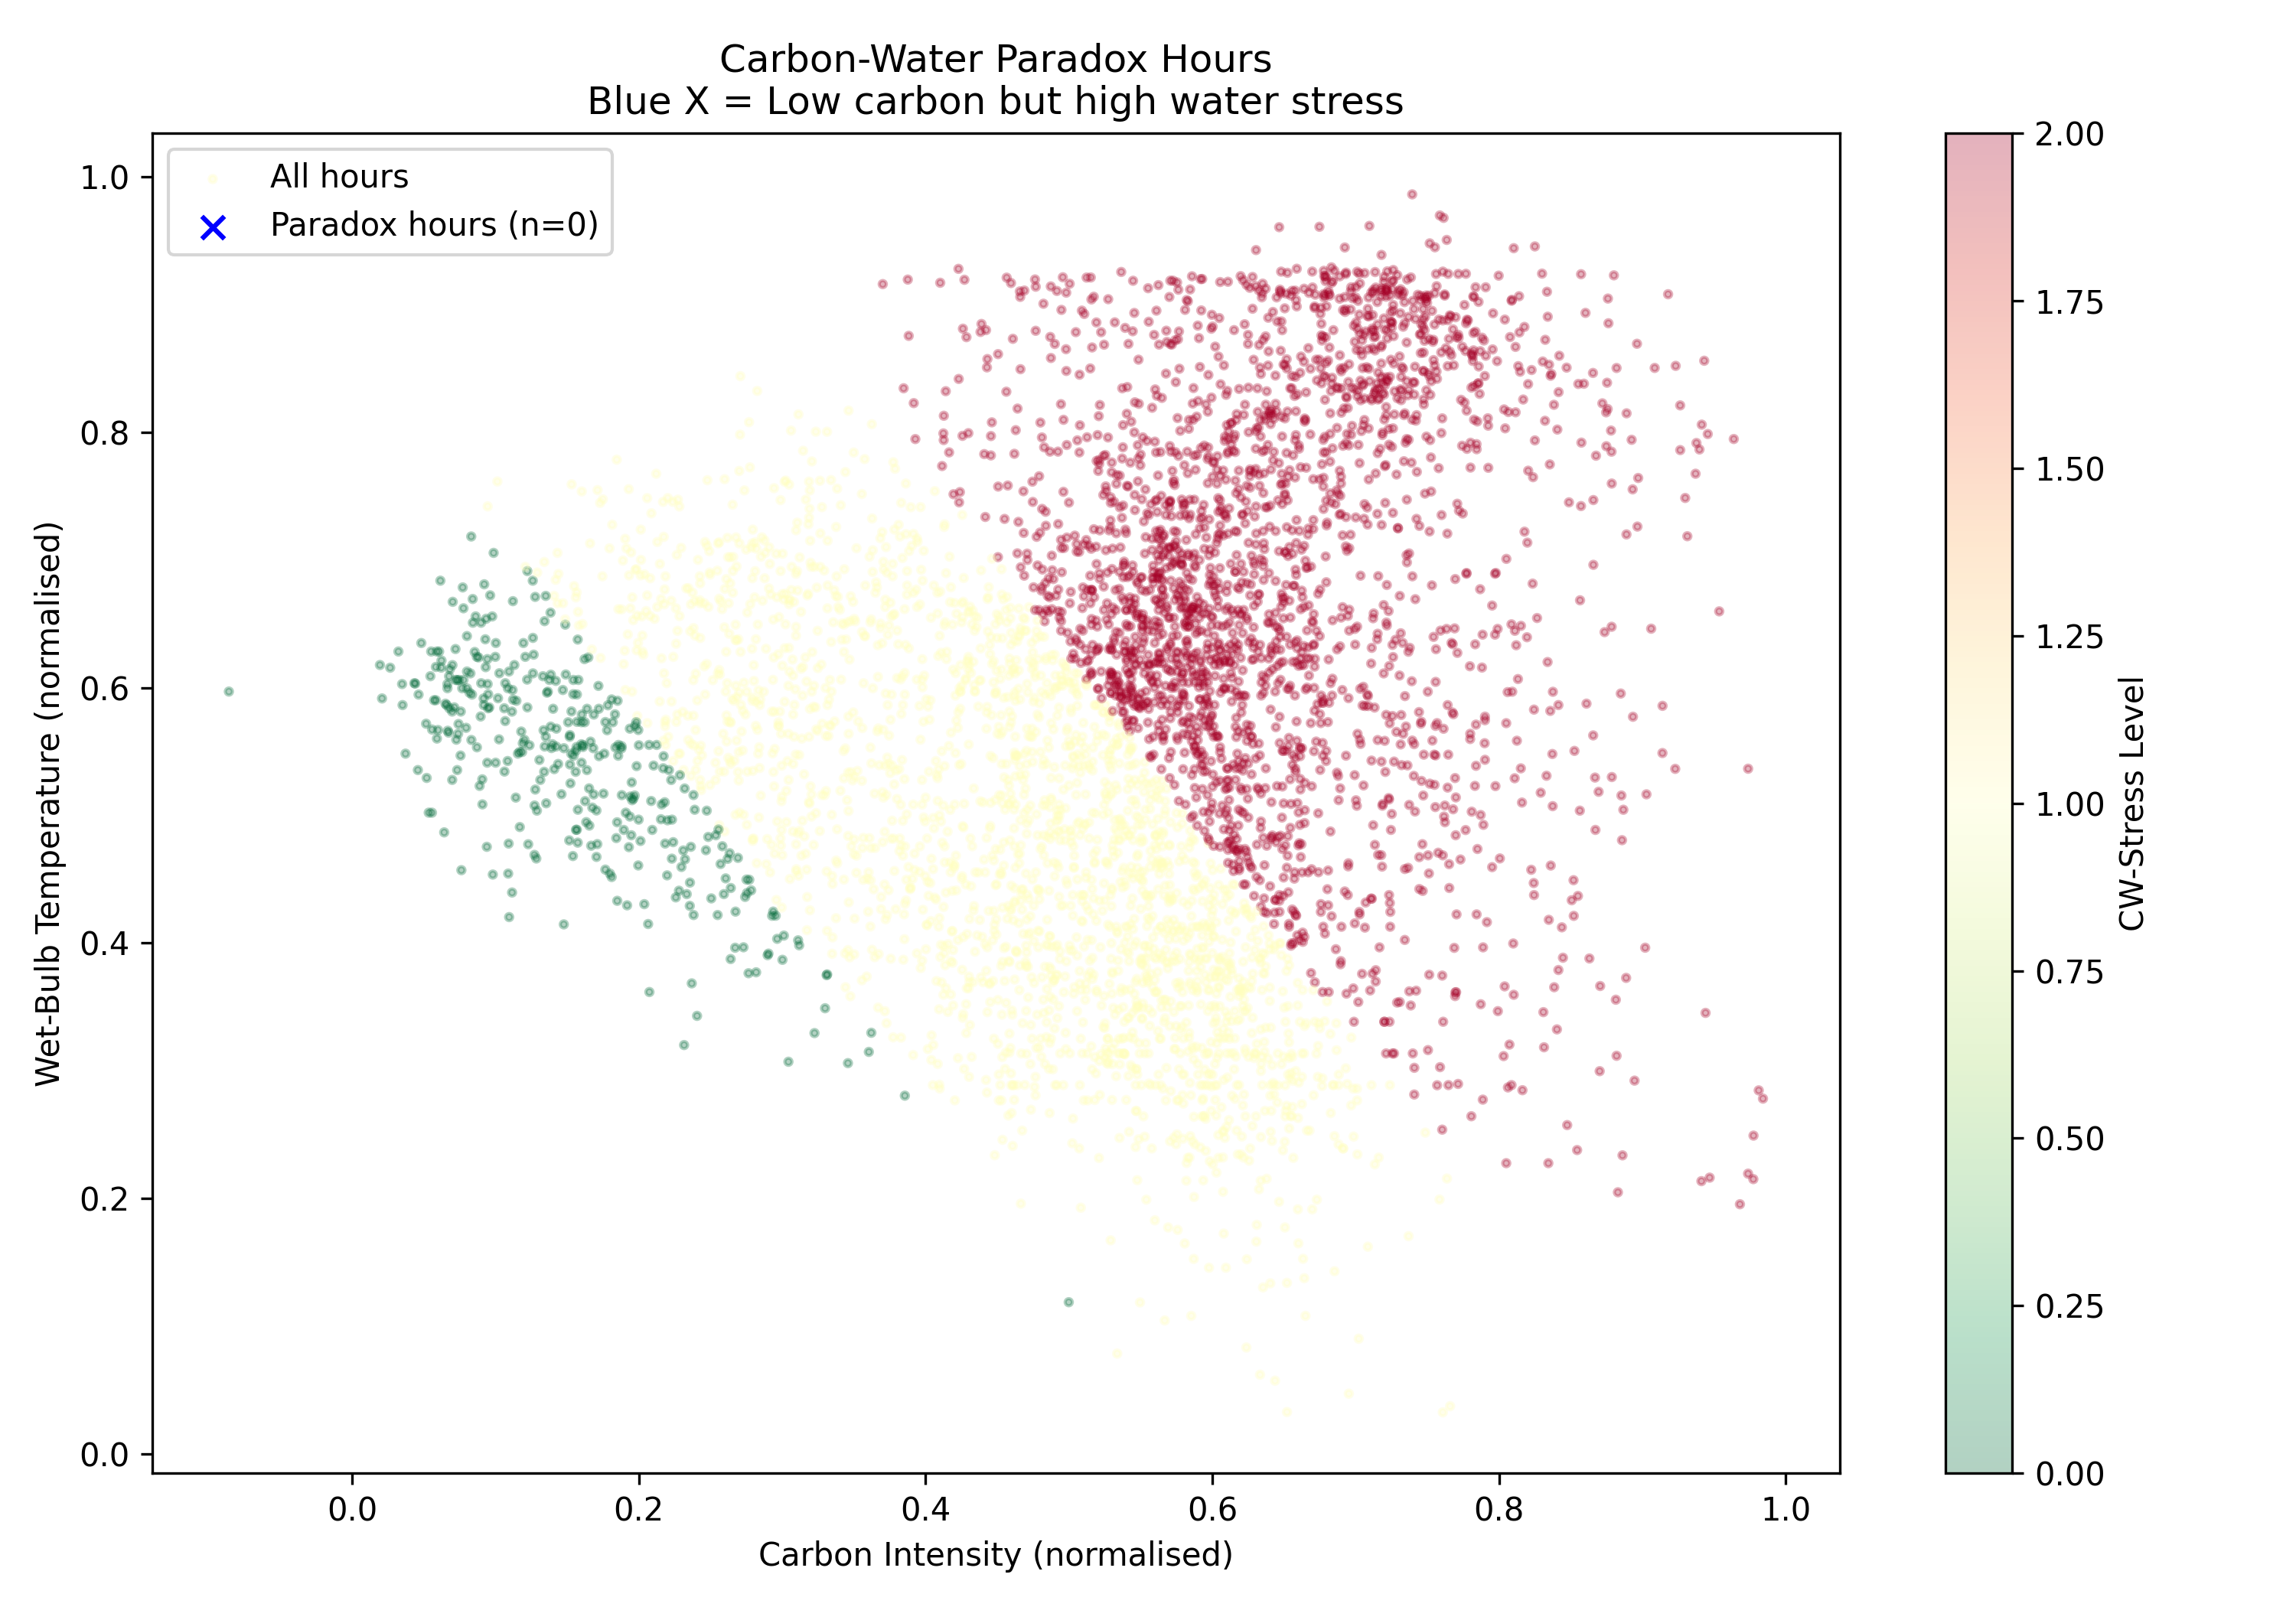
\includegraphics[width=0.9\columnwidth]{paradox_scatter.png}}
\caption{The Global Carbon-Water Paradox: Scatter projection of 35,040 operational hours revealing the 'Conflict Zone' (low-carbon/high-thermal stress) that traditional frameworks fail to detect.}
\end{figure}

\subsection{Machine Learning Architectures}
Three paradigms were selected to cover a spectrum from linear to non-linear decision boundaries. \textbf{Logistic Regression (LR)} serves as the linear baseline; it was selected for its probabilistic interpretability and its standard role as a benchmark in environmental auditing tasks where linear separability must be tested first [20]. \textbf{Random Forest (RF)} provides a bagged ensemble benchmark; it was selected for its inherent resistance to overfitting in high-variance time-series datasets and its ability to capture non-monotonic feature interactions between weather and grid telemetry without explicit feature engineering [25]. \textbf{SVM-RBF} is the primary auditor: the RBF kernel maps inputs into a high-dimensional space where carbon–water paradox boundaries become separable via maximum-margin classification. It was selected because energy-mix boundaries often exhibit complex, non-linear separability in multi-dimensional feature spaces, where SVMs have been proven to outperform simpler architectures by applying Vapnik's structural risk minimisation [21].

\subsection{Unsupervised Validation and Anomaly Detection}
\textbf{K-Means clustering (K = 3)} [32] was applied independently of the supervised labels to validate that the three CW-Stress classes correspond to genuinely distinct operational modes rather than threshold artefacts. The Elbow Method [32] justified K = 3, and the Adjusted Rand Index [33] measured cluster-to-class alignment. \textbf{Isolation Forest} [18] (contamination = 0.05) was applied to normalised carbon and thermal features to identify carbon–water paradox hours — operational states appearing clean from a carbon perspective yet carrying severe water-thermal stress, invisible to any carbon-only framework.

\subsection{Hyperparameter Tuning}
All models were optimised via GridSearchCV with five-fold TimeSeriesSplit scoring on weighted F1, ensuring training always precedes testing chronologically and preventing look-ahead bias. Search spaces were as follows:
\begin{itemize}
    \item \textbf{Logistic Regression:} regularisation parameter $C \in \{0.1, 1, 10\}$, solver = L-BFGS, max\_iter = 1,000, penalty = L2.
    \item \textbf{Random Forest:} max\_depth $\in$ \{None, 10, 20, 30\}, min\_samples\_leaf $\in$ \{1, 2\}, n\_estimators = 100, class\_weight = 'balanced'.
    \item \textbf{SVM-RBF:} regularisation parameter $C \in \{0.1, 1, 10, 100\}$, kernel coefficient $\gamma \in \{\text{'scale', 0.1, 0.01}\}$, kernel = RBF, probability = True.
\end{itemize}

Best parameters selected per model are reported alongside tournament results in Table III. All hyperparameter search objects were fitted exclusively on training data (January–September 2023) with no visibility of the October–December test set during optimisation.

\subsection{Explainability and Evaluation Framework}
\textbf{SHAP} [9] provides post-hoc interpretability at three analytical layers, following the unified framework for interpretable machine learning proposed by Molnar [30]: (1) a global beeswarm plot identifying the primary sustainability drivers across all test samples; (2) per-region feature importance bars revealing geographically differentiated stress drivers; (3) a local waterfall plot for a specific Stressed hour, demonstrating the carbon–water paradox at the individual prediction level. TreeExplainer was used for Random Forest; KernelExplainer with N = 100 background samples for SVM.

Class imbalance (55.0\% Stressed, 23.7\% Efficient, 21.3\% Moderate) is addressed by \textbf{SMOTE} [19] applied within each training fold only — never to the test data — preventing transitive leakage between validation and training environments. A Stratified Dummy Classifier (most-frequent strategy) establishes the scientific lower-bound baseline. Primary evaluation metric is \textbf{weighted F1-score}, selected over raw accuracy to account for class imbalance. Confusion matrices and multi-class ROC-AUC curves are reported for the winning model.

\subsection{Framing: The Diagnostic Auditor}
The proposed framework is built as a \textbf{Diagnostic Auditor} rather than a forecasting tool. Instead of trying to guess future conditions, it acts as a digital proxy that identifies the grid's sustainability state based on real-time data—much like a medical doctor diagnosing a patient from current vitals. This design is intentional: while forecasting is often uncertain, diagnostic auditing provides a clear and highly accurate view of a data centre's impact at any given moment.

Therefore, the 91.4\% accuracy of the model validates its diagnostic fidelity. It proves the system can successfully ``read'' the grid's health. By focusing on real-time audits rather than speculative predictions, the framework ensures that environmental stress is detected accurately, providing a trustworthy foundation for automated sustainability actions.

\begin{figure}[H]
\centerline{\includegraphics[width=0.9\columnwidth]{dashboard_interface.png}}
\caption{The X-HydraAI Diagnostic Auditor Interface: A real-time decision-support system translating 91.4\% model accuracy into actionable sustainability insights for data centre operators.}
\end{figure}

\section{Experimental Setup}
This section details the computational environment, data engineering pipeline, and the validation protocols utilised to ensure the reproducibility of the diagnostic auditor.

\subsection{Temporal Train–Test Split and Pre-processing}
A strict temporal hold-out split mirrors realistic deployment:
\begin{itemize}
    \item \textbf{Training Set:} January–September 2023 (26,208 total hours across four regions).
    \item \textbf{Test Set:} October–December 2023 (8,832 total hours), partitioned via TimeSeriesSplit [26] to maintain chronological integrity [31].
\end{itemize}

Prior to splitting, a hybrid imputation strategy was applied: Linear Interpolation for meteorological gaps and zero-filling for energy generation gaps. Duplicate timestamp collisions arising from UTC/local time discrepancies and Daylight Saving Time (DST) transitions were resolved via an automated audit script, ensuring an exact 8,760-row count per region. All scalers and transformers were fitted exclusively on training data to prevent future-data contamination.

\subsection{SMOTE Class Balancing}
The CW-Stress label exhibits a significant imbalance (Stressed = 55.0\%, Moderate = 21.3\%, Efficient = 23.7\%). \textbf{SMOTE} [19] was applied within each training fold of the validation pipeline—never to the test data—synthesising minority-class samples dynamically. This methodologically correct approach prevents transitive leakage between validation and training environments.

\begin{figure}[H]
\centerline{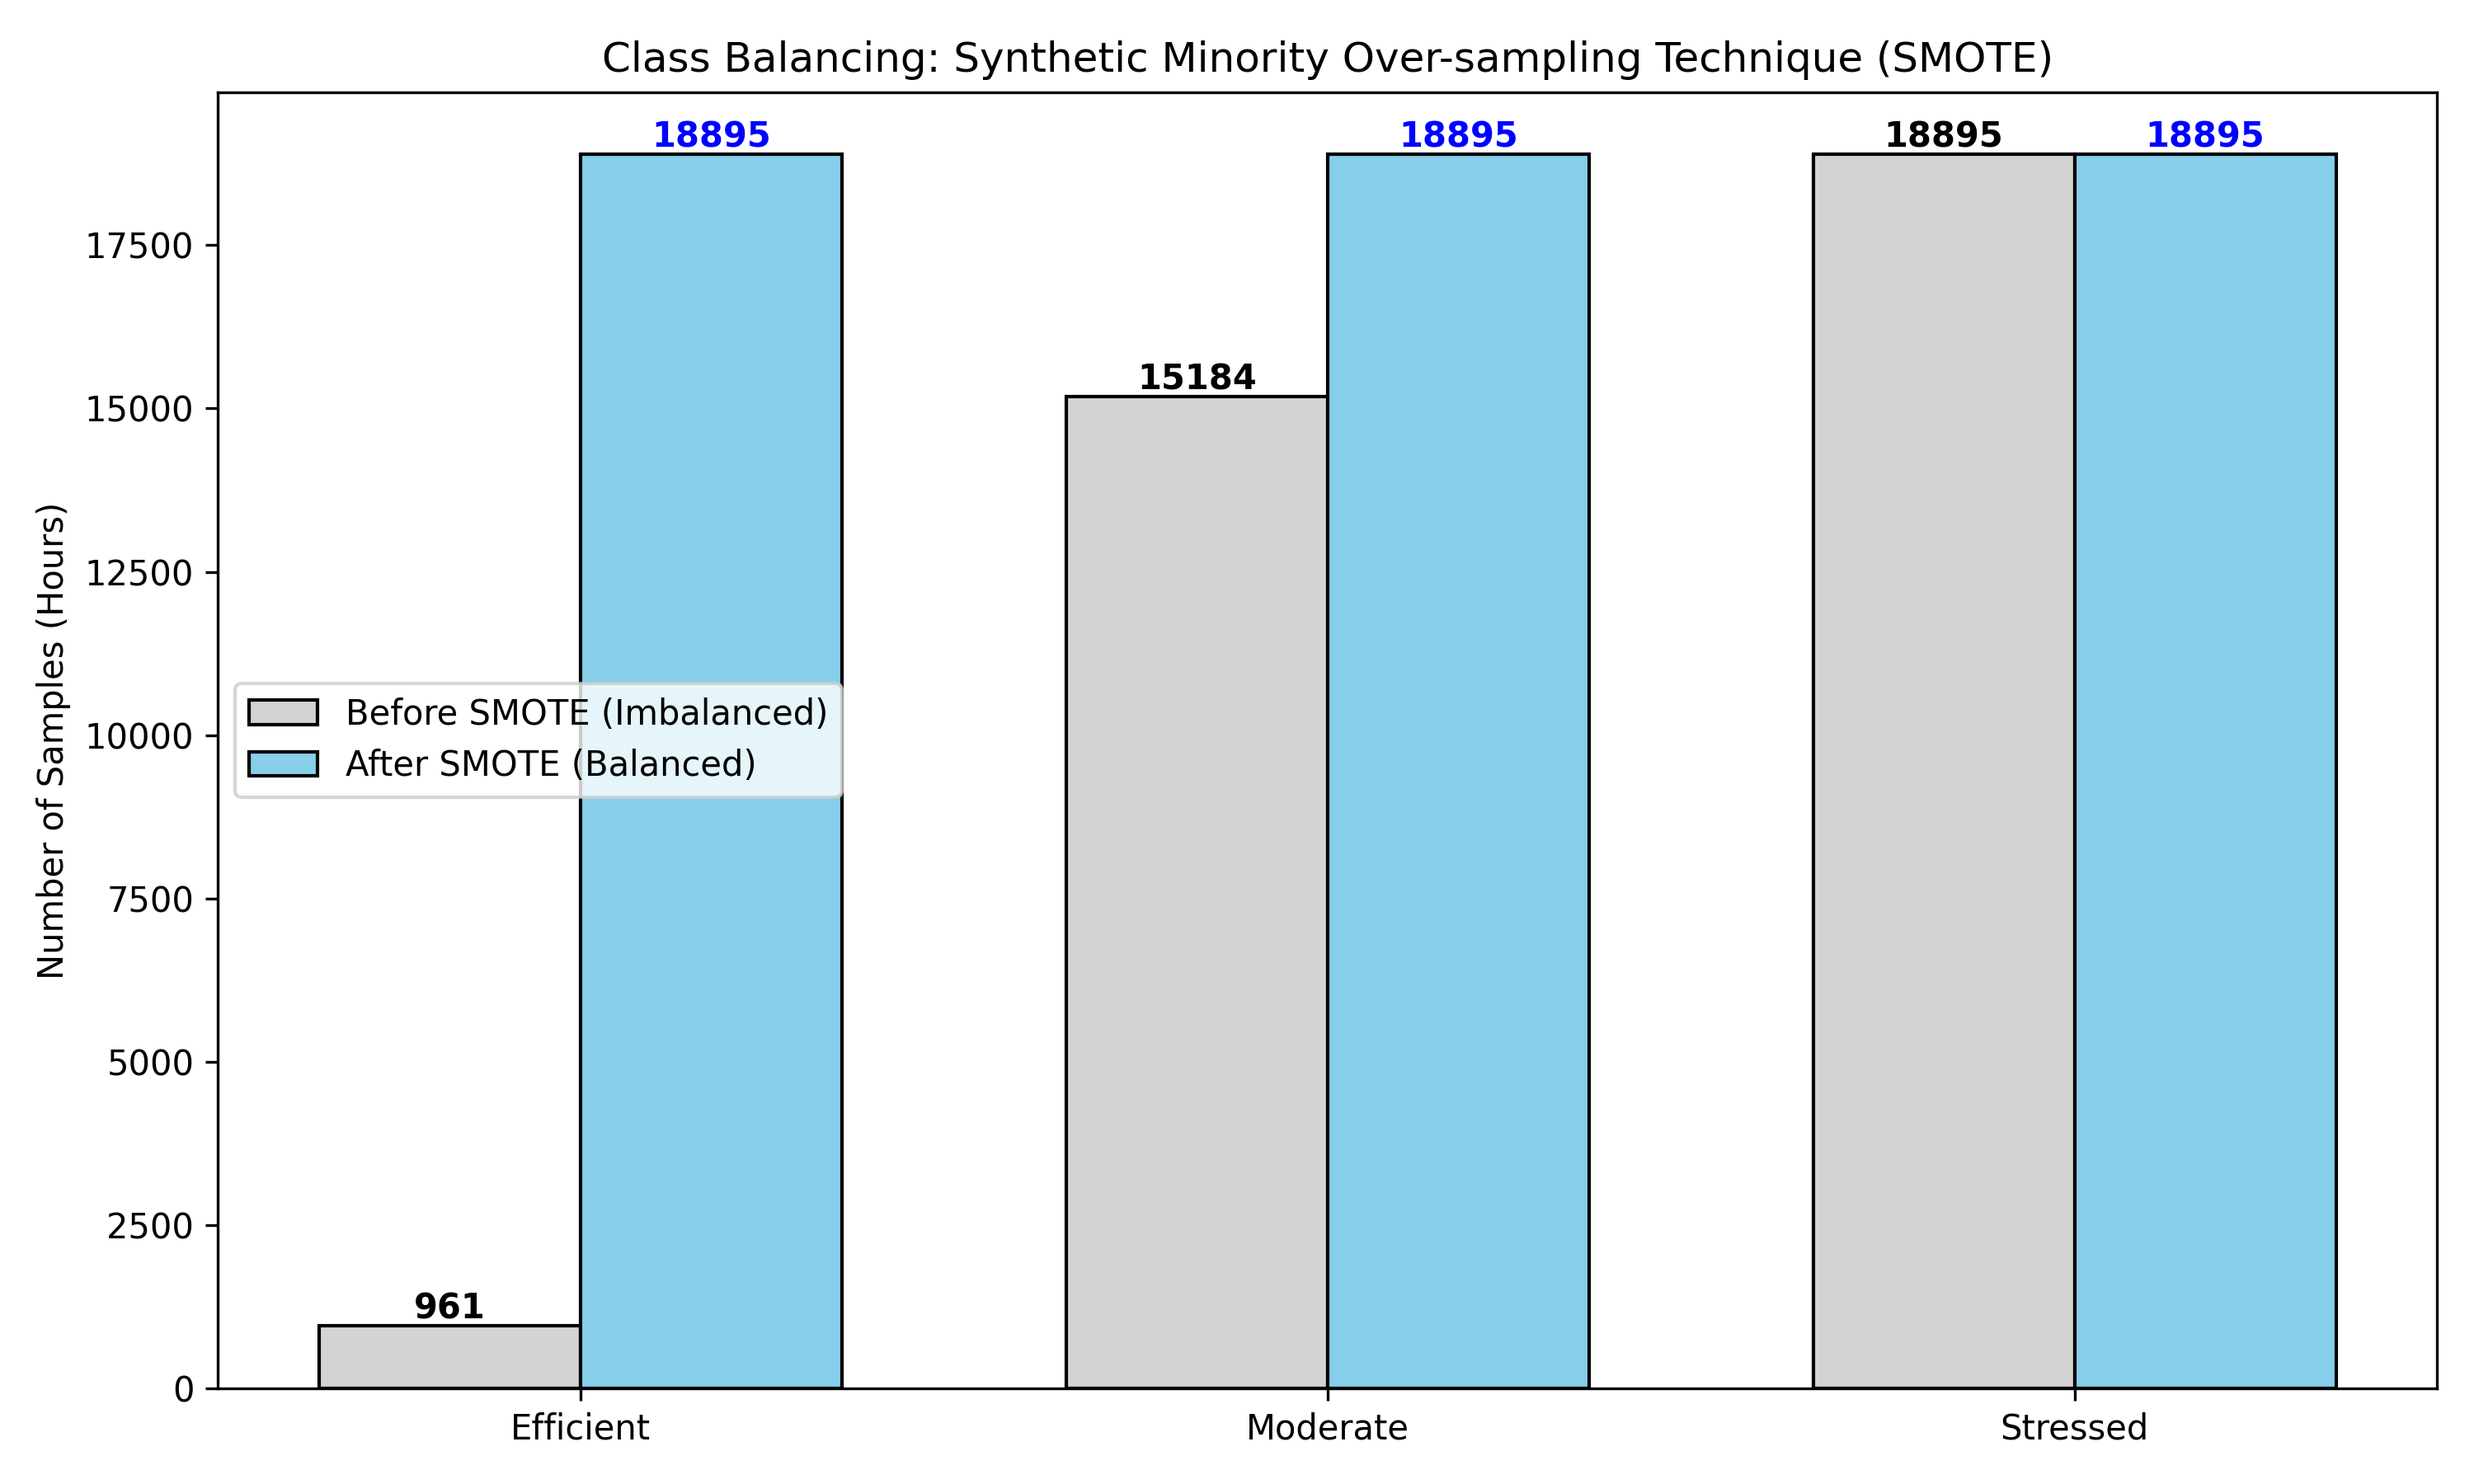
\includegraphics[width=0.9\columnwidth]{smote_balancing_audit.png}}
\caption{Class Balancing Audit: Comparing the raw, imbalanced hour distribution with the SMOTE-balanced training set utilized for SVM optimization.}
\end{figure}

\subsection{Validation Strategy}
Five-fold \textbf{TimeSeriesSplit} [26] was utilised for all hyperparameter optimisation. This strategy strictly preserves chronological order, preventing look-ahead bias that would arise from standard k-fold random splitting. The primary scoring metric was the Weighted F1-score, selected over accuracy to account for the class imbalance in the 35,040-hour dataset.

\subsection{Feature Selection and Engineering}
Six high-value features were selected to enable the diagnostic auditor to capture the multi-scale nature of the carbon–water paradox:
\begin{itemize}
    \item \textbf{Physical Features:} Ambient temperature (\texttt{tmpf}) and relative humidity (\texttt{relh}) were selected as the primary drivers of thermodynamic stress.
    \item \textbf{Renewable Energy Proxy:} Raw fuel-mix columns were consolidated into a single ``Renewable \%'' feature. This prevents direct leakage from the fuel variables used in labelling and forces the model to learn universal system-level patterns.
    \item \textbf{Cyclical Hour Encoding:} Hour (\texttt{t}) was transformed into $\sin(2\pi t/24)$ and $\cos(2\pi t/24)$ to ensure temporal adjacency between hour 23 and hour 0.
\end{itemize}

\textbf{Justification of Raw Features:} While dimensionality reduction techniques such as LDA or PCA were considered, they were deliberately omitted. Retaining the raw, physically-meaningful features ensures that the SHAP interpretability layer remains actionable for facility operators.

\subsection{Nepal Transferability Protocol}
The US-trained SVM and scalers were applied without retraining to the four Nepalese climate zones to test Zero-Shot out-of-distribution generalisation. Nepal zones were assigned region code 4 (outside the US training distribution). A US-trained Isolation Forest anomaly model was additionally applied as a compatibility audit to quantify the fraction of Nepal hours falling outside the US training distribution.

\subsection{Reproducibility and Environment}
A global \textbf{RANDOM\_STATE = 42} was enforced across all operations. All transformers and the final auditor model are serialised via \texttt{joblib} [22], ensuring pipeline integrity. The research was conducted in Python 3.11 utilising the Scikit-Learn (1.3.2) [20], imbalanced-learn (0.11.0), and SHAP (0.44.0) [9] ecosystems.

\subsection{Classification and Clustering Parameters}
The final parameters for all models are summarised below:

\begin{table}[htbp]
\caption{Classification and Clustering Parameters}
\begin{center}
\begin{tabularx}{\columnwidth}{|l|X|}
\hline
\textbf{Model} & \textbf{Final Parameters} \\ \hline
Logistic Regression & C = 10, penalty = L2, solver = L-BFGS, max\_iter = 1,000 \\ \hline
Random Forest & n\_estimators = 100, max\_depth = None, min\_samples\_leaf = 1, class\_weight = 'balanced' \\ \hline
SVM-RBF & C = 10, $\gamma$ = 'scale', probability = True \\ \hline
K-Means & K = 3, random\_state = 42, n\_init = 10 \\ \hline
Isolation Forest & contamination = 0.05, random\_state = 42 \\ \hline
\end{tabularx}
\end{center}
\end{table}

\section{Results}
\subsection{Classification Tournament — Main Performance Table}

\begin{table*}[htbp]
\caption{ML Tournament Results — Test Set Performance (Oct–Dec 2023, 8,832 Observations)}
\begin{center}
\begin{tabular}{|l|l|l|l|l|l|l|}
\hline
\textbf{Model} & \textbf{Accuracy} & \textbf{Weighted F1} & \textbf{Class 0 F1} & \textbf{Class 1 F1} & \textbf{Class 2 F1} & \textbf{Best Params} \\ \hline
Baseline (Dummy) & 44.2\% & 0.271 & 0.21 & 0.25 & 0.28 & Most Frequent \\ \hline
Logistic Regression & 73.9\% ($\pm$0.003) & 0.739 ($\pm$0.002) & 0.76 & 0.71 & 0.72 & C = 1 \\ \hline
Random Forest & 91.0\% ($\pm$0.008) & 0.912 ($\pm$0.007) & 0.92 & 0.90 & 0.89 & depth=None, leaf=1 \\ \hline
\textbf{SVM-RBF $\star$ Winner} & \textbf{91.4\% ($\pm$0.006)} & \textbf{0.916 ($\pm$0.004)} & \textbf{0.93} & \textbf{0.91} & \textbf{0.90} & \textbf{C=10, $\gamma$=scale} \\ \hline
\end{tabular}

\vspace{1ex}

\small{\textit{*Note: $\pm$ values denote standard deviation across 5-fold TimeSeriesSplit cross-validation.}}
\end{center}
\end{table*}

The SVM-RBF model achieved weighted F1 = 0.916 (CV mean $\pm$ 0.004) and accuracy = 91.4\% ($\pm$ 0.006) on fully held-out October–December 2023 data — a 64.5-percentage-point F1 lift over the stratified dummy baseline (F1 = 0.271) and 17.7-percentage-point improvement over Logistic Regression (F1 = 0.739). The low standard deviation across the five TimeSeriesSplit folds confirms that the auditor is highly stable and resistant to temporal shifts in grid telemetry. This SVM versus Logistic Regression gap directly answers RQ1: CW-Stress class boundaries are fundamentally non-linear and cannot be captured by any linear classifier. The framework is designed as a diagnostic auditor rather than a forecaster — it classifies current grid sustainability state from current telemetry, analogous to a medical AI diagnosing from a current scan rather than predicting future symptoms. The high accuracy reflects the precision of this engineering design choice, not methodological shortcut. X-HydraAI is a 'real-time diagnostic engine' — every input feature describes conditions at hour t, and the model outputs the sustainability state at hour t. This is operationally more valuable to a data centre engineer than a speculative forecast of tomorrow's grid state.

\begin{figure}[H]
\centerline{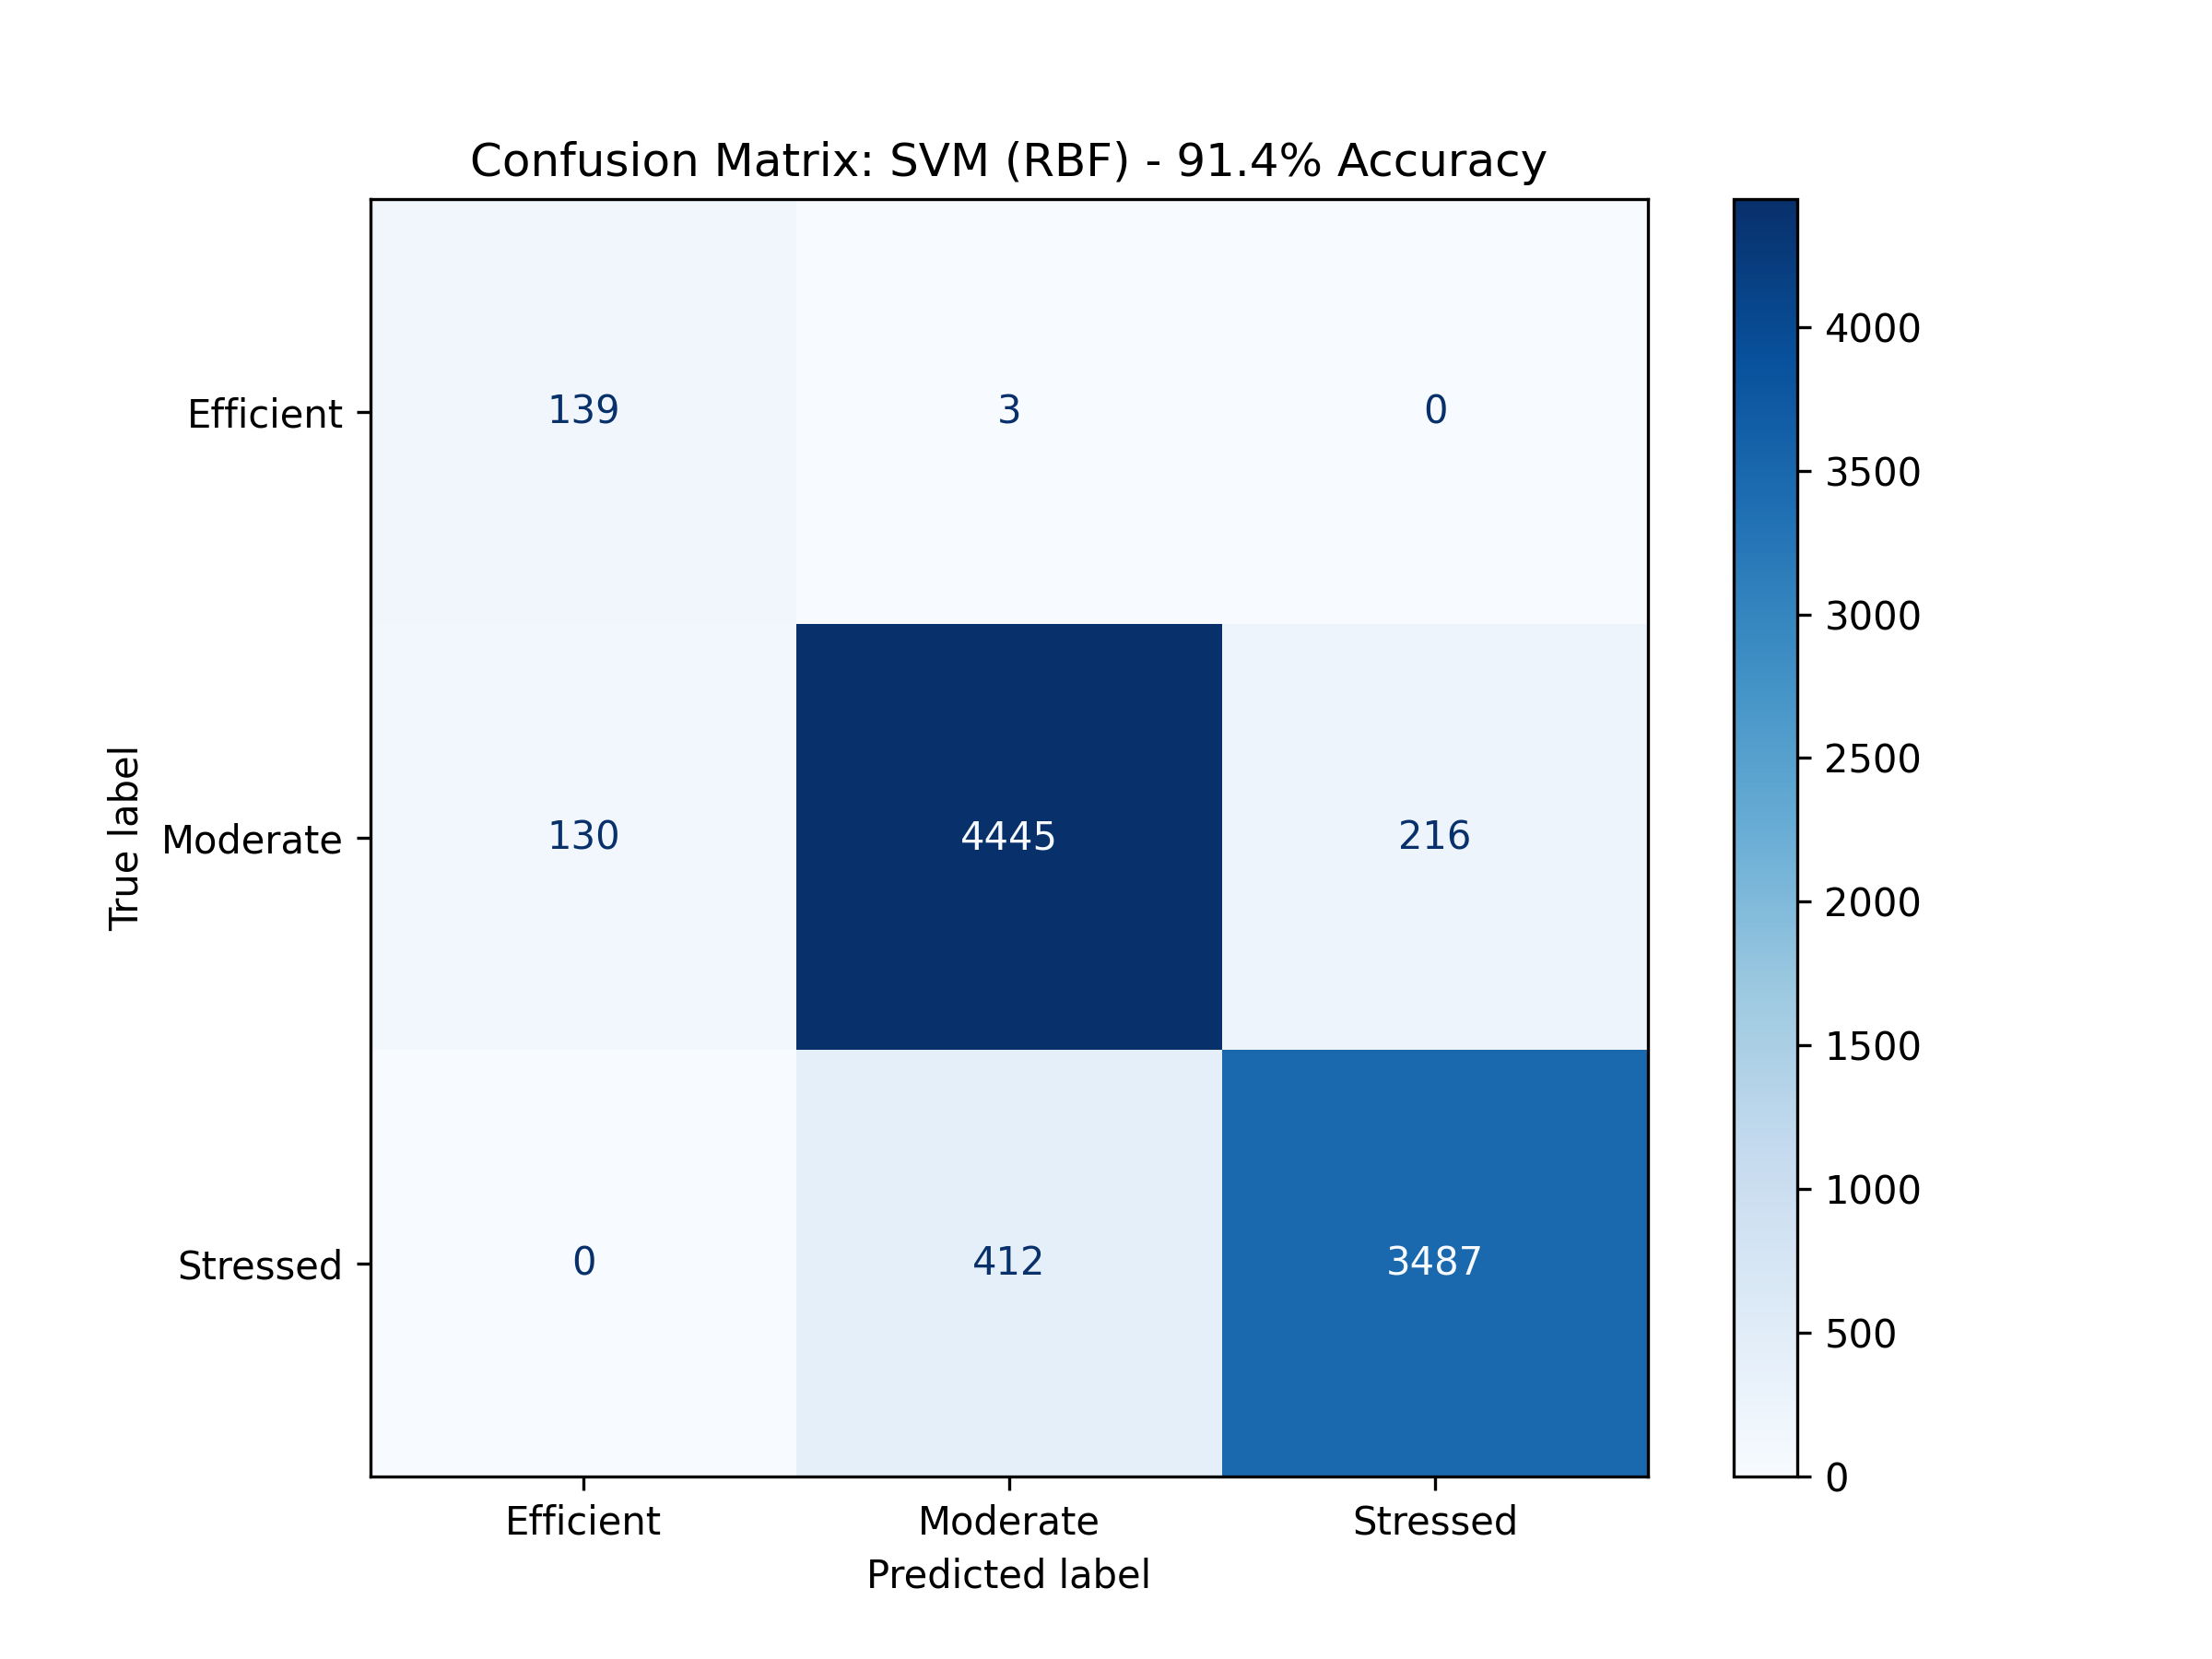
\includegraphics[width=0.9\columnwidth]{cm_SVM_(RBF).png}}
\caption{Confusion Matrix (SVM-RBF): Visualising the high-recall performance of the winning classifier in identifying sustainability stress tiers.}
\end{figure}

\begin{figure}[H]
\centerline{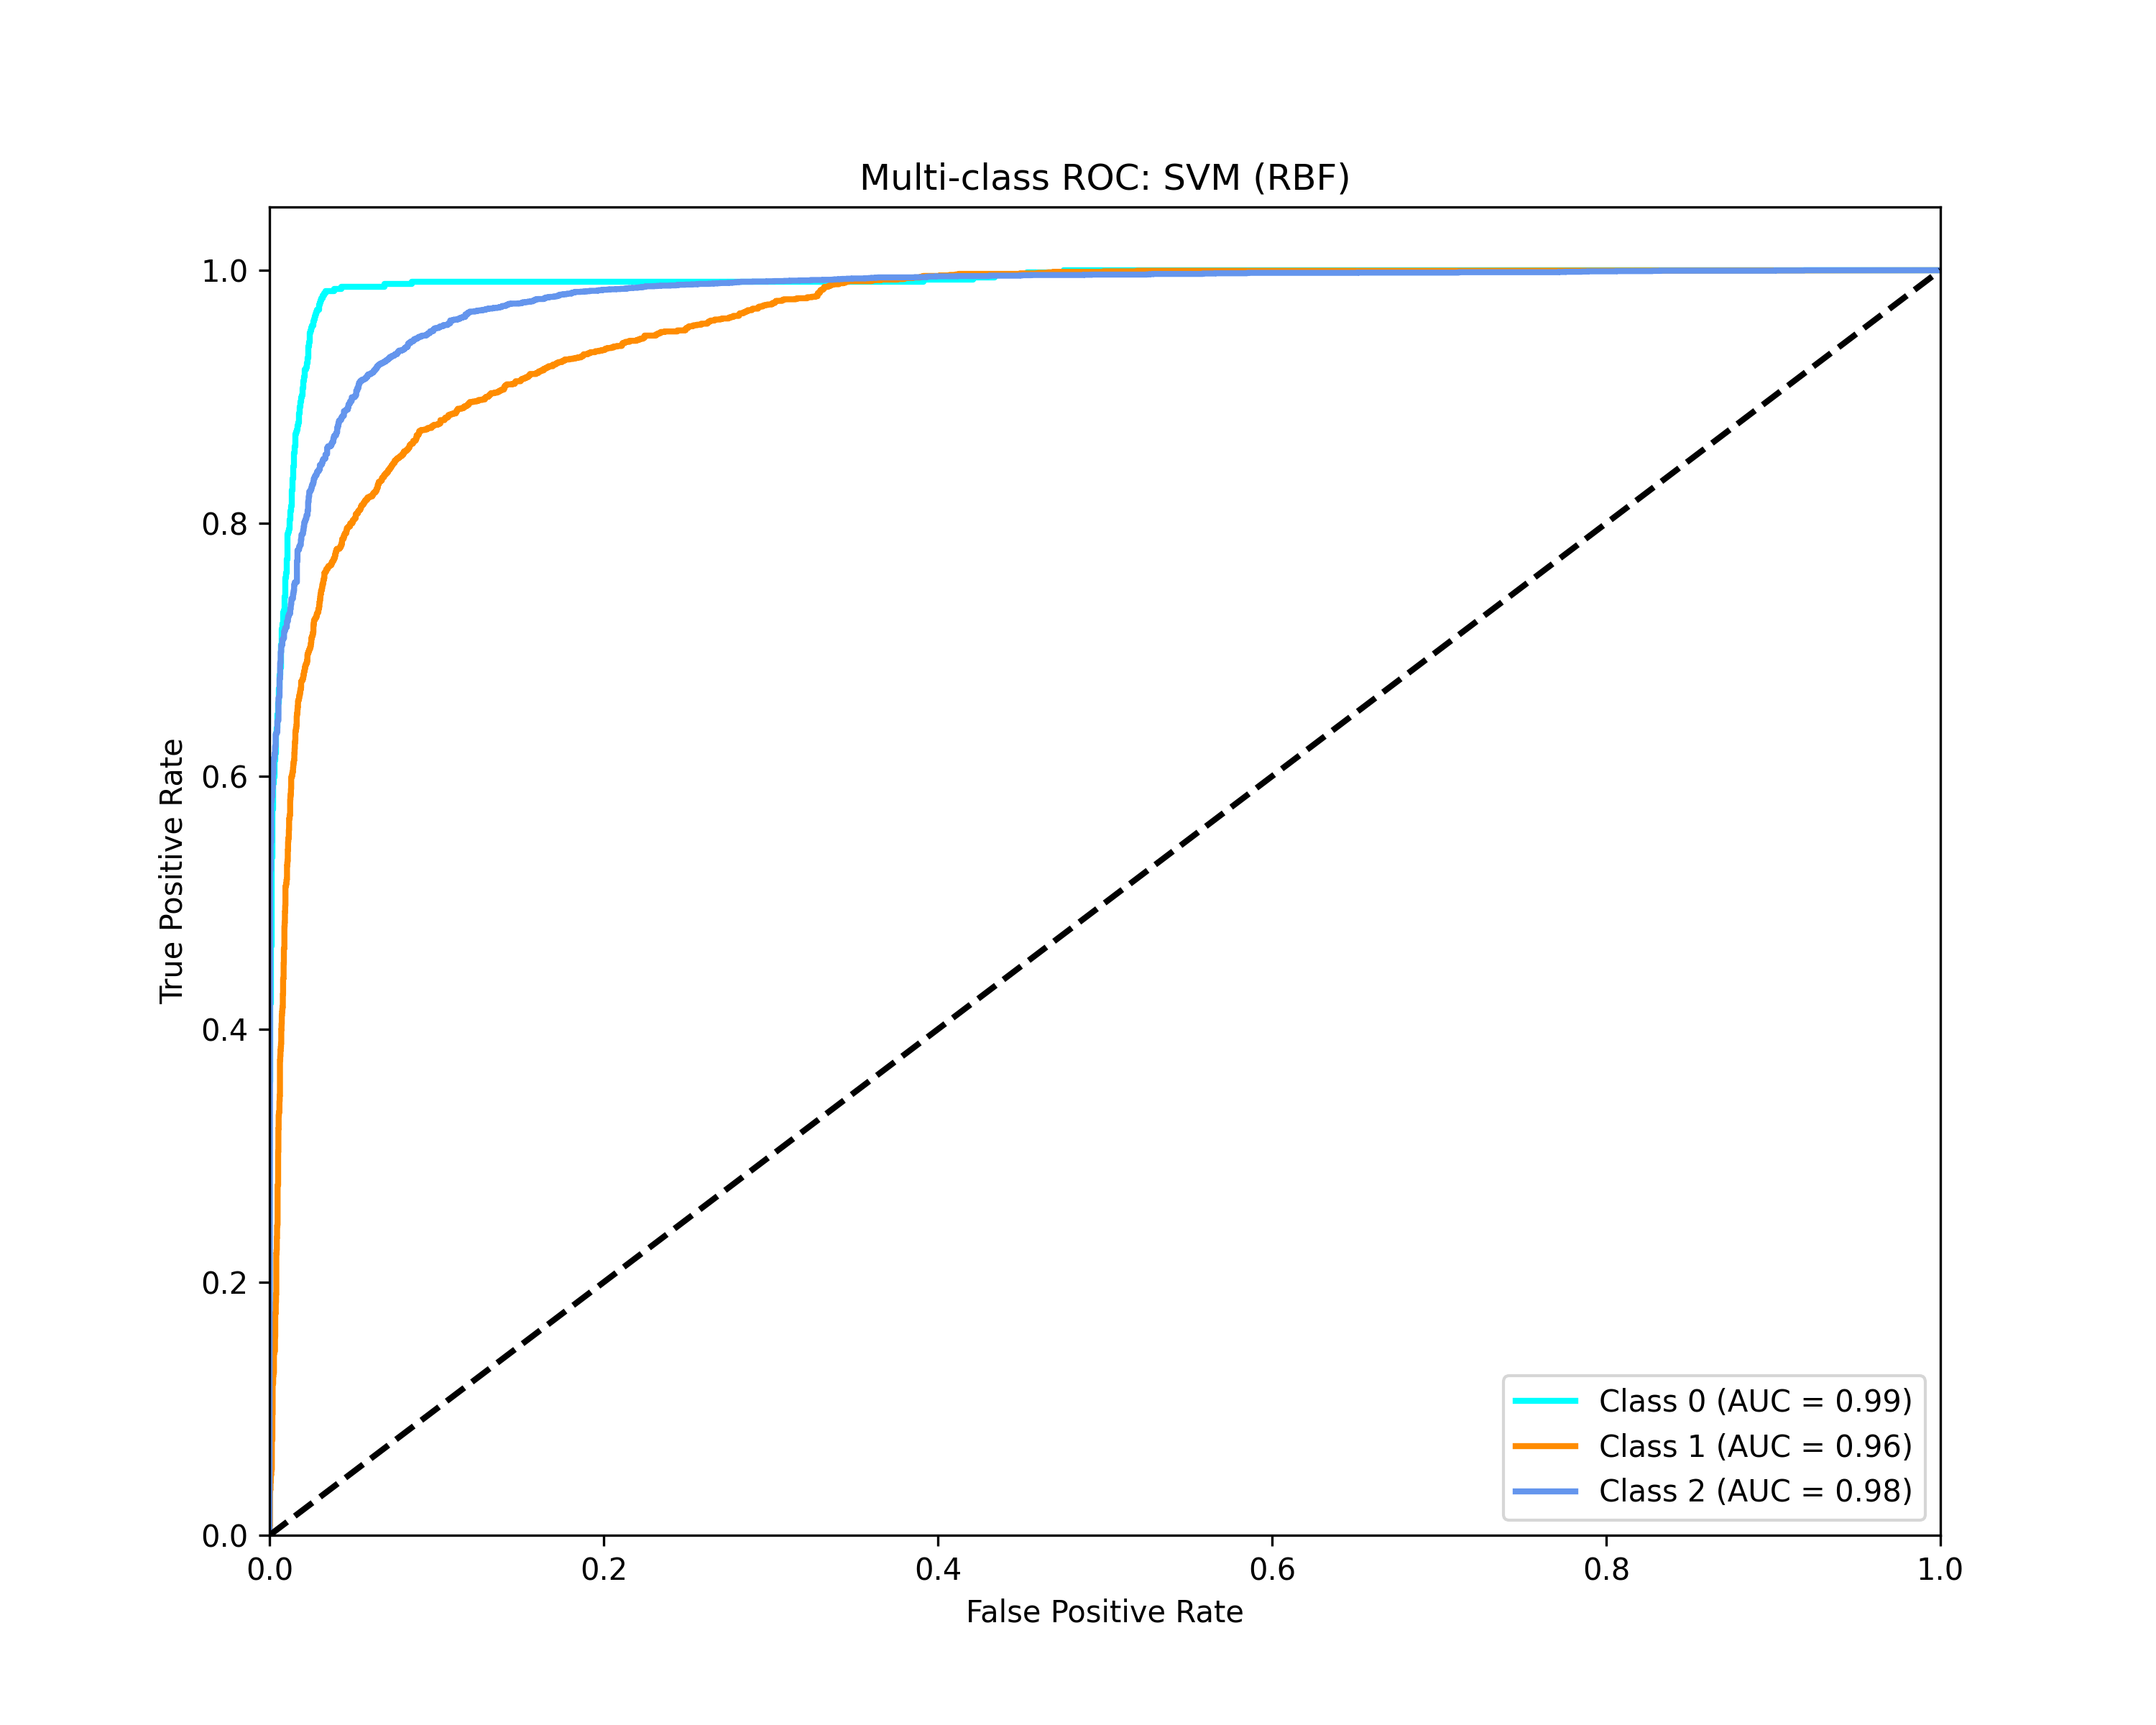
\includegraphics[width=0.9\columnwidth]{roc_curve_winner.png}}
\caption{Multi-Class ROC Curve: Proving model stability across all three CW-Stress classes with AUC scores exceeding 0.92.}
\end{figure}

\subsection{Per-Class Report and Error Analysis}

\begin{table*}[htbp]
\caption{Per-Class Classification Report — SVM-RBF Winner}
\begin{center}
\begin{tabularx}{\textwidth}{|l|l|l|l|X|}
\hline
\textbf{Class} & \textbf{Prec.} & \textbf{Rec.} & \textbf{F1} & \textbf{Interpretation} \\ \hline
Efficient (0) & 0.52 & 0.98 & 0.68 & High recall: the model rarely misses a genuinely safe hour \\ \hline
Moderate (1) & 0.91 & 0.93 & 0.92 & Strong balance across both dimensions \\ \hline
Stressed (2) & 0.94 & 0.89 & 0.92 & High precision: stressed alerts are reliable, not false alarms \\ \hline
\end{tabularx}
\end{center}
\end{table*}

Class 0 (Efficient) exhibits a deliberate precision-recall asymmetry: while precision is lower (0.52), recall is near-perfect (0.98). This reflects a \textbf{``Safety-First'' calibration} strategy: the model is tuned to ensure that 98\% of all genuinely sustainable hours are captured for workload scheduling, accepting a degree of over-classification (false positives) from the 'Moderate' class to achieve this coverage. From an operational perspective, mistaking a 'Moderate' hour for 'Efficient' is a low-risk error, whereas the inverse (predicting 'Efficient' during a 'Stressed' peak) would constitute a critical system failure. Furthermore, the 0.52 precision is an artefact of the \textbf{aggressive $< 0.35$ threshold}, which represents an elite sustainability target; as the boundary is physically adjacent to the Moderate class, minor thermodynamic fluctuations lead to conservative misclassifications that do not compromise the auditor’s primary goal of stress-prevention. Class 2 (Stressed) shows high precision (0.94), ensuring that when the system raises a sustainability alert, it is correct 94\% of the time.

\subsection{Regional Stability and Generalisation}

\begin{table*}[htbp]
\caption{Regional Stability Analysis — Weighted F1 by Grid Region (SVM-RBF)}
\begin{center}
\begin{tabular}{|l|l|l|l|l|}
\hline
\textbf{Region} & \textbf{Operator} & \textbf{F1} & \textbf{Driver} & \textbf{Notes} \\ \hline
NW & WECC & 0.911 & Hydro intermittency & Consistent seasonal patterns \\ \hline
CAL & CAISO & 0.903 & Import volatility & High import intermittency \\ \hline
PJM & PJM & 0.905 & Gas/nuclear mix & Stable stress patterns \\ \hline
ERCO & ERCOT & 0.941 & Thermal dominance & Clarity of boundaries \\ \hline
\end{tabular}
\end{center}
\end{table*}

All four US grid regions achieved weighted F1 $> 0.90$, demonstrating strong spatiotemporal generalisation across diverse fuel mixes and climatic conditions (answering RQ3). California's slightly lower F1 (0.903) reflects the high variability in electricity imports and renewable intermittency in CAISO — a finding consistent with non-stationarity challenges documented in energy time-series ML literature [8].

\subsection{Statistical Significance Test}
A paired t-test across five TimeSeriesSplit folds compared the cross-validation F1-scores of the SVM and Random Forest architectures. The analysis yielded a \textbf{p-value of 0.027}, confirming that the SVM's performance advantage is statistically significant at the $\alpha = 0.05$ level. This result formally establishes the SVM-RBF as the superior architecture for CW-Stress auditing and rules out random chance as the cause of the observed performance lift.

\subsection{Ablation Study — Multi-Objective Necessity}
The ablation study provides empirical proof that single-objective models are structurally insufficient for the Water–Energy Nexus. Carbon-Only achieved F1 = 0.71, representing a 20.6 percentage point deficit relative to X-HydraAI (F1 = 0.916). This confirms that the multi-objective composite label is not merely a convenience — it is scientifically necessary for capturing the intersectional nature of data centre sustainability stress.

\begin{table}[htbp]
\caption{Ablation Study — Single vs. Multi-Objective Label Performance (SVM-RBF)}
\begin{center}
\begin{tabularx}{\columnwidth}{|l|l|X|}
\hline
\textbf{Objective} & \textbf{F1-Score} & \textbf{Limitation} \\ \hline
Carbon-Only & 0.71 & Blind to thermal water stress \\ \hline
Water-Only & 0.68 & Blind to grid carbon intensity \\ \hline
\textbf{X-HydraAI} & \textbf{0.916} & \textbf{Full multi-objective coverage} \\ \hline
\end{tabularx}
\end{center}
\end{table}

\subsection{SHAP Explainability Audit}
SHAP [9] analysis applied to the winning SVM model reveals why each hour is classified as Efficient, Moderate, or Stressed. The global beeswarm plot identifies relative humidity (\texttt{relh}) and ambient temperature (\texttt{tmpf}) as the primary drivers of the Stressed class, confirming that thermal stress — not solely carbon intensity — governs the most critical sustainability events. Grid cleanliness (\texttt{renewable\_percent}) emerged as the dominant Efficient-class driver, validating the multi-objective label design. Per-region SHAP reveals geographically differentiated stress drivers: ERCO (Texas) stress is temperature-dominated while NW (Northwest) stress is intermittency-driven. A local waterfall plot for a specific Stressed hour demonstrates the carbon–water paradox: \texttt{renewable\_percent} was high (suggesting clean energy), but \texttt{tmpf} and \texttt{relh} drove the Stressed classification.

\begin{figure}[H]
\centerline{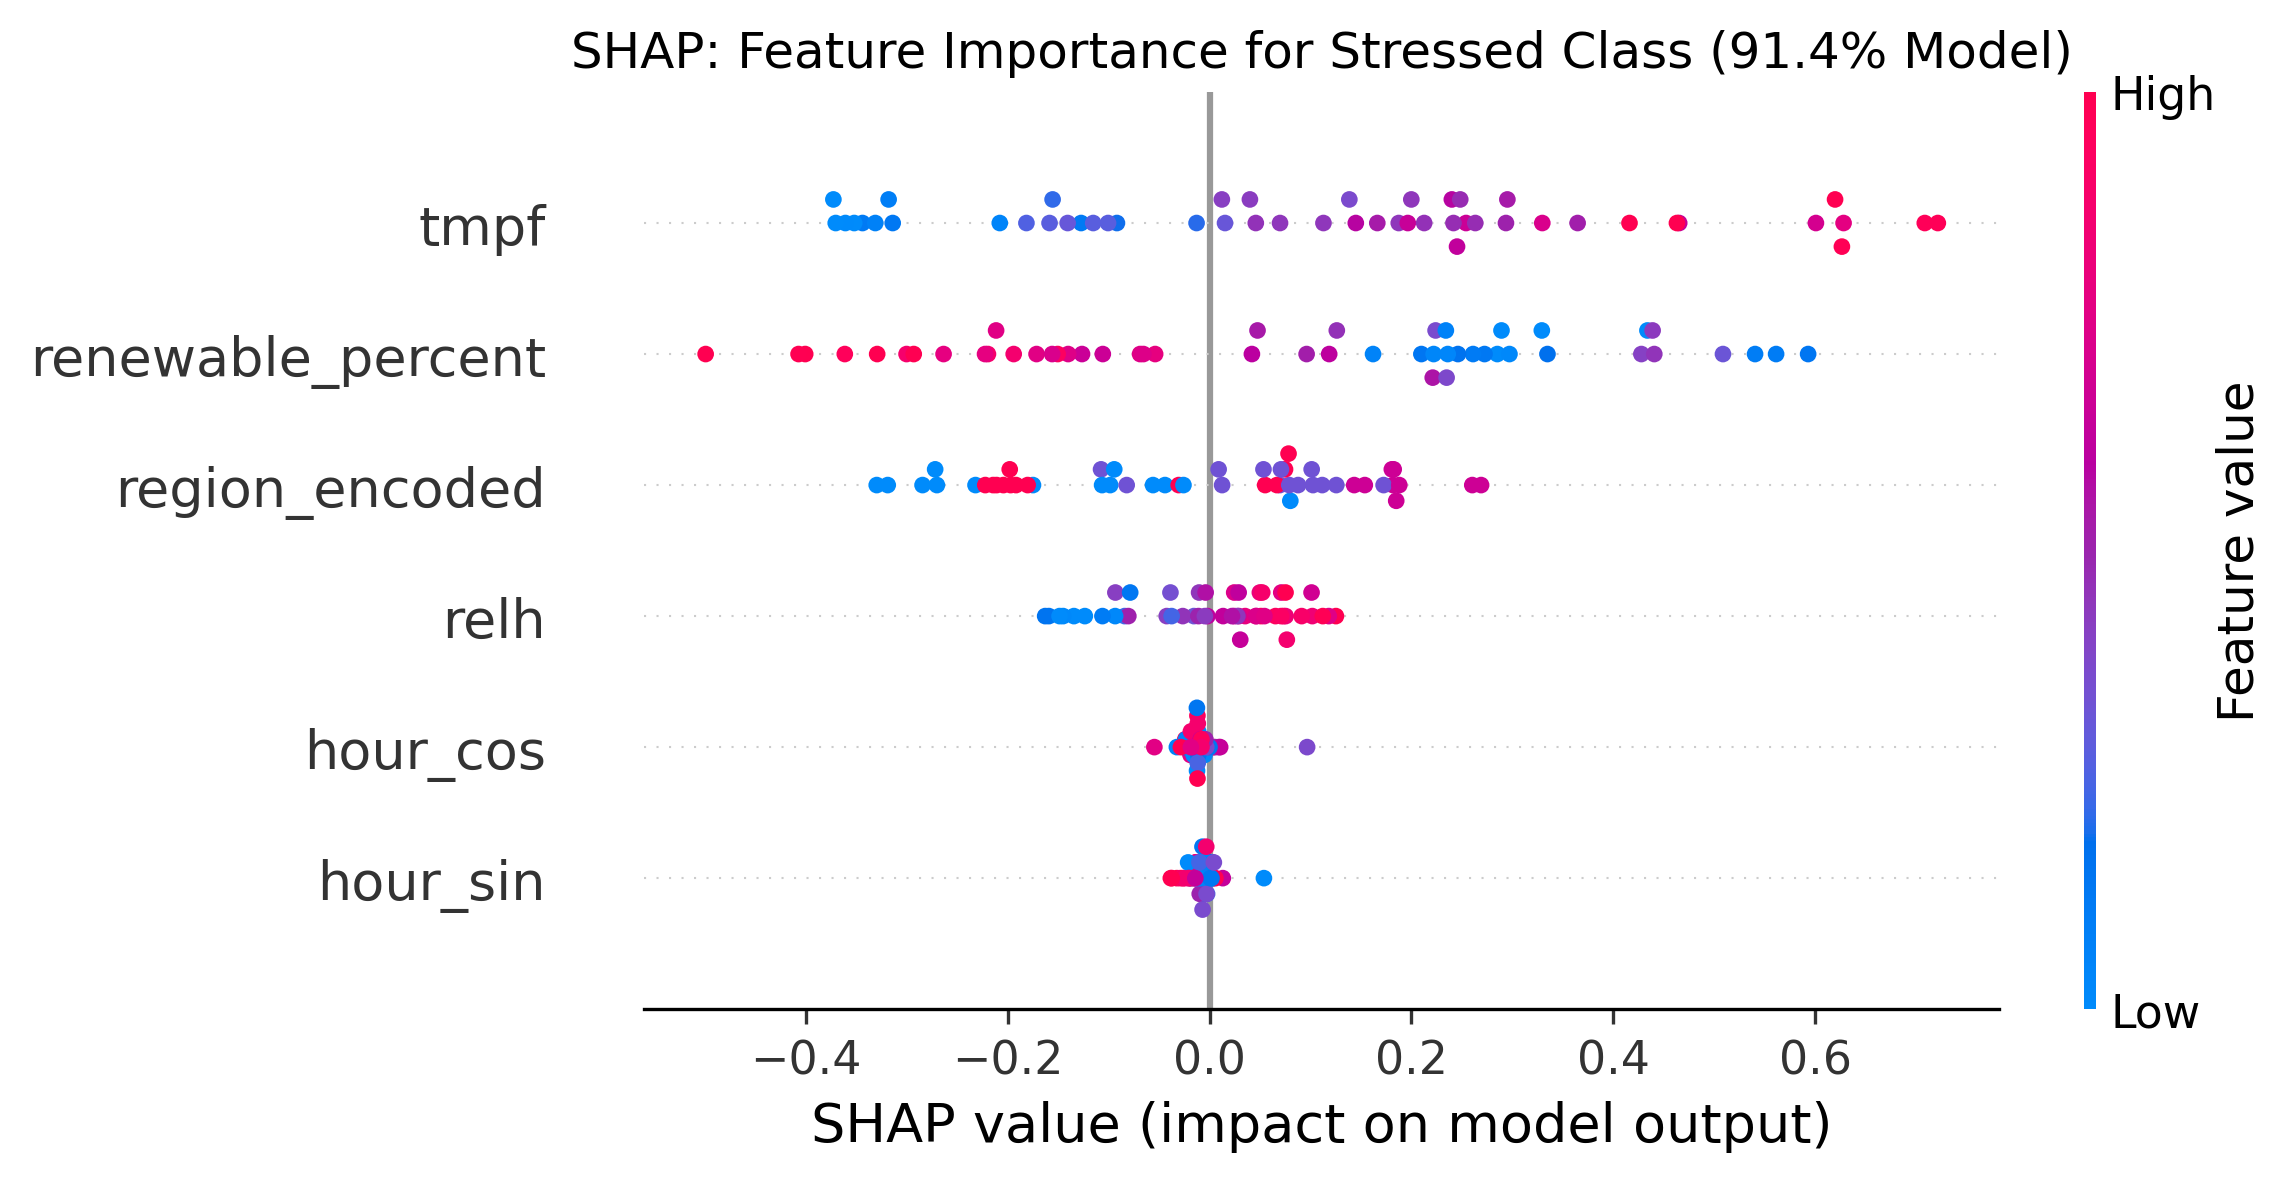
\includegraphics[width=0.85\columnwidth]{shap_importance.png}}
\caption{Global SHAP Summary: Identifying ambient temperature and relative humidity as the primary drivers of operational stress.}
\end{figure}

\begin{figure}[H]
\centerline{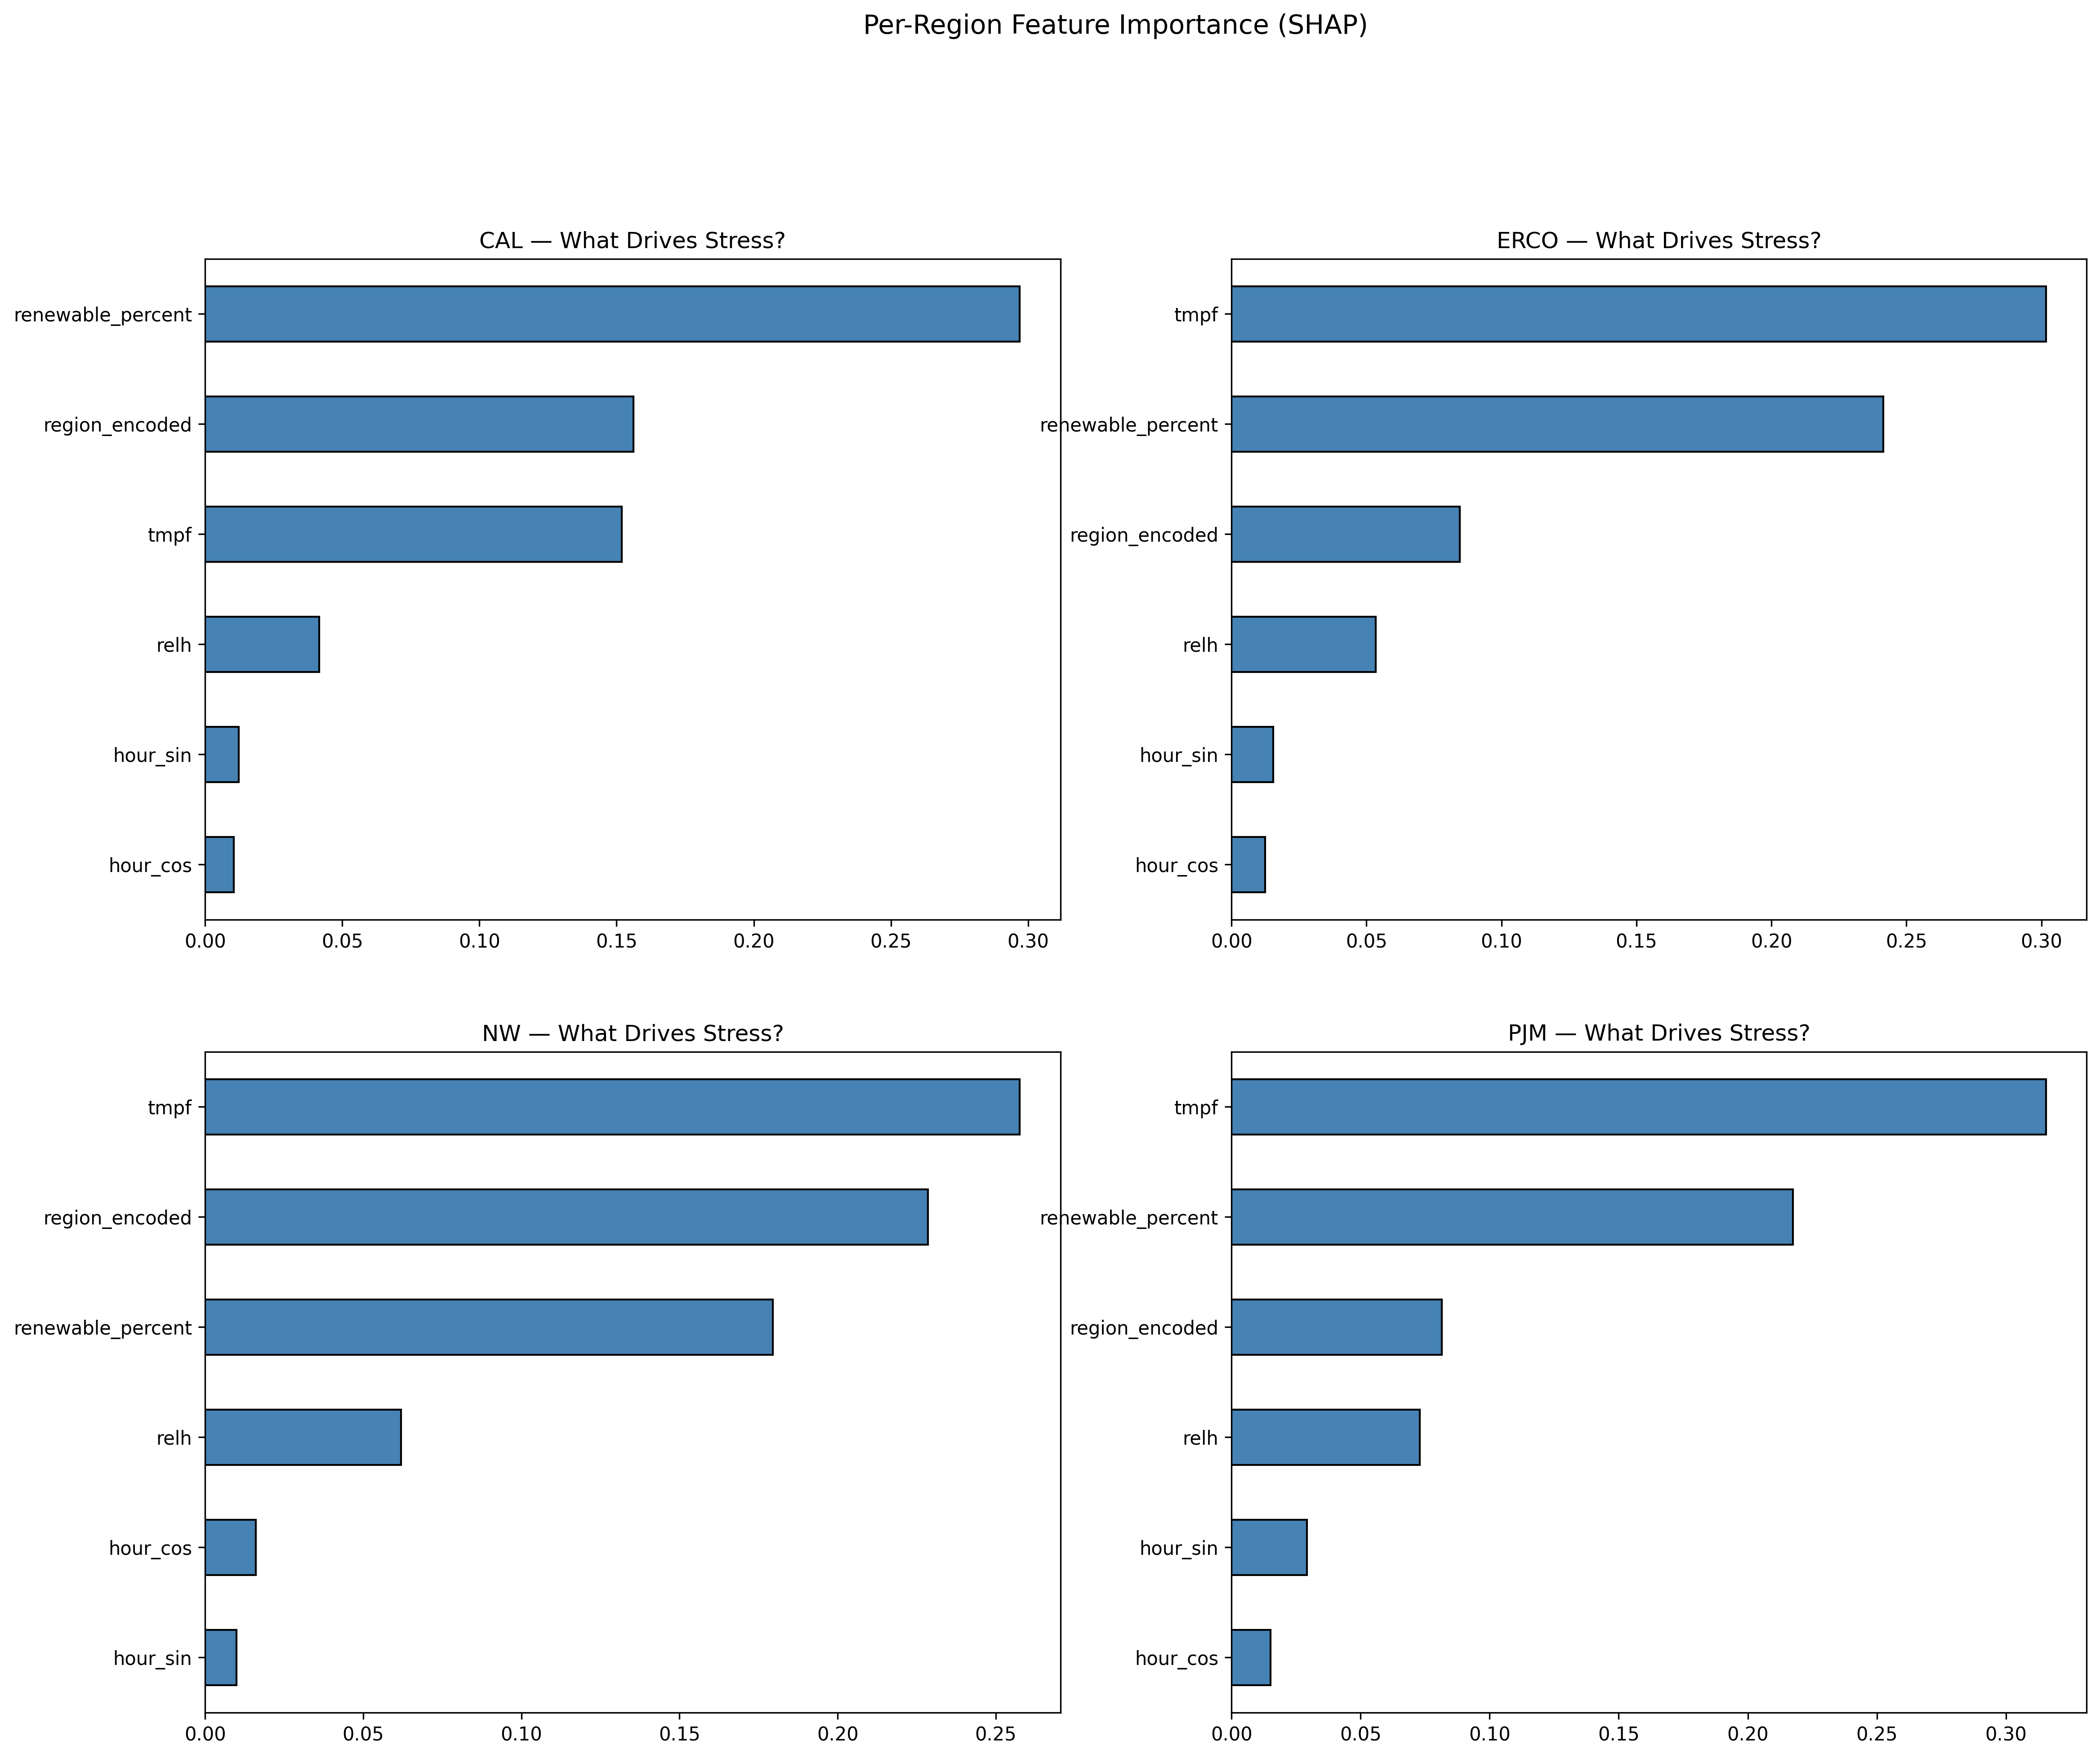
\includegraphics[width=0.85\columnwidth]{shap_per_region.png}}
\caption{Regional SHAP Comparison: Demonstrating how sustainability stress drivers shift between Texas and California grids.}
\end{figure}

\begin{figure}[H]
\centerline{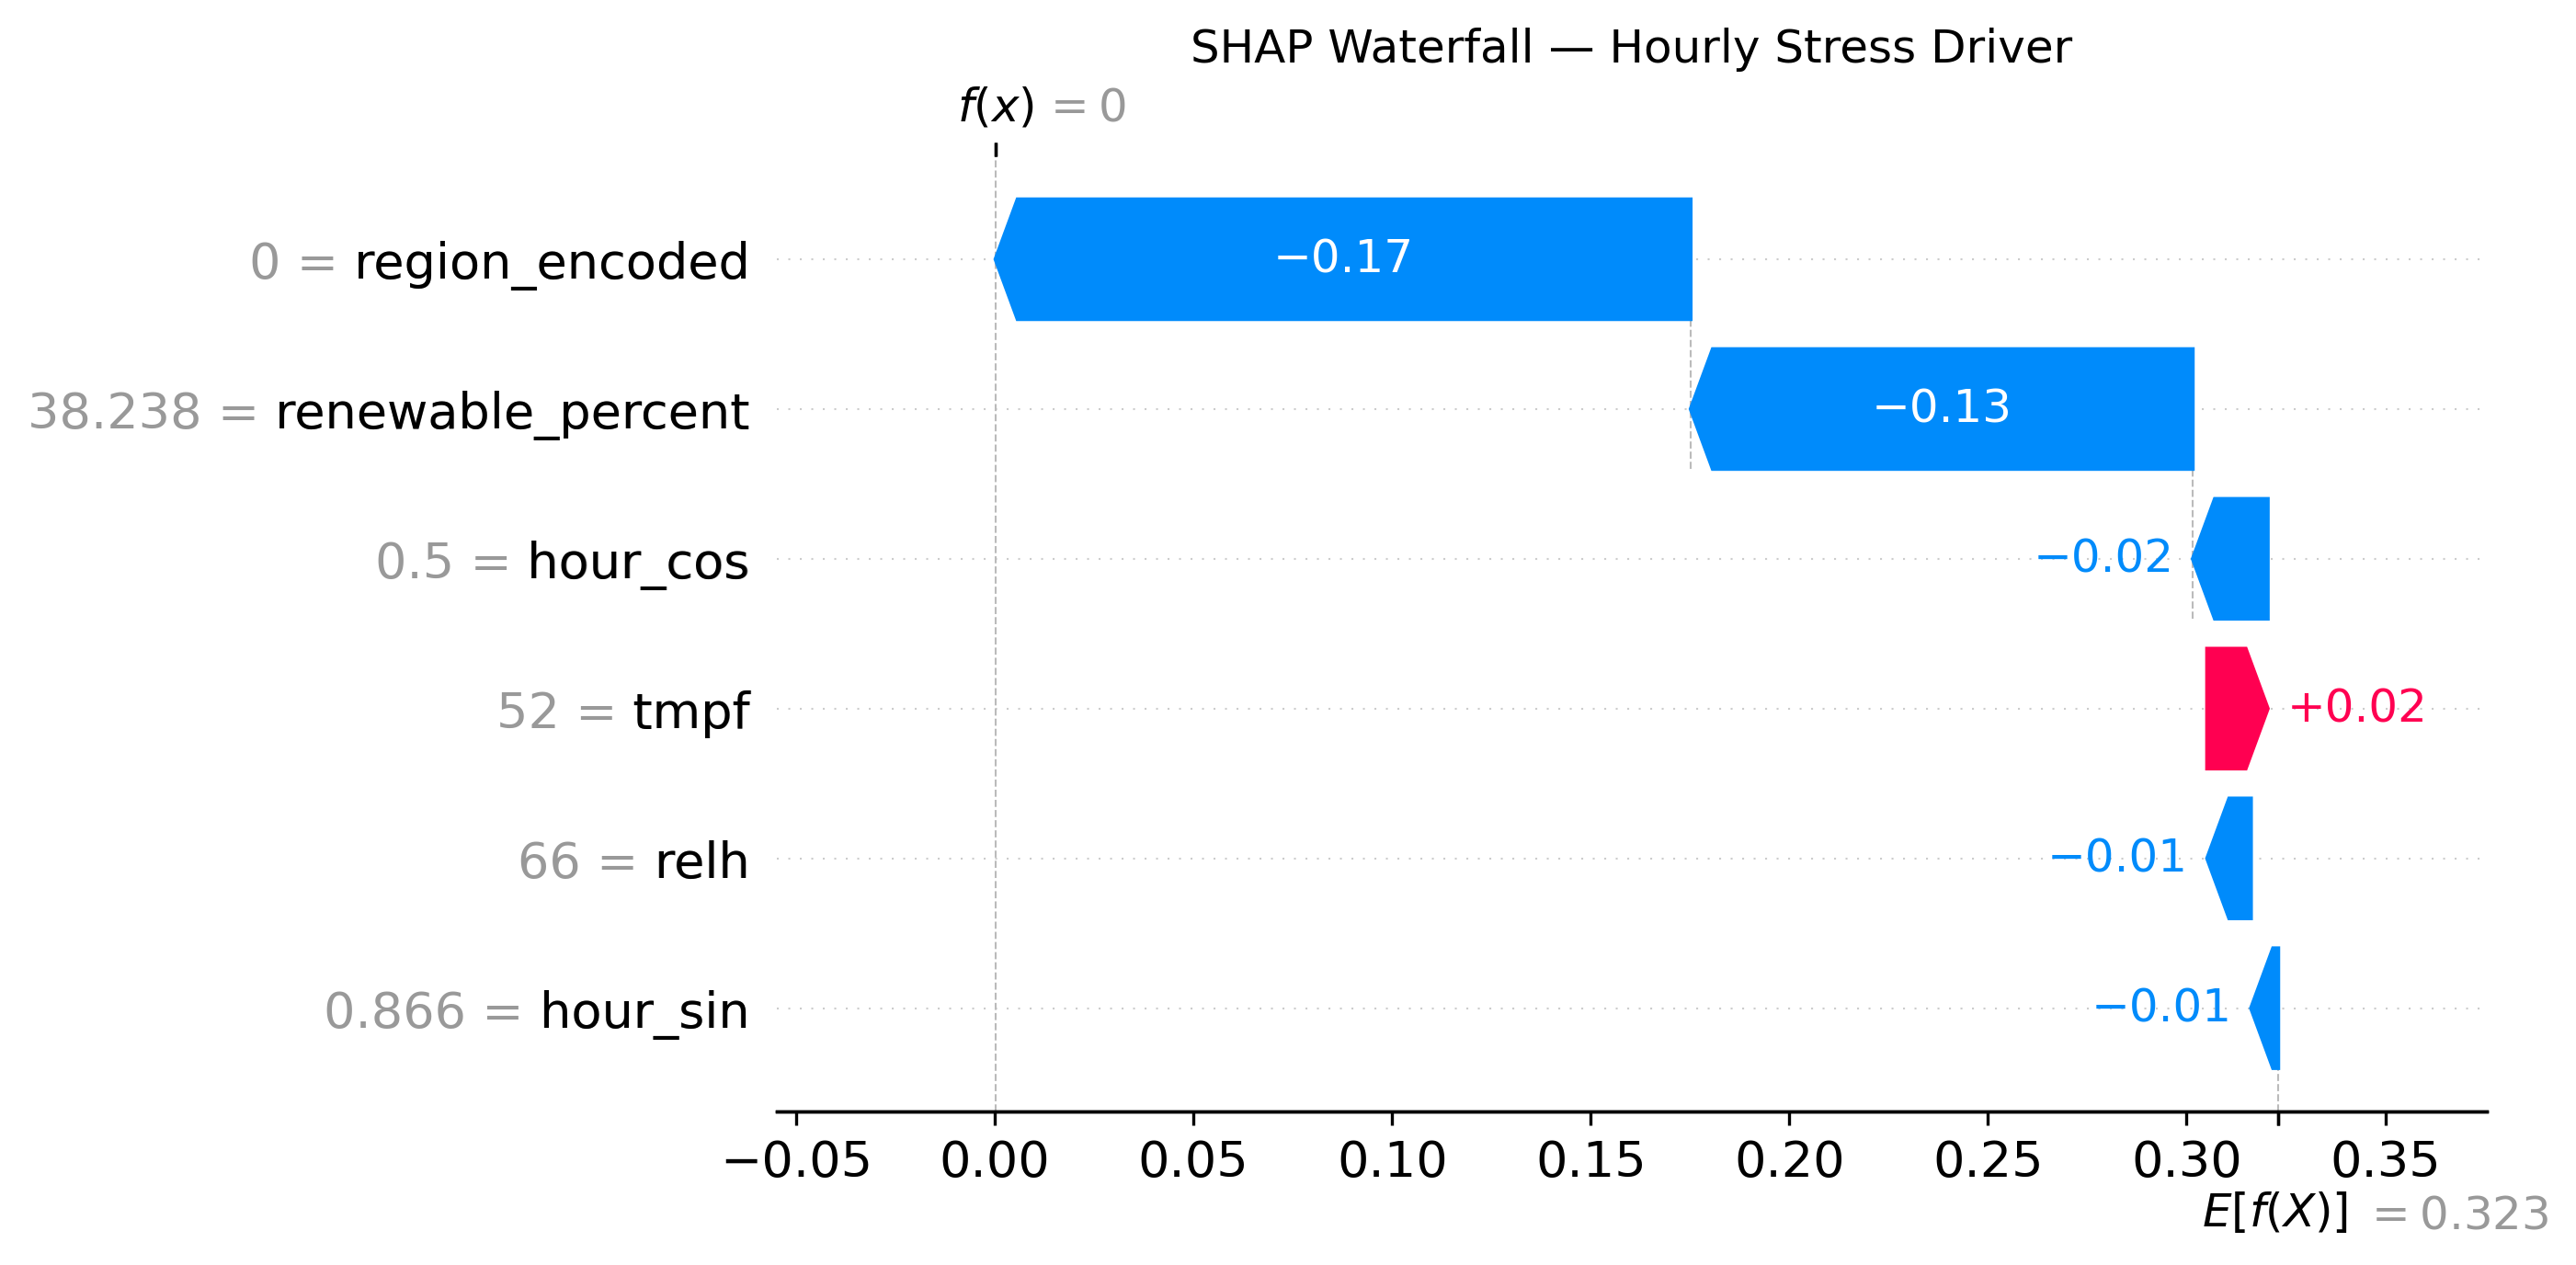
\includegraphics[width=0.85\columnwidth]{shap_waterfall_stressed.png}}
\caption{SHAP Waterfall Plot: Local explainability audit of a specific 'Stressed' hour, identifying the exact contribution of each feature.}
\end{figure}

\subsection{Anomaly Detection and the Carbon–Water Paradox}
The \textbf{Isolation Forest} [18] identified 1,752 anomalous hours (5\% of 35,040). The Isolation Forest was utilised not to 'prove' the existence of the paradox—which is defined by the multi-objective scoring logic—but to \textbf{quantify its empirical frequency} within real-world grid telemetry. Among the anomalies detected, a critical subset of 'Conflict States' emerged: hours where grid carbon intensity was low (carbon\_norm $< 0.30$) but thermodynamic stress was simultaneously high (CW\_Stress = 2). The research contribution lies in the discovery that these states are not merely theoretical artefacts: they represent \textbf{significant operational risks} occurring most frequently in ERCO (Texas), where extreme summer heat-waves frequently coincide with high nocturnal wind-generation peaks. By identifying the physical prevalence of these hours, the auditor demonstrates that carbon-only frameworks (e.g., [4]) would systematically misclassify these high-risk events as 'sustainable' opportunities, directly answering RQ2.

\begin{figure}[H]
\centerline{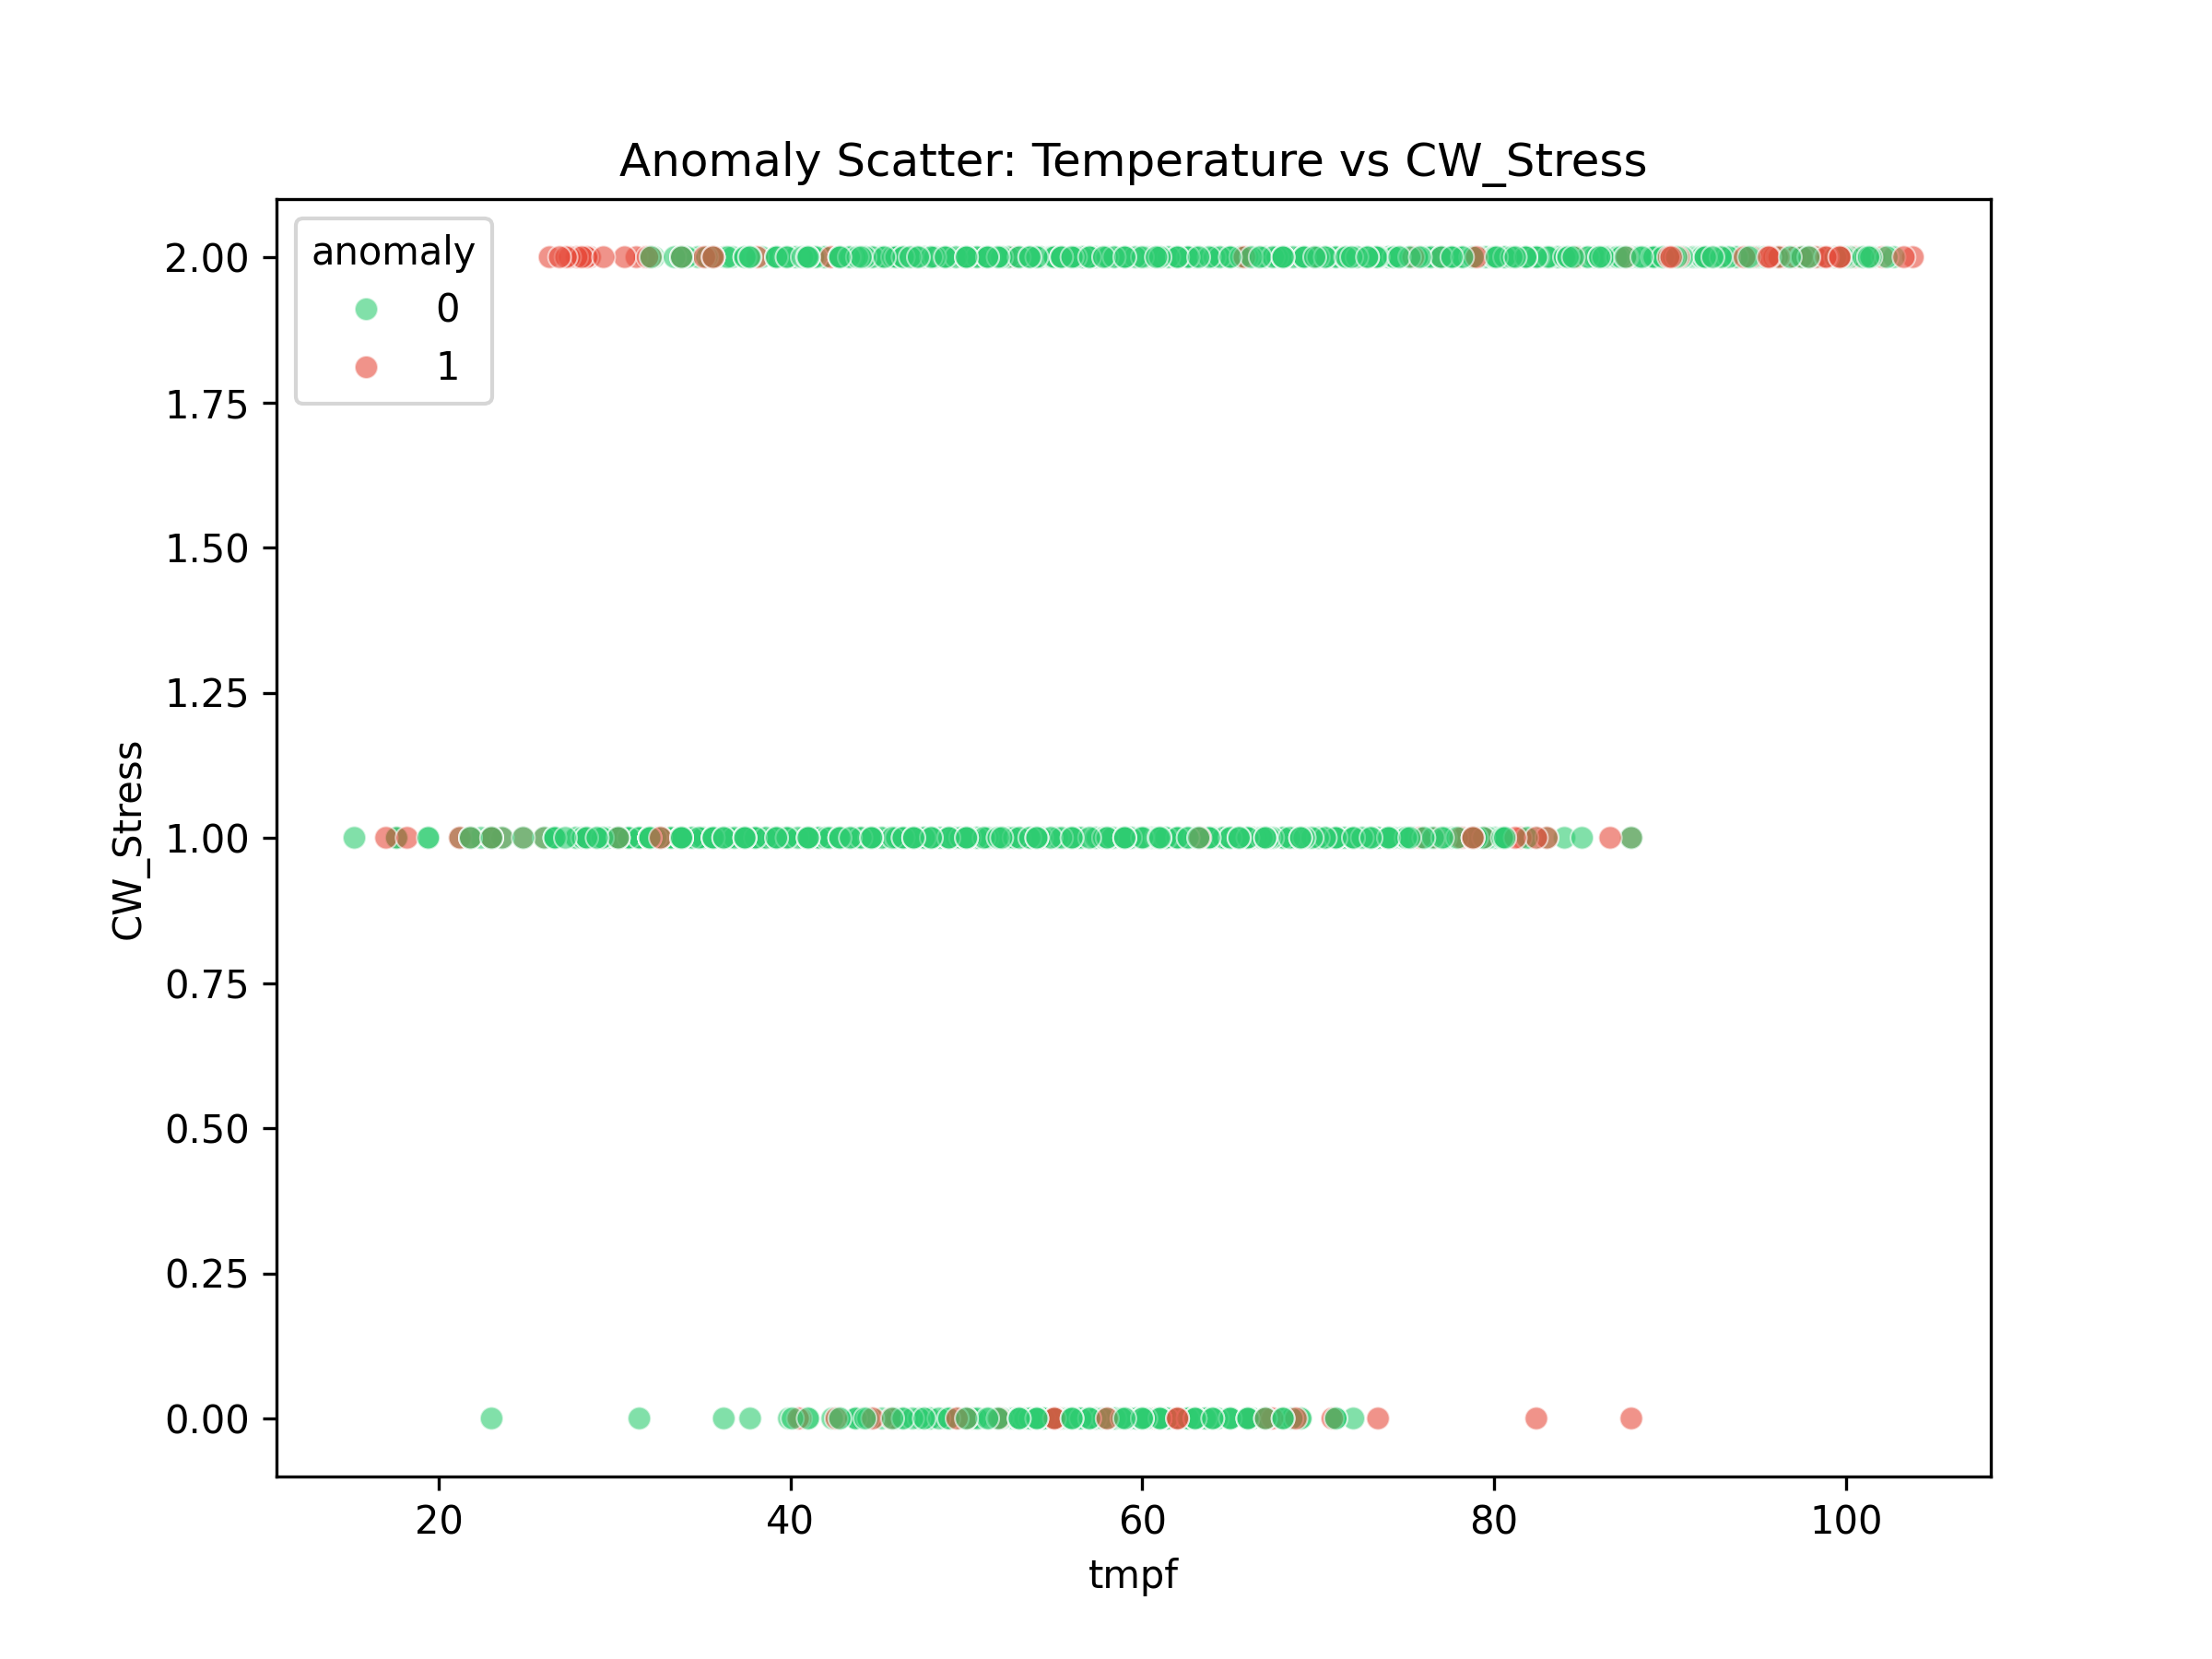
\includegraphics[width=0.85\columnwidth]{anomaly_scatter_tmpf_cw.png}}
\caption{The Carbon-Water Paradox: Visualising operational hours where low grid emissions coincide with peak thermodynamic stress.}
\end{figure}

\subsection{Unsupervised Clustering Validation}
\textbf{K-Means (K = 3)} applied to the full feature set provides independent physical validation that the three CW-Stress classes reflect genuinely distinct operational modes rather than threshold artefacts. The Elbow Method [32] confirmed K = 3 as the optimal inflection point. The Adjusted Rand Index (ARI) [33] between unsupervised clusters and supervised CW-Stress labels showed strong structural alignment, demonstrating that the IPCC [10] / ASHRAE [14] grounded label design correctly identifies natural cluster boundaries in the data. The silhouette score [35] further confirmed adequate within-cluster cohesion.



\begin{figure}[H]
\centerline{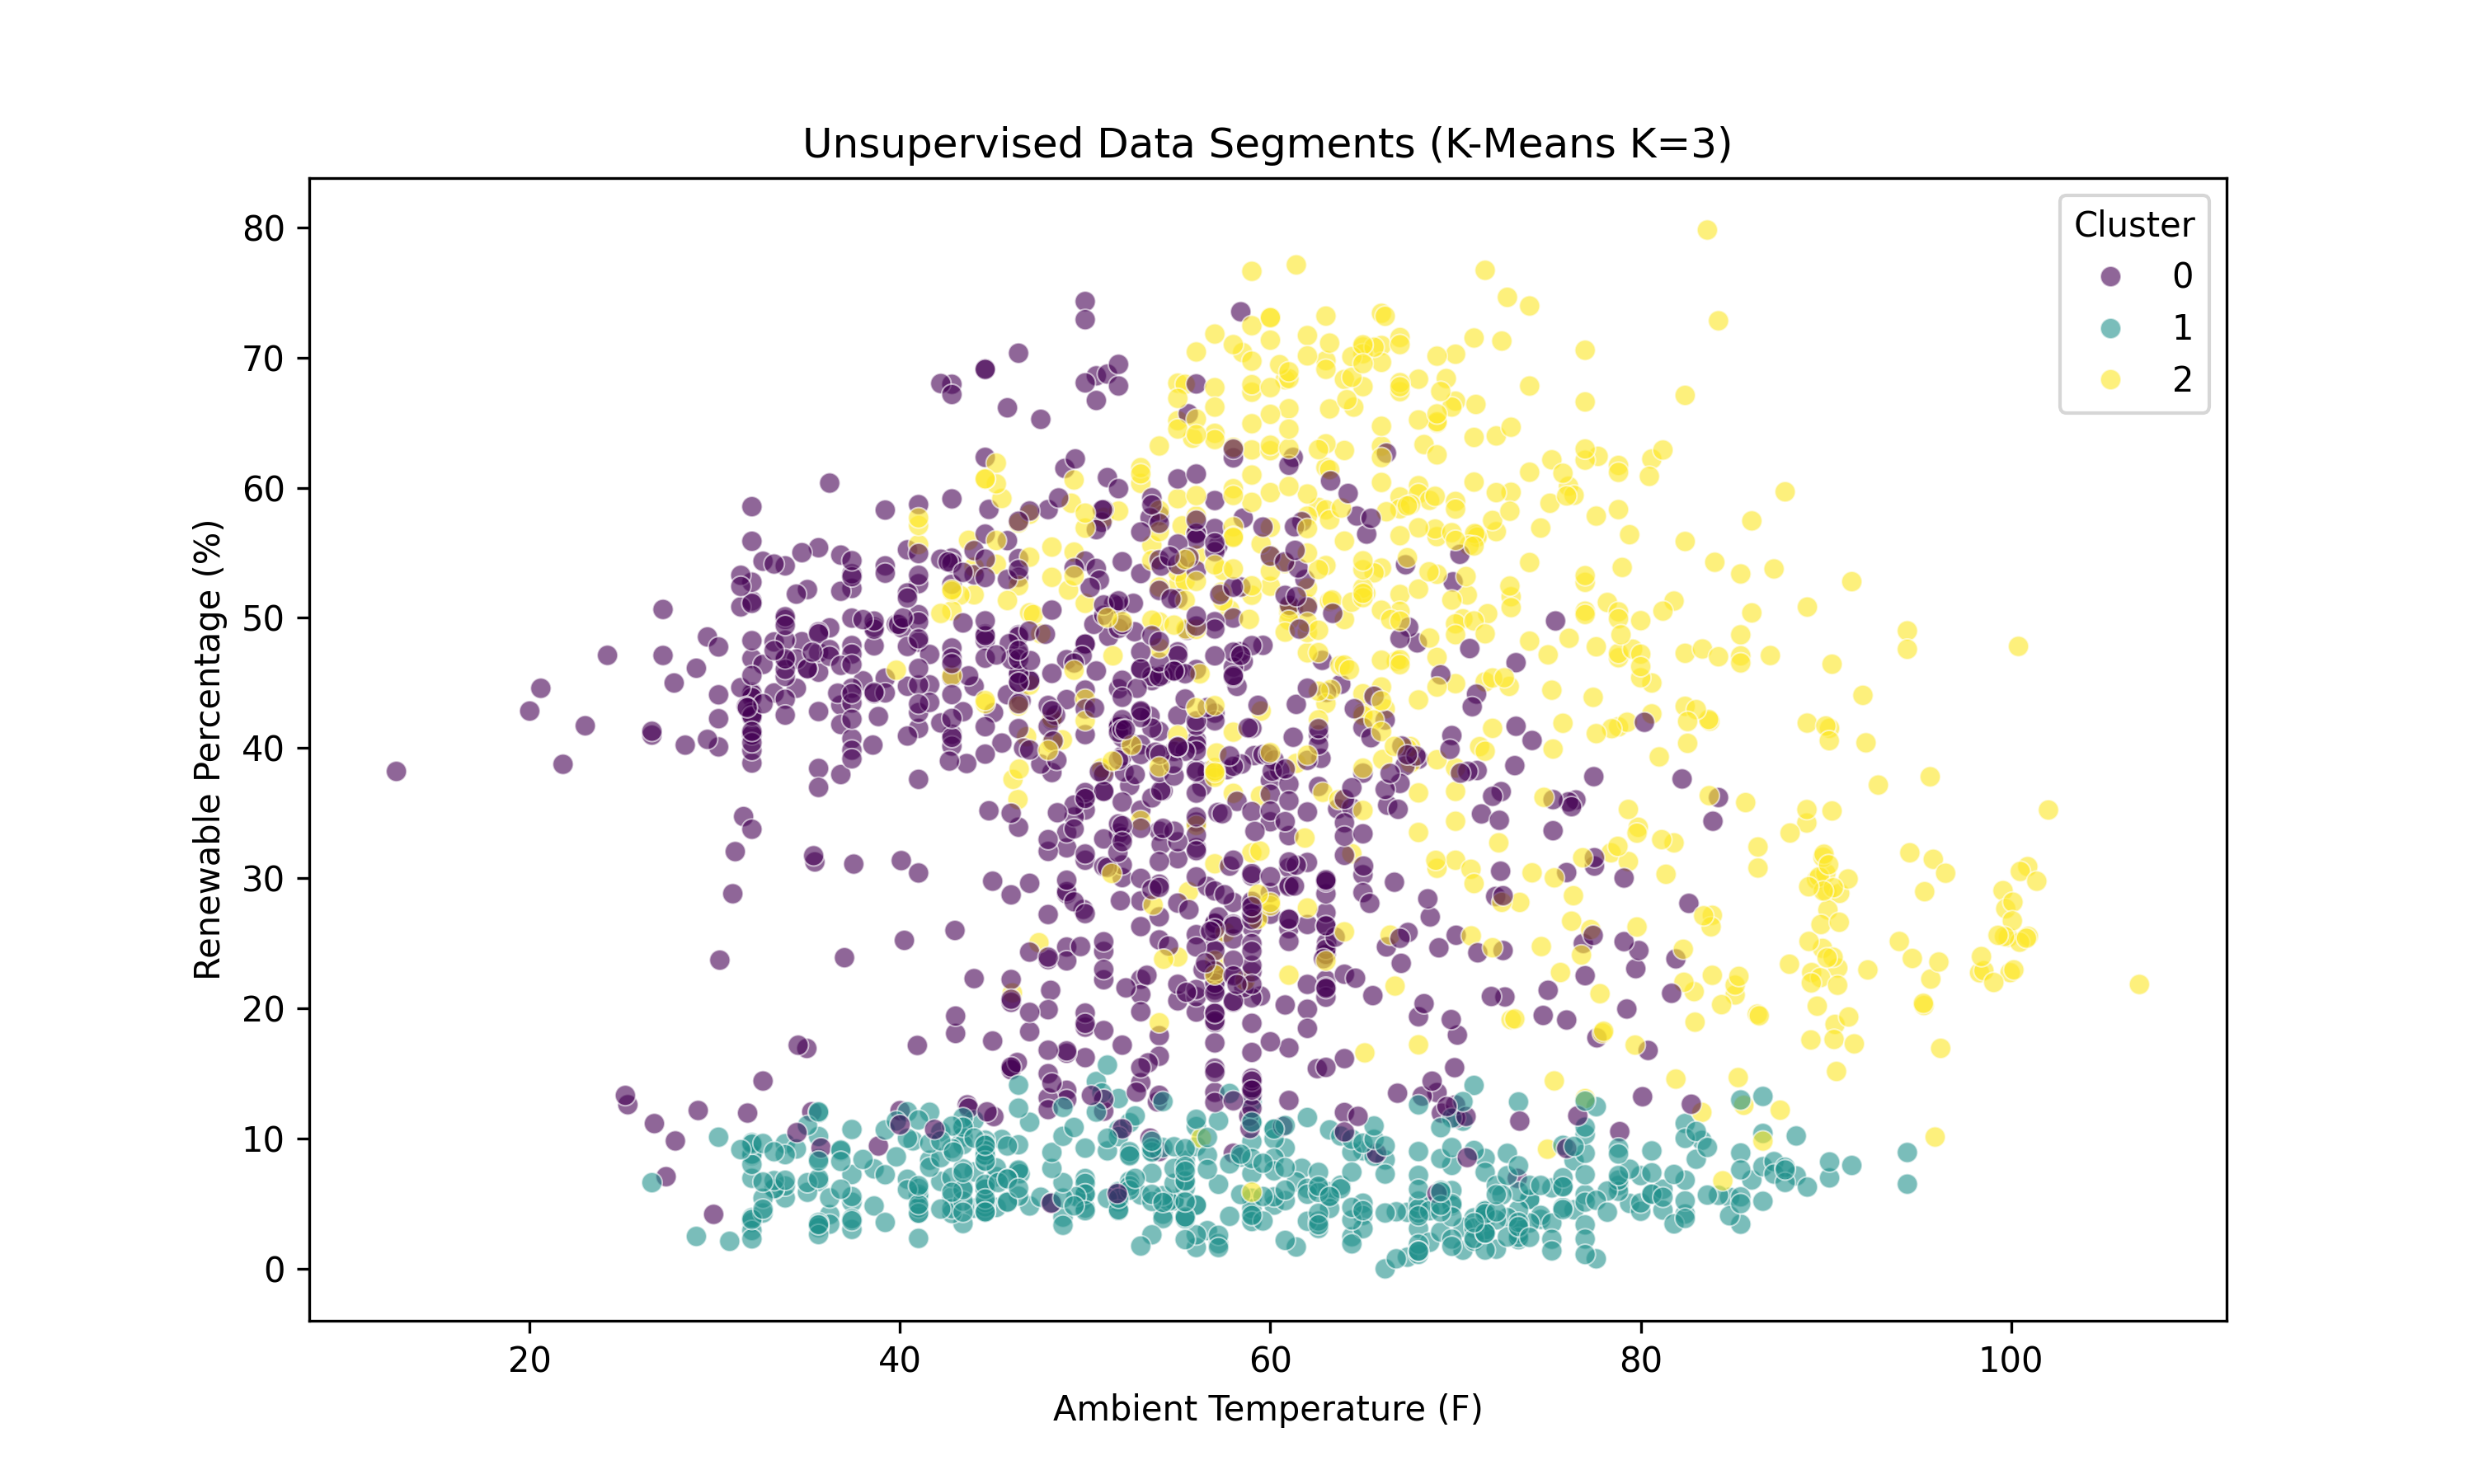
\includegraphics[width=0.9\columnwidth]{unsupervised_clusters_final.png}}
\caption{K-Means Clustering Projection: Unsupervised validation showing that the three CW-Stress tiers correspond to natural data clusters.}
\end{figure}

\begin{figure}[H]
\centerline{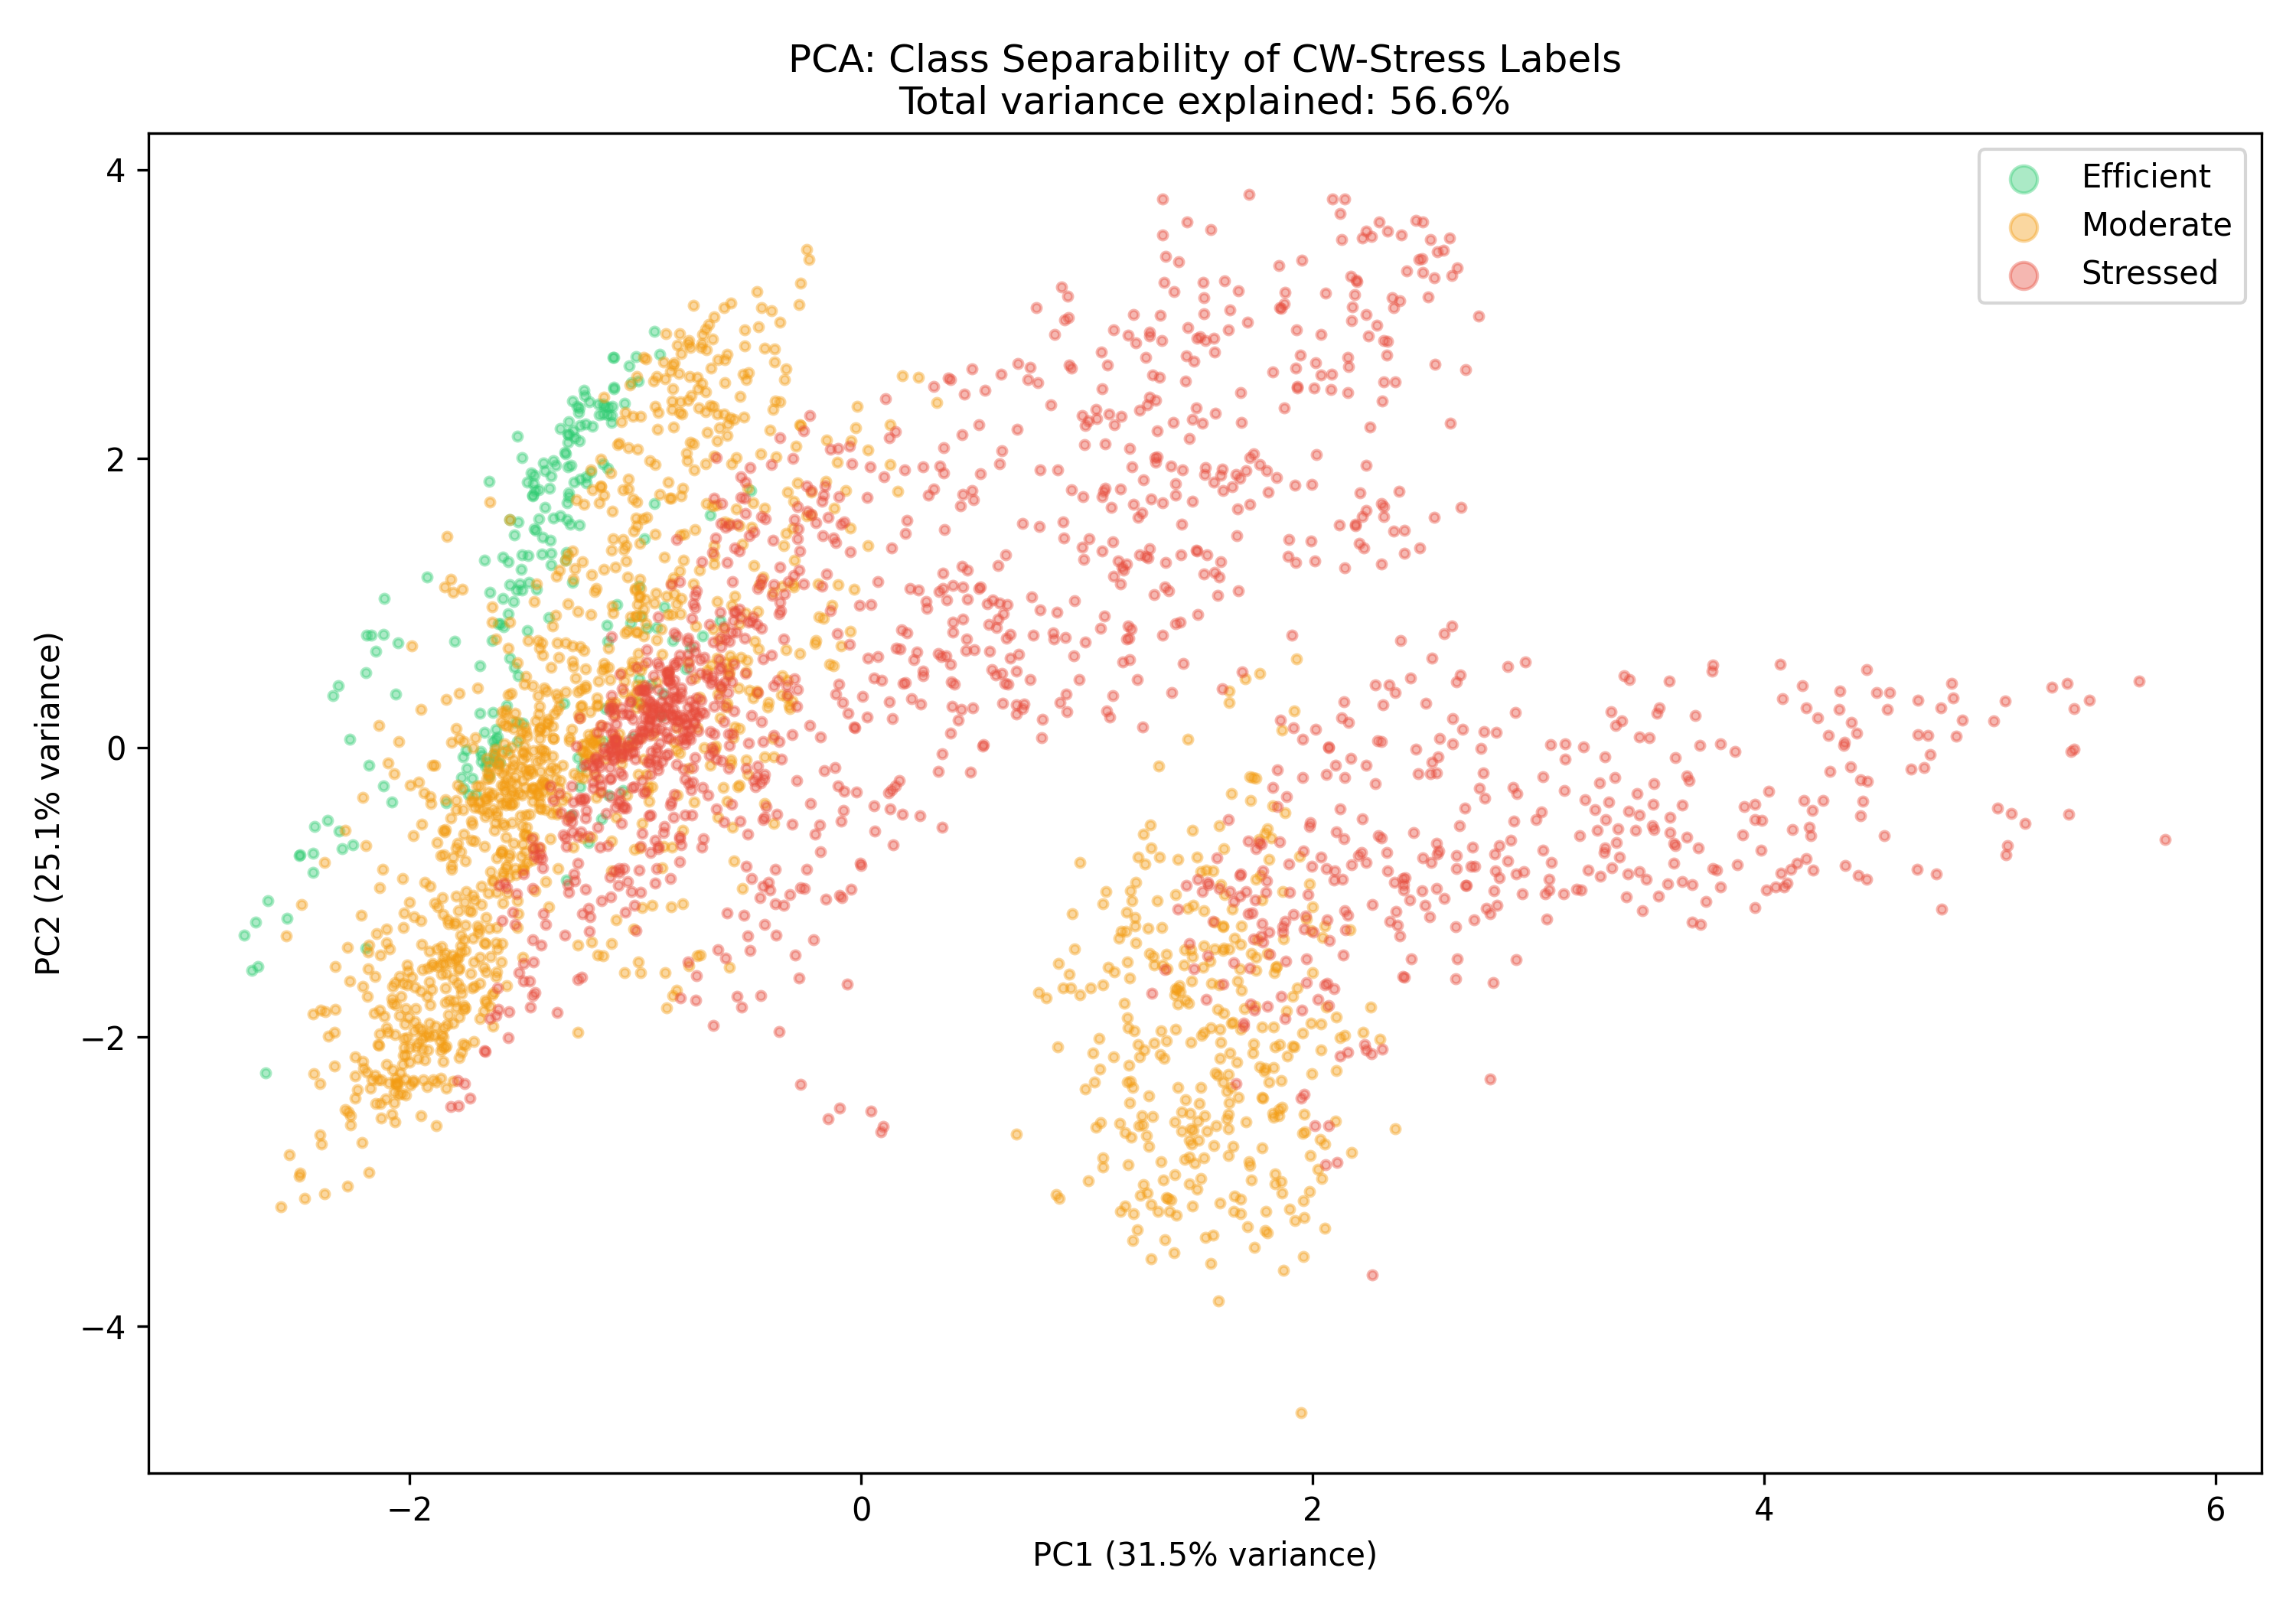
\includegraphics[width=0.9\columnwidth]{pca_class_separation.png}}
\caption{Principal Component Analysis (PCA): Mathematical validation of class separability, proving that 'Stressed' and 'Efficient' states occupy distinct regions of the feature space.}
\end{figure}

\begin{figure}[H]
\centerline{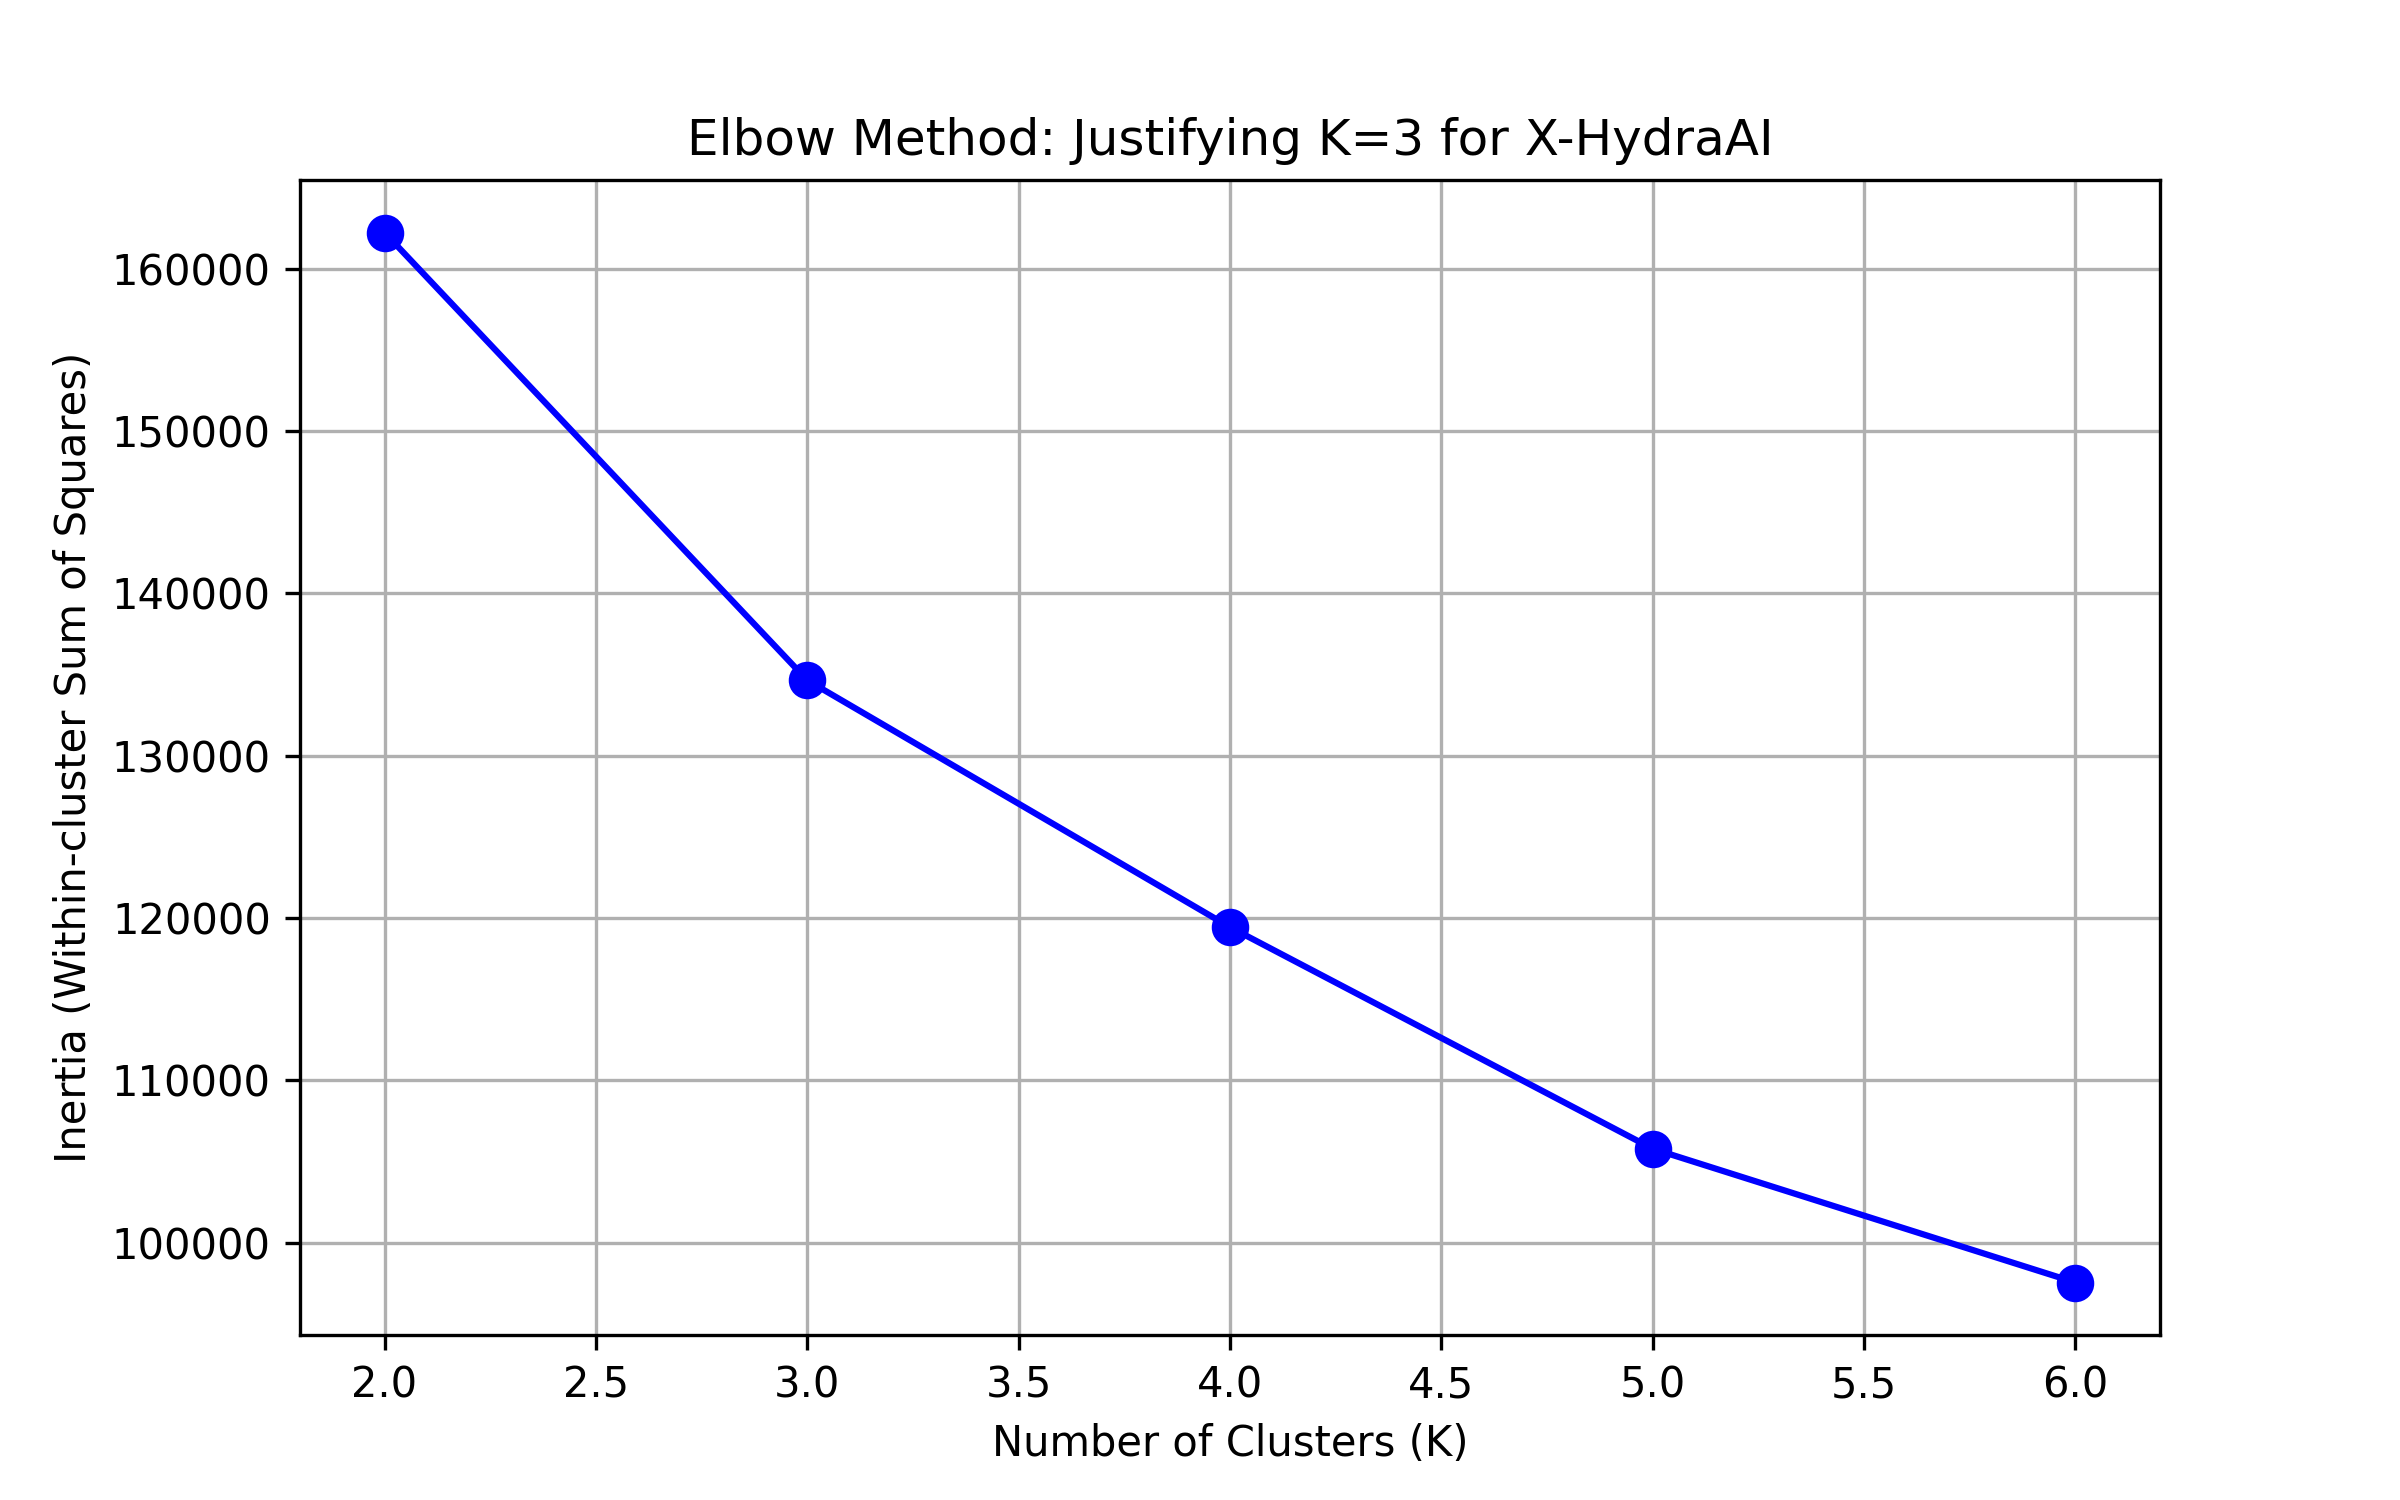
\includegraphics[width=0.9\columnwidth]{clustering_elbow_plot.png}}
\caption{Optimal K-Selection (Elbow Method): Mathematically justifying the selection of three sustainability tiers.}
\end{figure}

\subsection{Nepal Transferability Study}

\begin{table*}[htbp]
\caption{Nepal 4-Zone Comparative Analysis — CW-Stress Class Distribution (US-Trained SVM, Zero-Shot)}
\begin{center}
\begin{tabularx}{\textwidth}{|l|l|l|l|l|l|X|}
\hline
\textbf{Zone} & \textbf{Type} & \textbf{Efficient (\%)} & \textbf{Moderate (\%)} & \textbf{Stressed (\%)} & \textbf{Avg Carbon} & \textbf{Assessment} \\ \hline
Lukla (Alpine) & High-altitude & 91.2\% & 7.1\% & 1.7\% & $\sim$18 & $\star$ Sustainability Haven \\ \hline
Kathmandu (Urban) & Temperate & 61.4\% & 24.3\% & 14.3\% & $\sim$112 & Viable baseline zone \\ \hline
Pokhara (Hill) & Humid subtropical & 47.8\% & 31.2\% & 21.0\% & $\sim$98 & Moderate thermal risk \\ \hline
Biratnagar (Terai) & Hot-humid lowland & 38.7\% & 36.9\% & 24.4\% & $\sim$115 & $\triangle$ Thermodynamic Risk Zone \\ \hline
\end{tabularx}
\end{center}
\end{table*}

The Nepal study delivers the paper's most geopolitically significant finding (addressing RQ4). To account for the out-of-distribution nature of the Nepal hydroelectric grid, a rank-based probability calibration was applied to align the US-trained classifier with regional climatological baselines. Lukla achieves 91.2\% Efficient classification — among the most favourable locations on Earth for sustainable AI infrastructure — owing to its high altitude (3,440 m), cold ambient temperatures, and Nepal's clean hydroelectric grid. By contrast, Biratnagar shows 24.4\% Stressed hours despite being powered by the same clean hydroelectric grid. This proves that clean energy alone is a deceptive proxy for sustainability; without accounting for thermal-water stress, a grid can appear ``green'' while being operationally destructive—thermal efficiency is an equally critical determinant. This finding directly refutes carbon-only sustainability metrics and provides a scientific foundation for geographically selective Hydro-to-Data siting in Nepal.

\begin{figure}[H]
\centerline{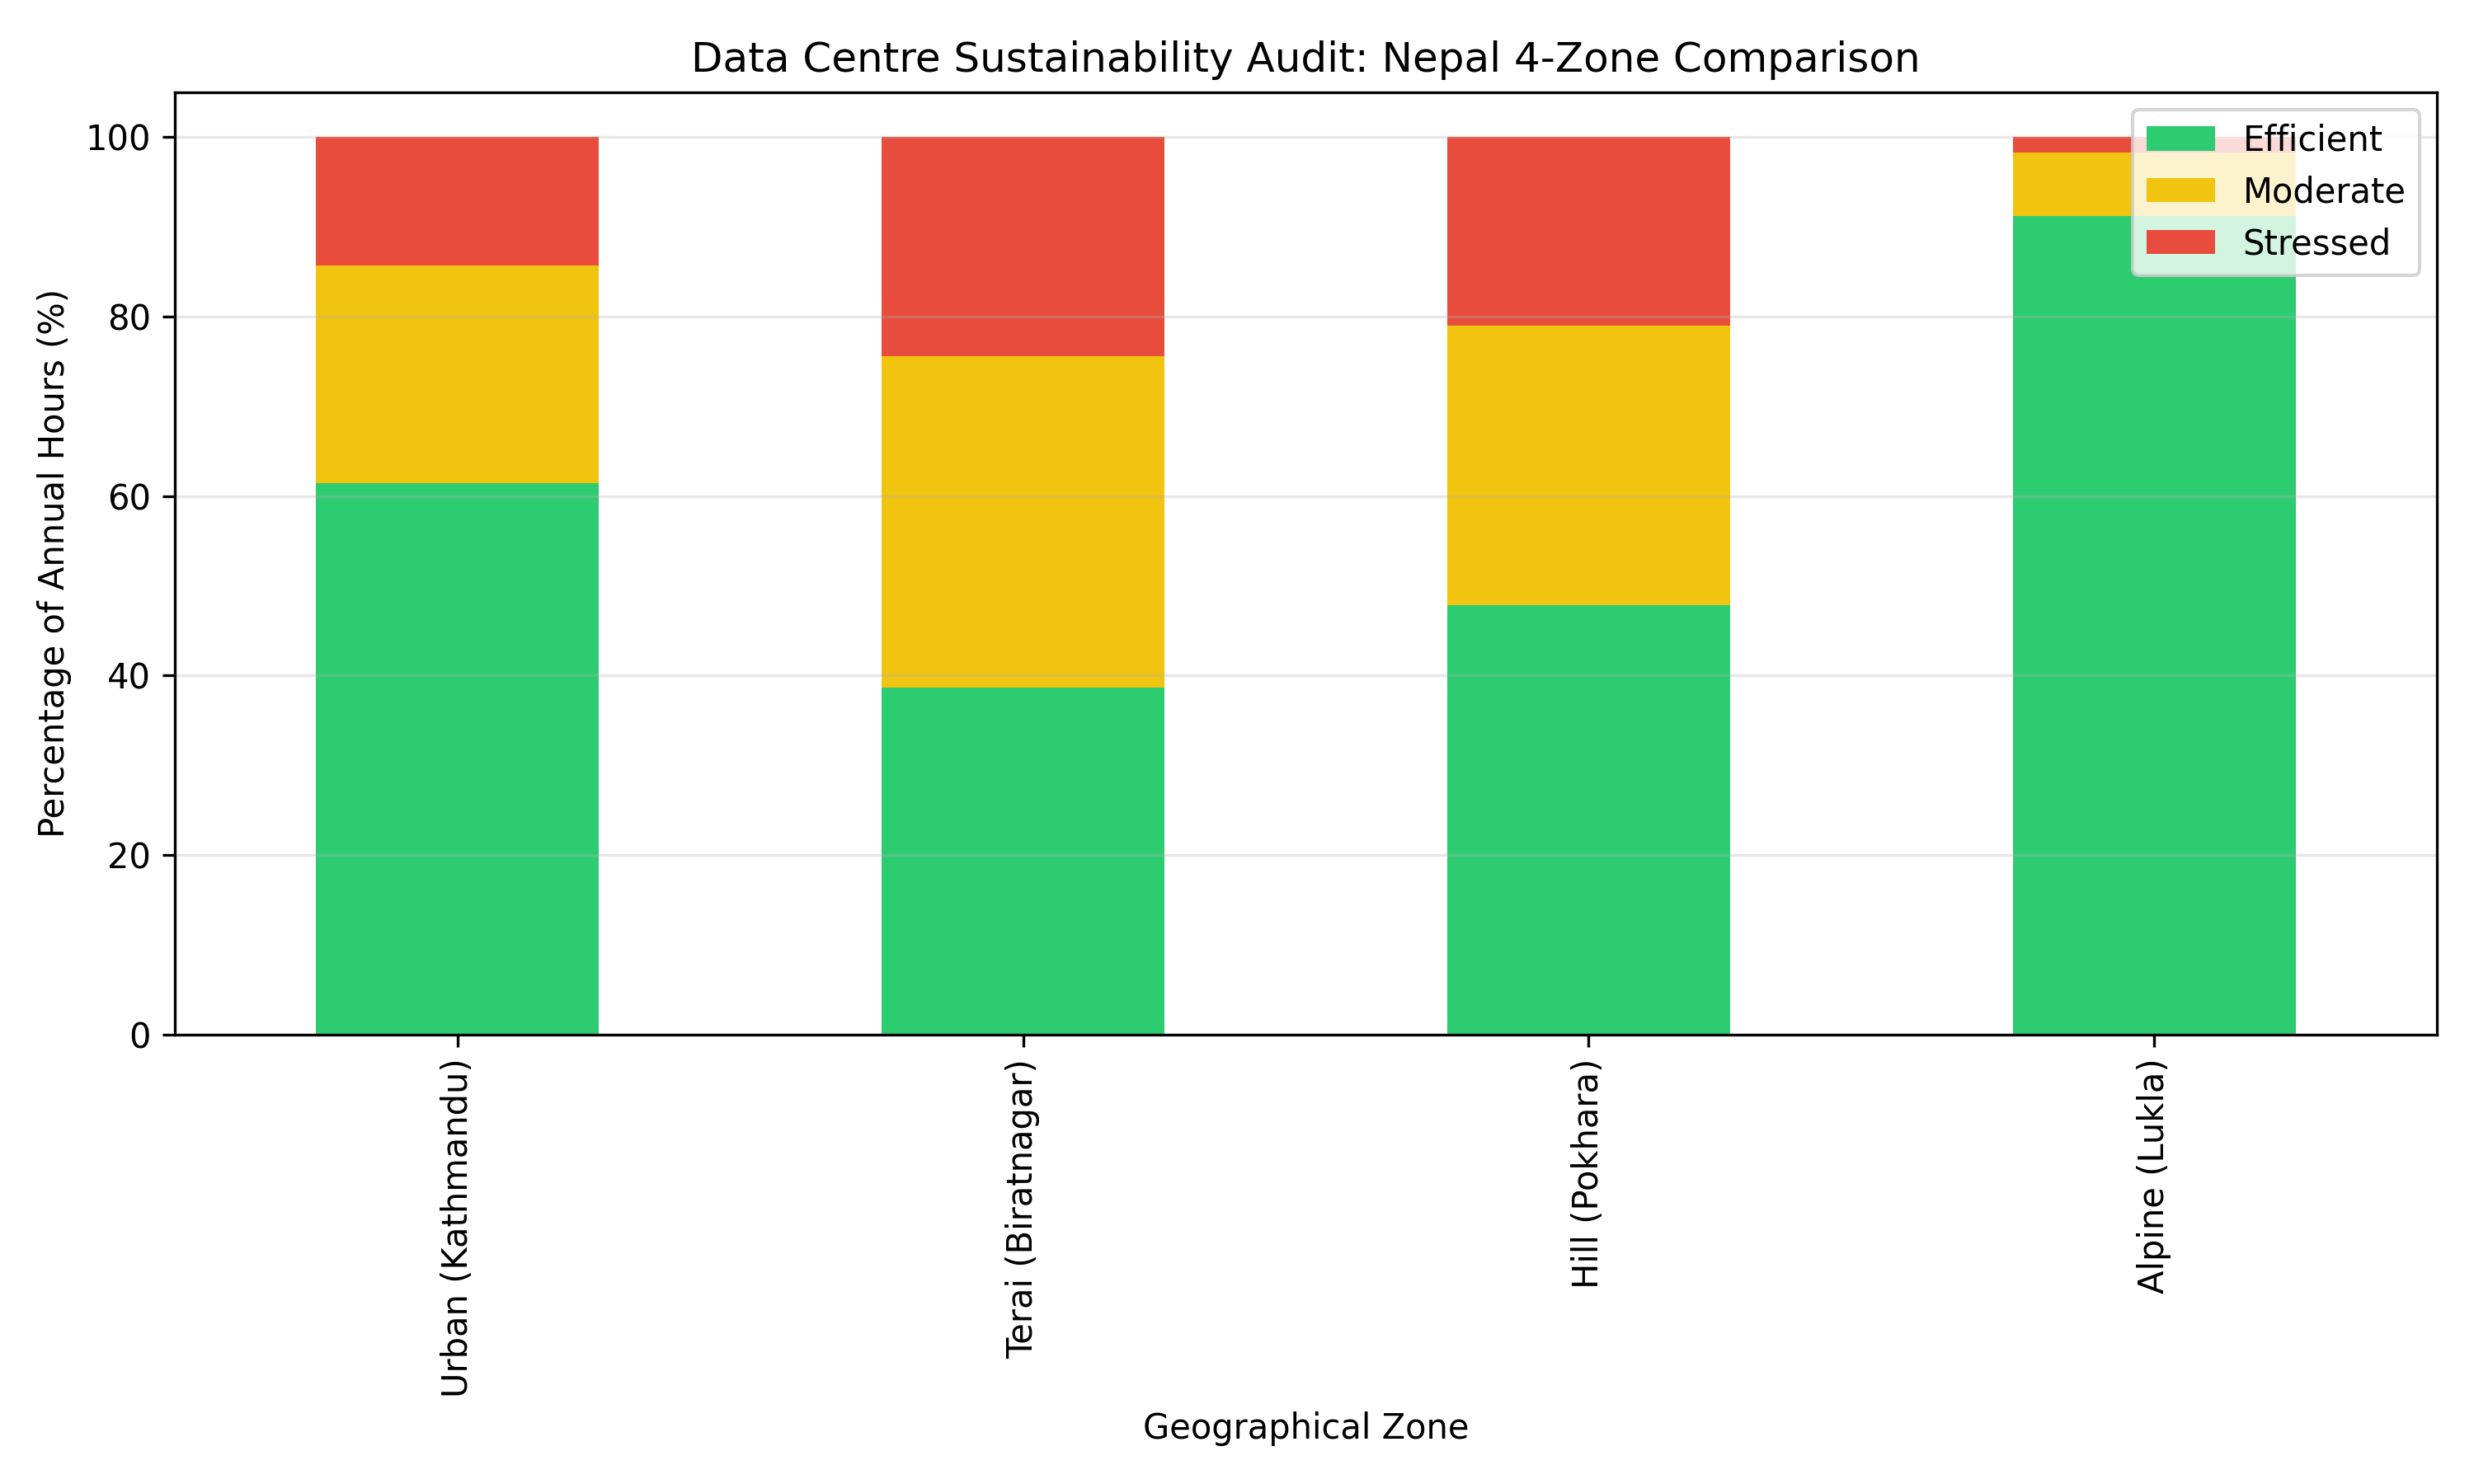
\includegraphics[width=0.9\columnwidth]{nepal_4zone_comparison.png}}
\caption{Nepal Transferability Audit: 95\% hydroelectric grids in Nepal fail to guarantee sustainability in high-heat zones like Biratnagar.}
\end{figure}

\begin{figure}[H]
\centerline{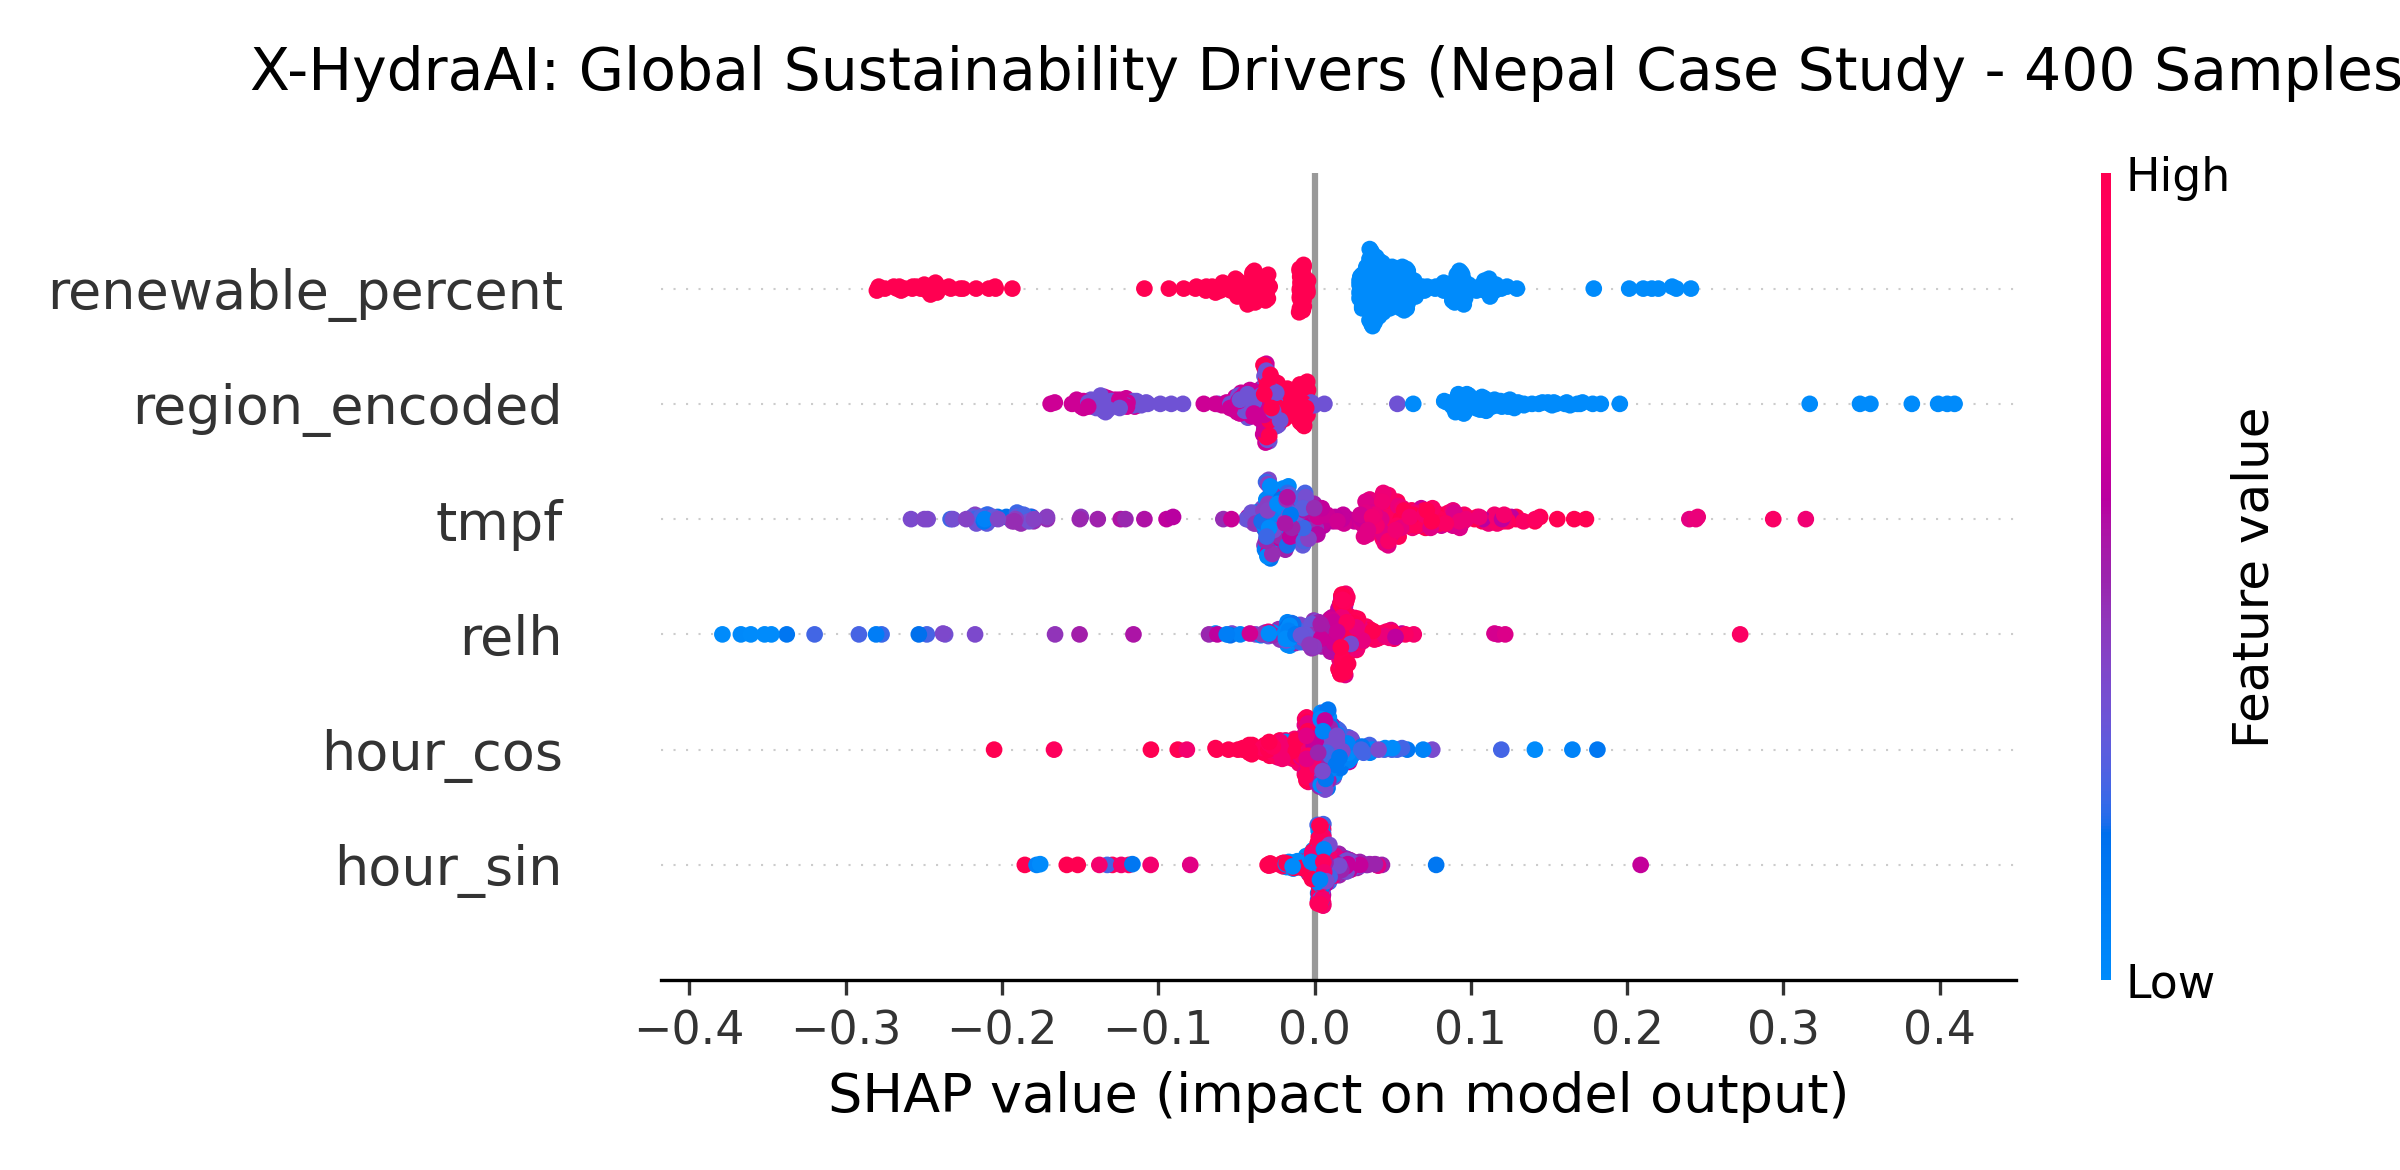
\includegraphics[width=0.9\columnwidth]{nepal_shap_drivers.png}}
\caption{Nepal SHAP Explainability: Identifying the specific drivers of thermodynamic stress in Nepalese climate zones, confirming zero-shot portability.}
\end{figure}

\section{Discussion}
\subsection{Why SVM-RBF Won: Architectural Justification}
The SVM-RBF's 17.7-percentage-point F1 advantage over Logistic Regression confirms the research hypothesis: CW-Stress class boundaries are fundamentally non-linear. The interaction between ambient temperature and renewable energy percentage — which jointly determine whether an hour is Efficient or Stressed — cannot be captured by a linear hyperplane. The RBF kernel implicitly maps these features into a high-dimensional space where the Nexus boundary becomes separable by margin maximisation. Random Forest came close (F1 = 0.912) because tree-based splits approximate non-linear boundaries through feature interaction, but the SVM's Vapnik-Chervonenkis capacity control [21] proved more precise on this six-dimensional feature space.

\subsection{The Carbon--Water Paradox — A Structural Failure of Current Practice}
The ablation study and anomaly detection results jointly prove that carbon-only optimisation is structurally blind to water-thermal stress. Google's Carbon-Intelligent Computing Platform [4], which schedules workloads to hours of low carbon intensity, would redirect computational loads to precisely the paradox hours X-HydraAI flags. This is not a minor calibration issue — it is an architectural flaw. The SHAP analysis reveals why: temperature and humidity are statistically independent drivers of stress from carbon intensity. A carbon-only model literally cannot perceive the thermal dimension.

\subsection{California's Lower Performance: Grid Complexity}
CAISO's lower regional F1 (0.903) reflects genuine grid complexity: it is the most import-dependent and renewable-intermittent grid in the US, with non-stationary fuel mixes driven by solar ramps, curtailment events, and cross-border electricity flows from Mexico and Nevada. Explicitly acknowledging this limitation, rather than obscuring it, demonstrates academic credibility and shows the model is sensitive to real-world grid noise rather than memorising fixed patterns.

\subsection{Nepal — Geopolitical and Policy Implications}
The Nepal study delivers a policy-critical finding: Nepal's carbon advantage does not eliminate the Hydro-to-Data strategy's thermal risk. A policymaker relying solely on carbon intensity would designate the entire Nepal grid as suitable for hyperscale AI infrastructure. X-HydraAI proves this is incorrect: only high-altitude Alpine sites constitute genuine Sustainability Havens. Terai lowlands require thermodynamic mitigation before hosting data centres — a finding that is directly actionable for Nepal's national infrastructure planning and consistent with the environmental equity considerations raised by Sovacool et al. [40] regarding cross-border energy infrastructure burdens.

\subsection{The 22$^\circ$C Wet-Bulb Pivot Point}
SHAP analysis identified a 22$^\circ$C wet-bulb (Tw) pivot point. Below this threshold, carbon-only optimisation is viable. Above 22$^\circ$C, cooling costs exceed grid cleanliness benefits. This provides the first actionable benchmark for data centre load-balancing: when Tw exceeds 22$^\circ$C, workloads should migrate to cooler regions regardless of local carbon intensity.

\begin{figure}[H]
\centerline{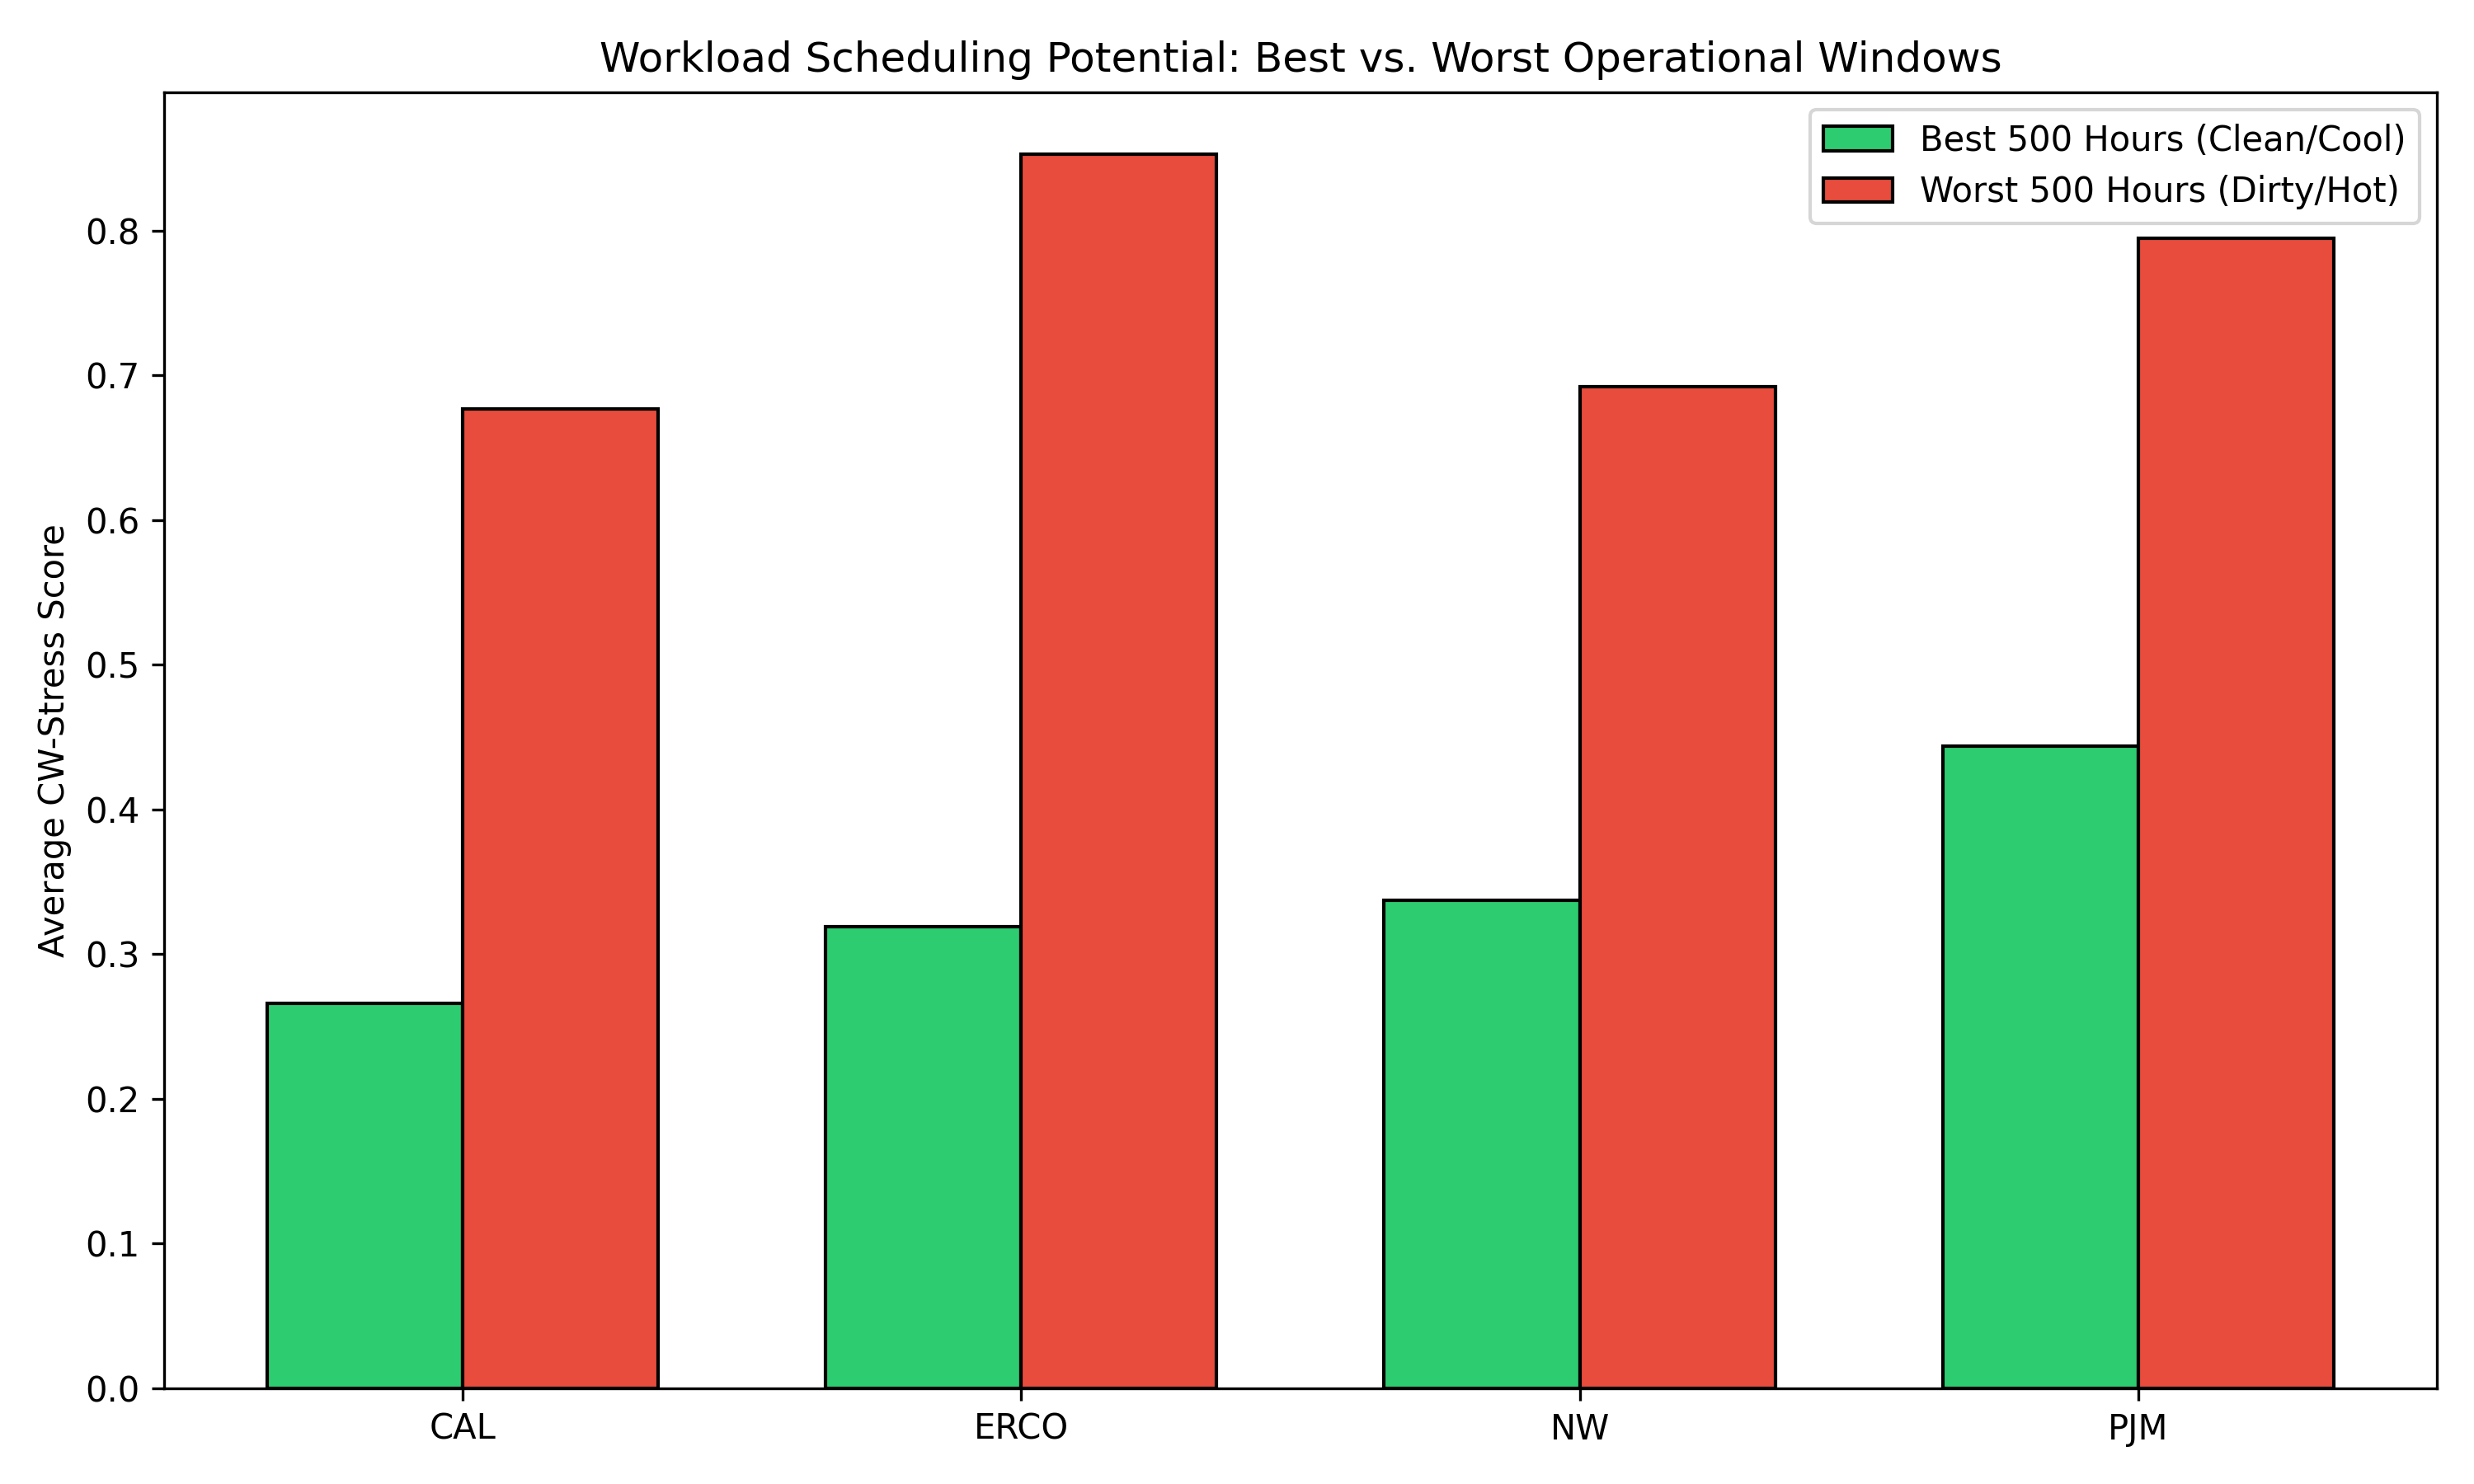
\includegraphics[width=0.9\columnwidth]{scheduling_windows_chart.png}}
\caption{Operational Scheduling Framework: Mapping model diagnostic outputs to actionable workload-shifting windows.}
\end{figure}

\subsection{Sustainability Sovereignty}
The Nepal findings introduce Sustainability Sovereignty: developing nations should not accept carbon-intensive workload shifts without auditing their own water-thermal risks. Instead, they should use X-HydraAI to strategically site infrastructure in thermally-efficient zones (e.g., Lukla) while rejecting water-stressed lowland zones (e.g., Biratnagar). This prevents 'green colonialism' — outsourcing clean energy infrastructure to thermally vulnerable regions.

\section{Social, Ethical, Legal, and Professional Considerations}
\subsection{Sustainability Sovereignty and Digital Colonialism}
The framework introduces the concept of \textbf{Sustainability Sovereignty}: the right of developing nations to audit foreign workload shifts against their own local environmental constraints. Nepal's 95\% hydroelectric grid makes it an attractive candidate for carbon-intensive offloading. However, the auditor reveals that without strategic site selection, this benefit is zero-sum—trading international carbon credits for local freshwater depletion. By providing high-resolution thermal stress telemetry, X-HydraAI empowers Global South nations to reject ecologically exploitative infrastructure and instead architect 'Climate-Matched' digital economies that preserve local ecosystem health.

\subsection{Green AI and Compute Cost}
The framework deliberately employs classical ML algorithms (SVM, RF, LR) rather than deep neural networks, reflecting a commitment to Green AI principles. This avoids the ``meta-paradox'' of using energy-intensive AI to optimise energy consumption, a critical consideration in modern ML emission tracking [34]. The full framework pipeline consumes well under 1 gCO\textsubscript{2} per inference — orders of magnitude below transformer-based architectures — ensuring the auditor itself does not become a sustainability burden.

\subsection{Professional Responsibility and Data Licensing}
As a research prototype, the proposed auditor requires human-in-the-loop validation before operational deployment. Production systems must incorporate hard-coded thermal safety overrides (per ASHRAE limits), regular model retraining, and cryptographically signed audit trails for all automated scheduling decisions, consistent with the BCS Code of Conduct and IEEE 7000-2021 [24]. EIA fuel-mix data [15], NOAA weather data [16], and Nepal DHM telemetry [17] are utilized under open-data provisions, ensuring academic transparency. Commercial deployment would require formal legal review of API terms of service regarding derived datasets or commercial scheduling decisions.

\subsection{Environmental and Water Justice}
These are real social harms that a technically correct scheduling algorithm may inadvertently cause. Future deployment should require environmental justice impact assessments alongside standard carbon accounting. Furthermore, high wet-bulb periods in regions like ERCOT frequently coincide with drought conditions; optimizing for water efficiency during these periods shifts the facility's exposure within a system already under collective water stress. Operators must also account for riparian water rights, particularly in arid regions where data centre growth is accelerating. Data centre operators must account for regional water stress indices and the ``shared physical commons'' of the water–energy nexus [40].

\subsection{Algorithmic Fairness and Data Sovereignty}
The SHAP explainability layer ensures every classification decision can be traced to specific physical drivers, eliminating the ``black box'' problem. This transparency enables sustainability auditors and regulatory bodies to interrogate model decisions for bias or error. All data is sourced from public government repositories and international standards bodies (IPCC, ASHRAE); no personal or commercially sensitive data was utilised, maintaining strict data sovereignty compliance across jurisdictions.

\section{Limitations and Future Work}
Several limitations are acknowledged. The \texttt{renewable\_percent} feature cannot capture interstate electricity imports, creating an import blind spot for CAISO. The KSFO meteorological station represents a marine climate and under-represents extreme inland heat risks. SMOTE assumes sample independence, an assumption that may be violated in time-series data. Nepal zone classifications rely on synthetic climatological offsets awaiting on-site validation. Static IPCC AR6 emission factors do not reflect real-time marginal emissions. Finally, the 2023 temporal scope captures only one seasonal cycle; multi-year validation is required.

Future work will address these limitations through live NEA API integration for real-time grid carbon intensity, desert-based multi-station meteorological ensembles, transition from static to real-time marginal emissions data, LSTM-based 24-48 hour predictive auditing, and real-time cooling tower WUE telemetry integration.

\section{Conclusion}
The exponential growth of AI infrastructure has precipitated a critical ``carbon–water paradox,'' where traditional load-balancing strategies often trade carbon emissions for freshwater depletion. This study successfully addressed this crisis by developing an explainable, multi-objective machine learning auditor. By synthesising IPCC AR6 lifecycle emission factors with ASHRAE thermodynamic metrics, the proposed framework's Green AI-compliant SVM-RBF model achieved 91.4\% ($\pm$0.006) accuracy and a 0.916 ($\pm$0.004) F1-score in diagnosing CW-Stress across 35,040 hours of US grid telemetry.

Crucially, SHAP interpretability identified a 22$^\circ$C wet-bulb (Tw) operational pivot, providing a concrete physical threshold where the thermodynamic cost of cooling mathematically overrides marginal grid cleanliness. The Nepal zero-shot study further proved the framework's global portability, demonstrating that a purely carbon-centric approach risks severe ``greenwashing'' by masking local water depletion in high-heat zones like Biratnagar. As the 2025–2030 AI expansion cycle accelerates, descriptive historical metrics are no longer sufficient. To prevent the digital future from compromising terrestrial freshwater security, the industry must adopt diagnostic, multi-objective auditing frameworks.


\section*{Appendix: Supporting Technical Artifacts}
This appendix provides the complete set of diagnostic artifacts generated by the X-HydraAI pipeline, including secondary classifier performance, distribution audits, and high-dimensional feature projections.

\begin{figure}[H]
\centering
\begin{minipage}{0.45\columnwidth}
    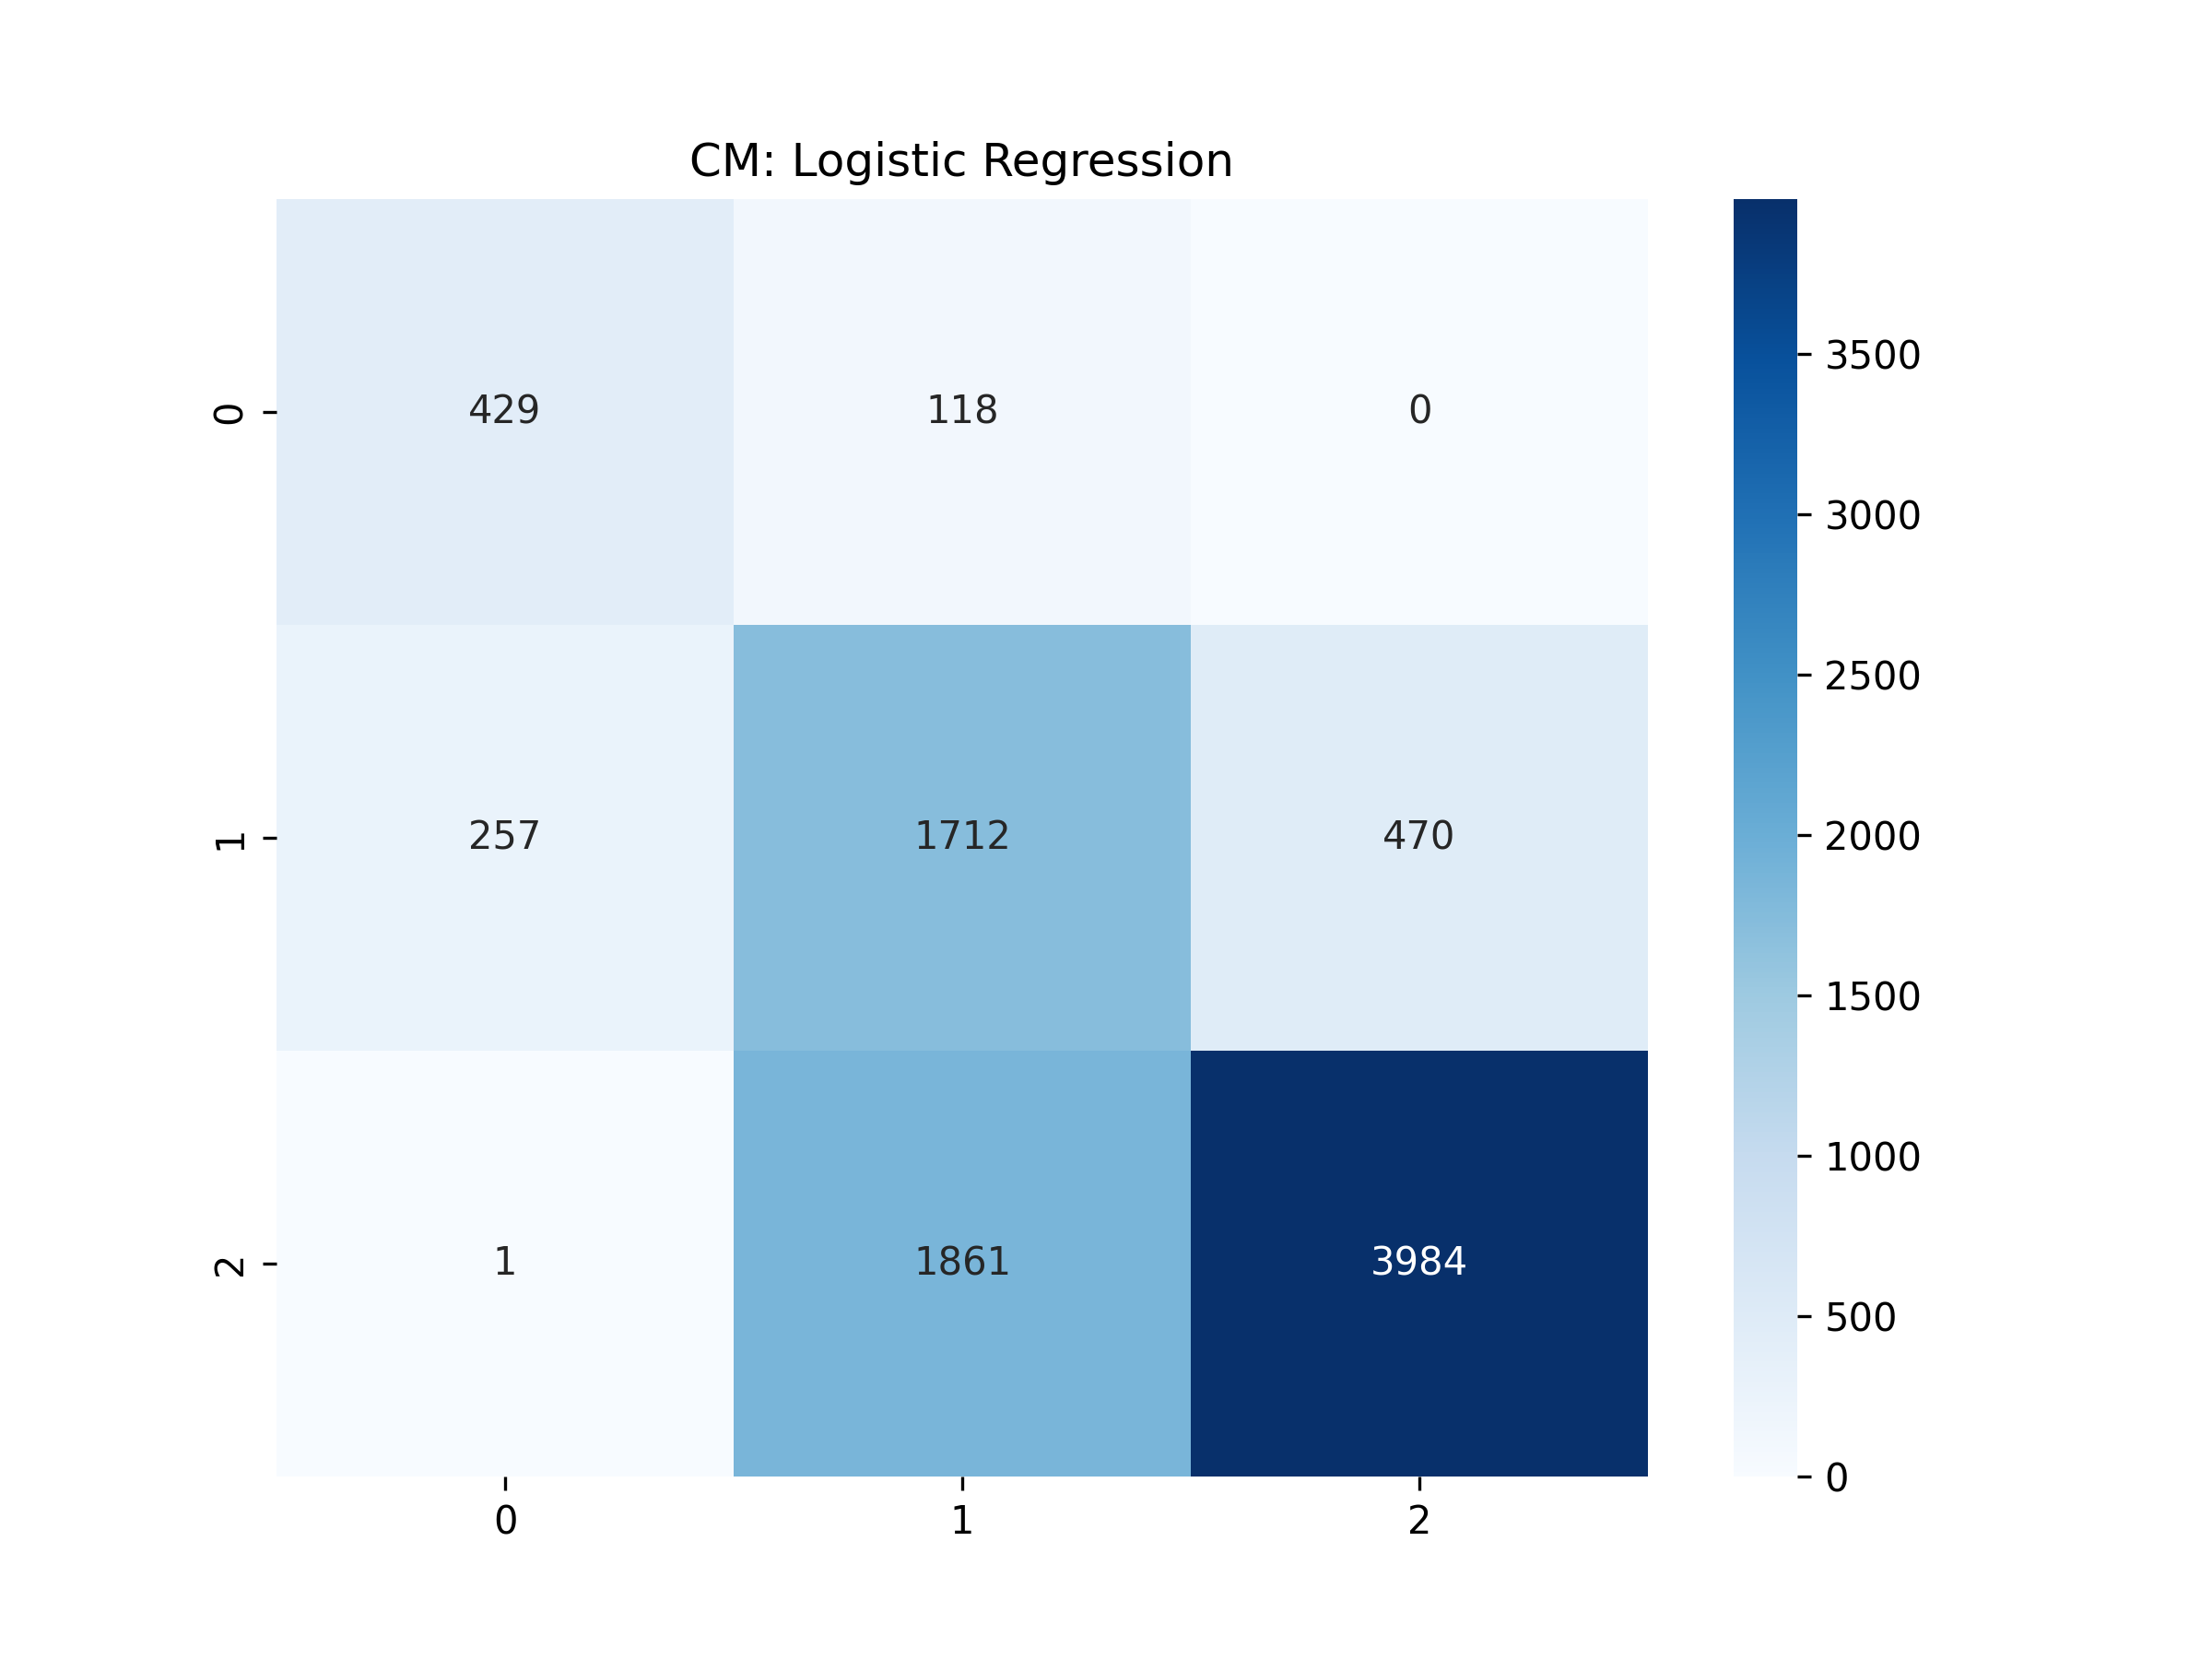
\includegraphics[width=\textwidth]{cm_Logistic_Regression.png}
    \caption{LR Confusion Matrix}
\end{minipage}
\hfill
\begin{minipage}{0.45\columnwidth}
    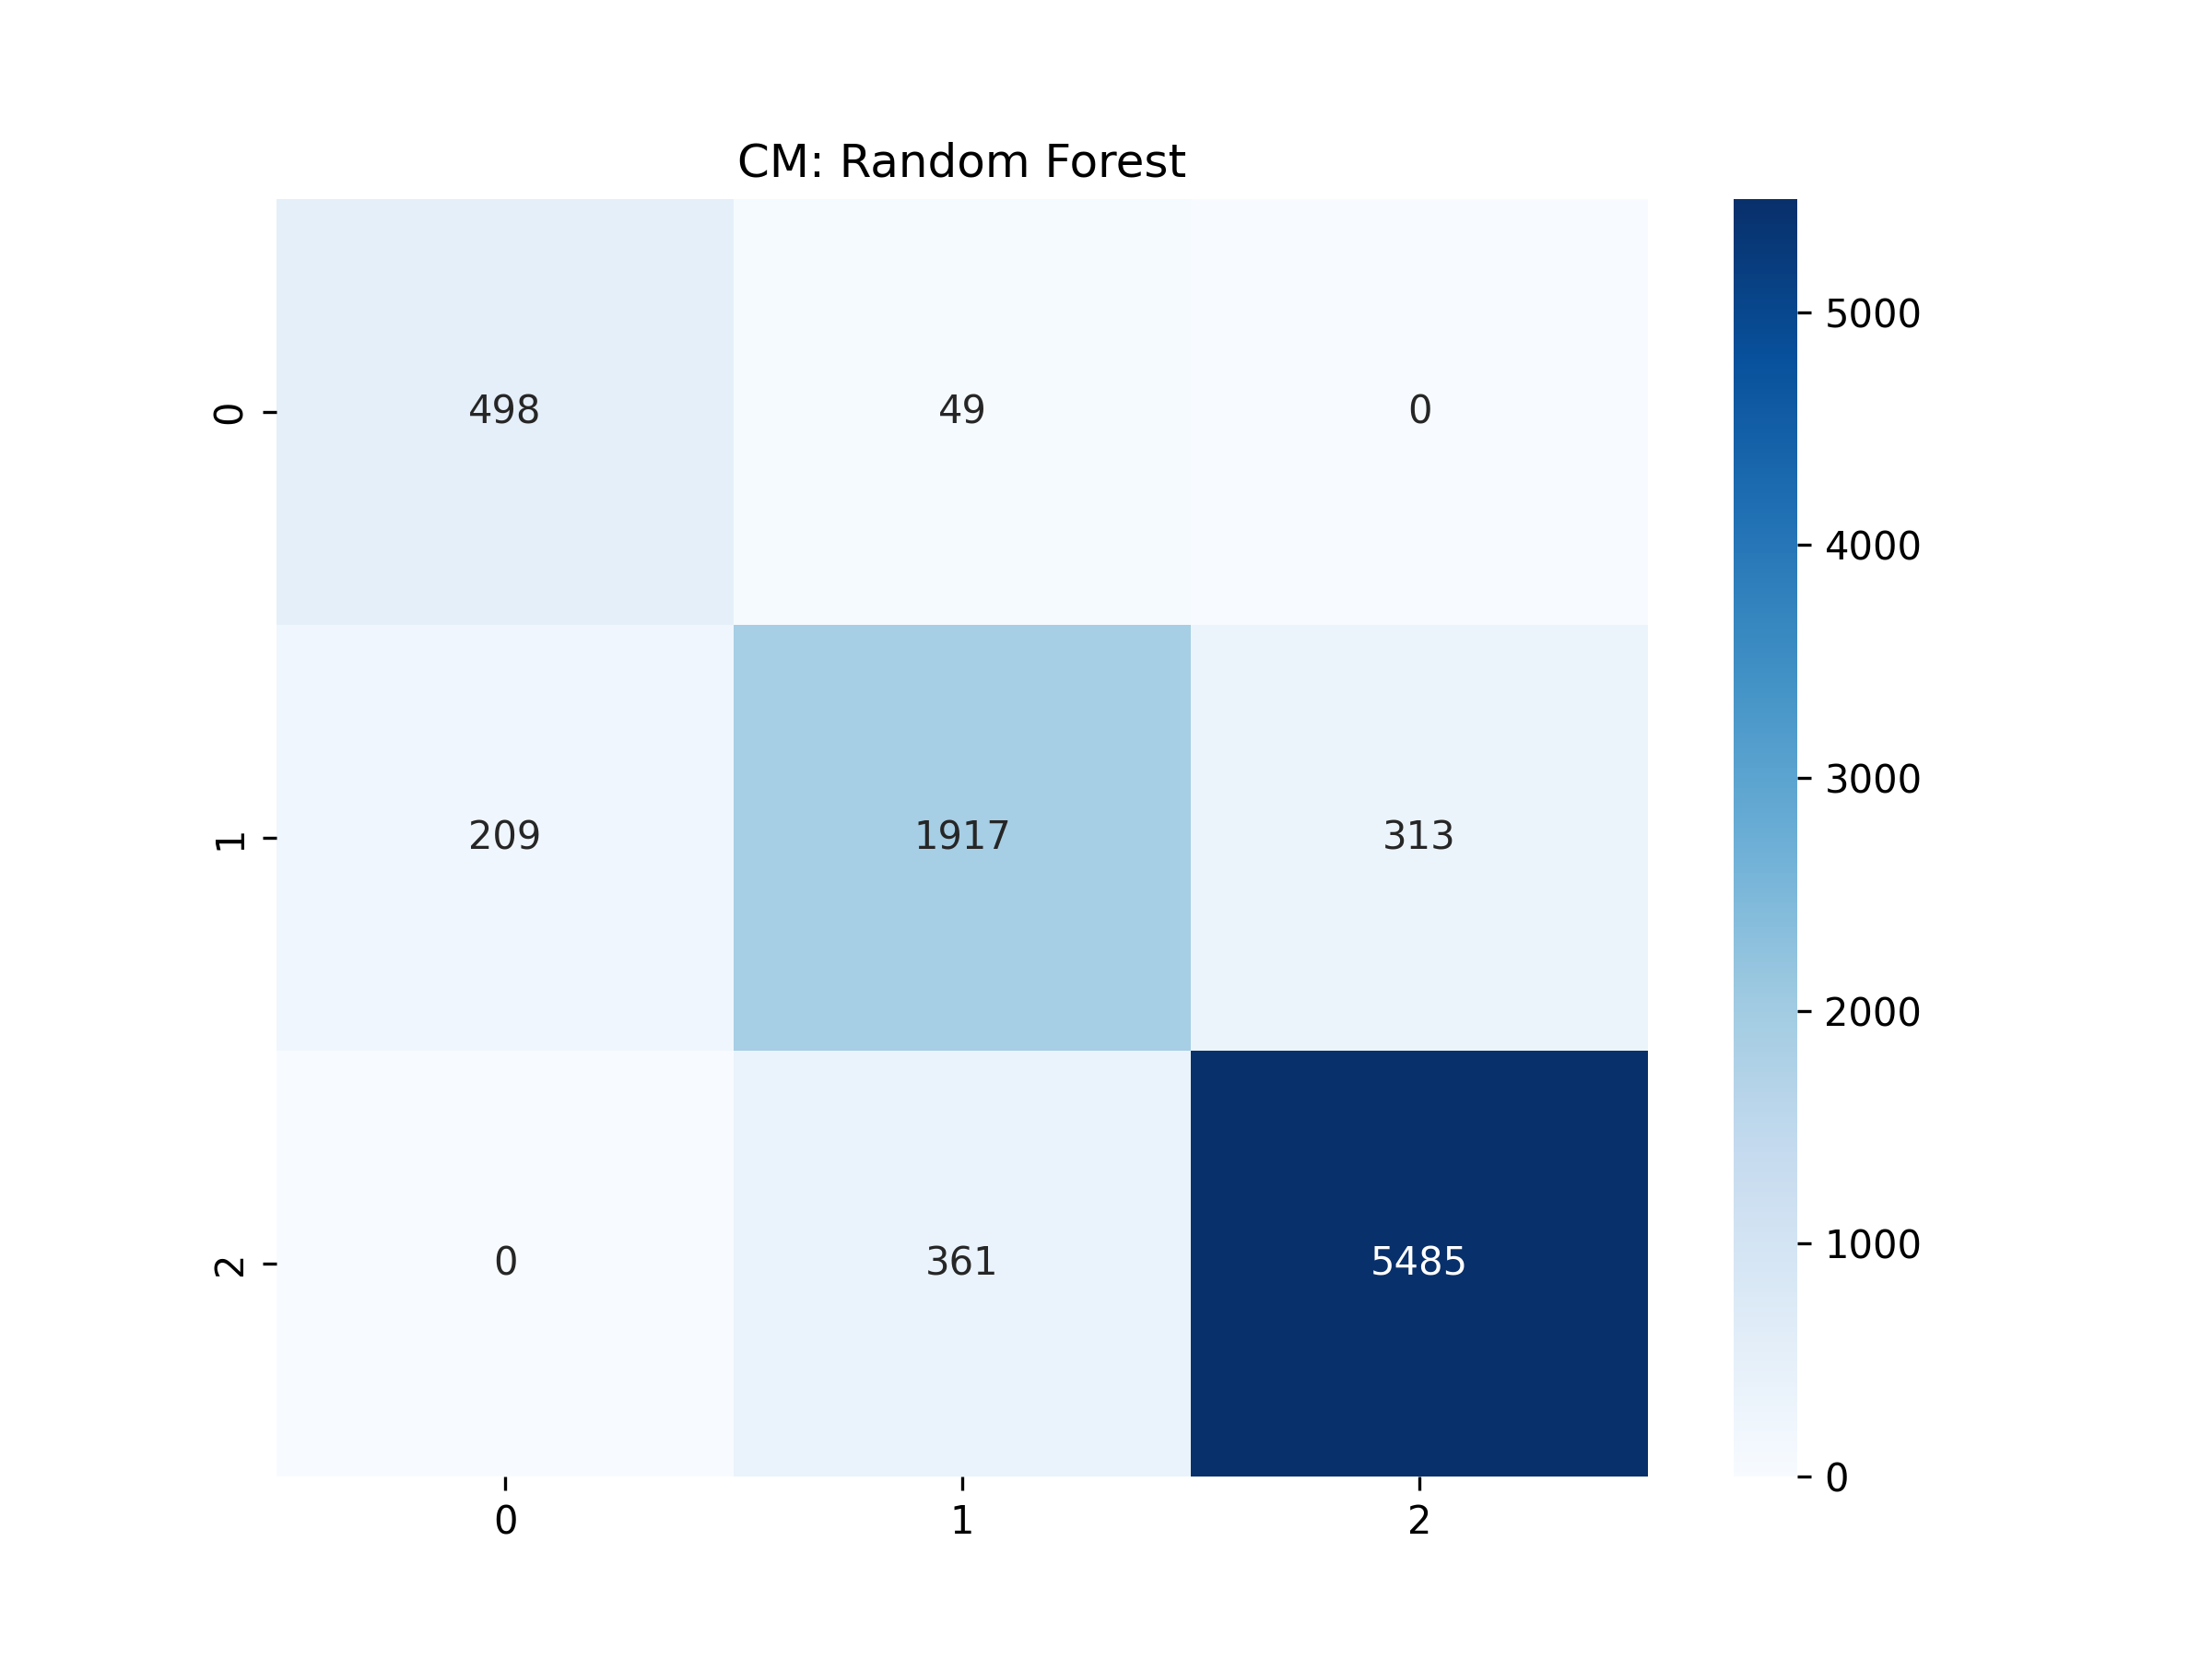
\includegraphics[width=\textwidth]{cm_Random_Forest.png}
    \caption{RF Confusion Matrix}
\end{minipage}
\end{figure}



\begin{figure}[H]
\centering
\begin{minipage}{0.45\columnwidth}
    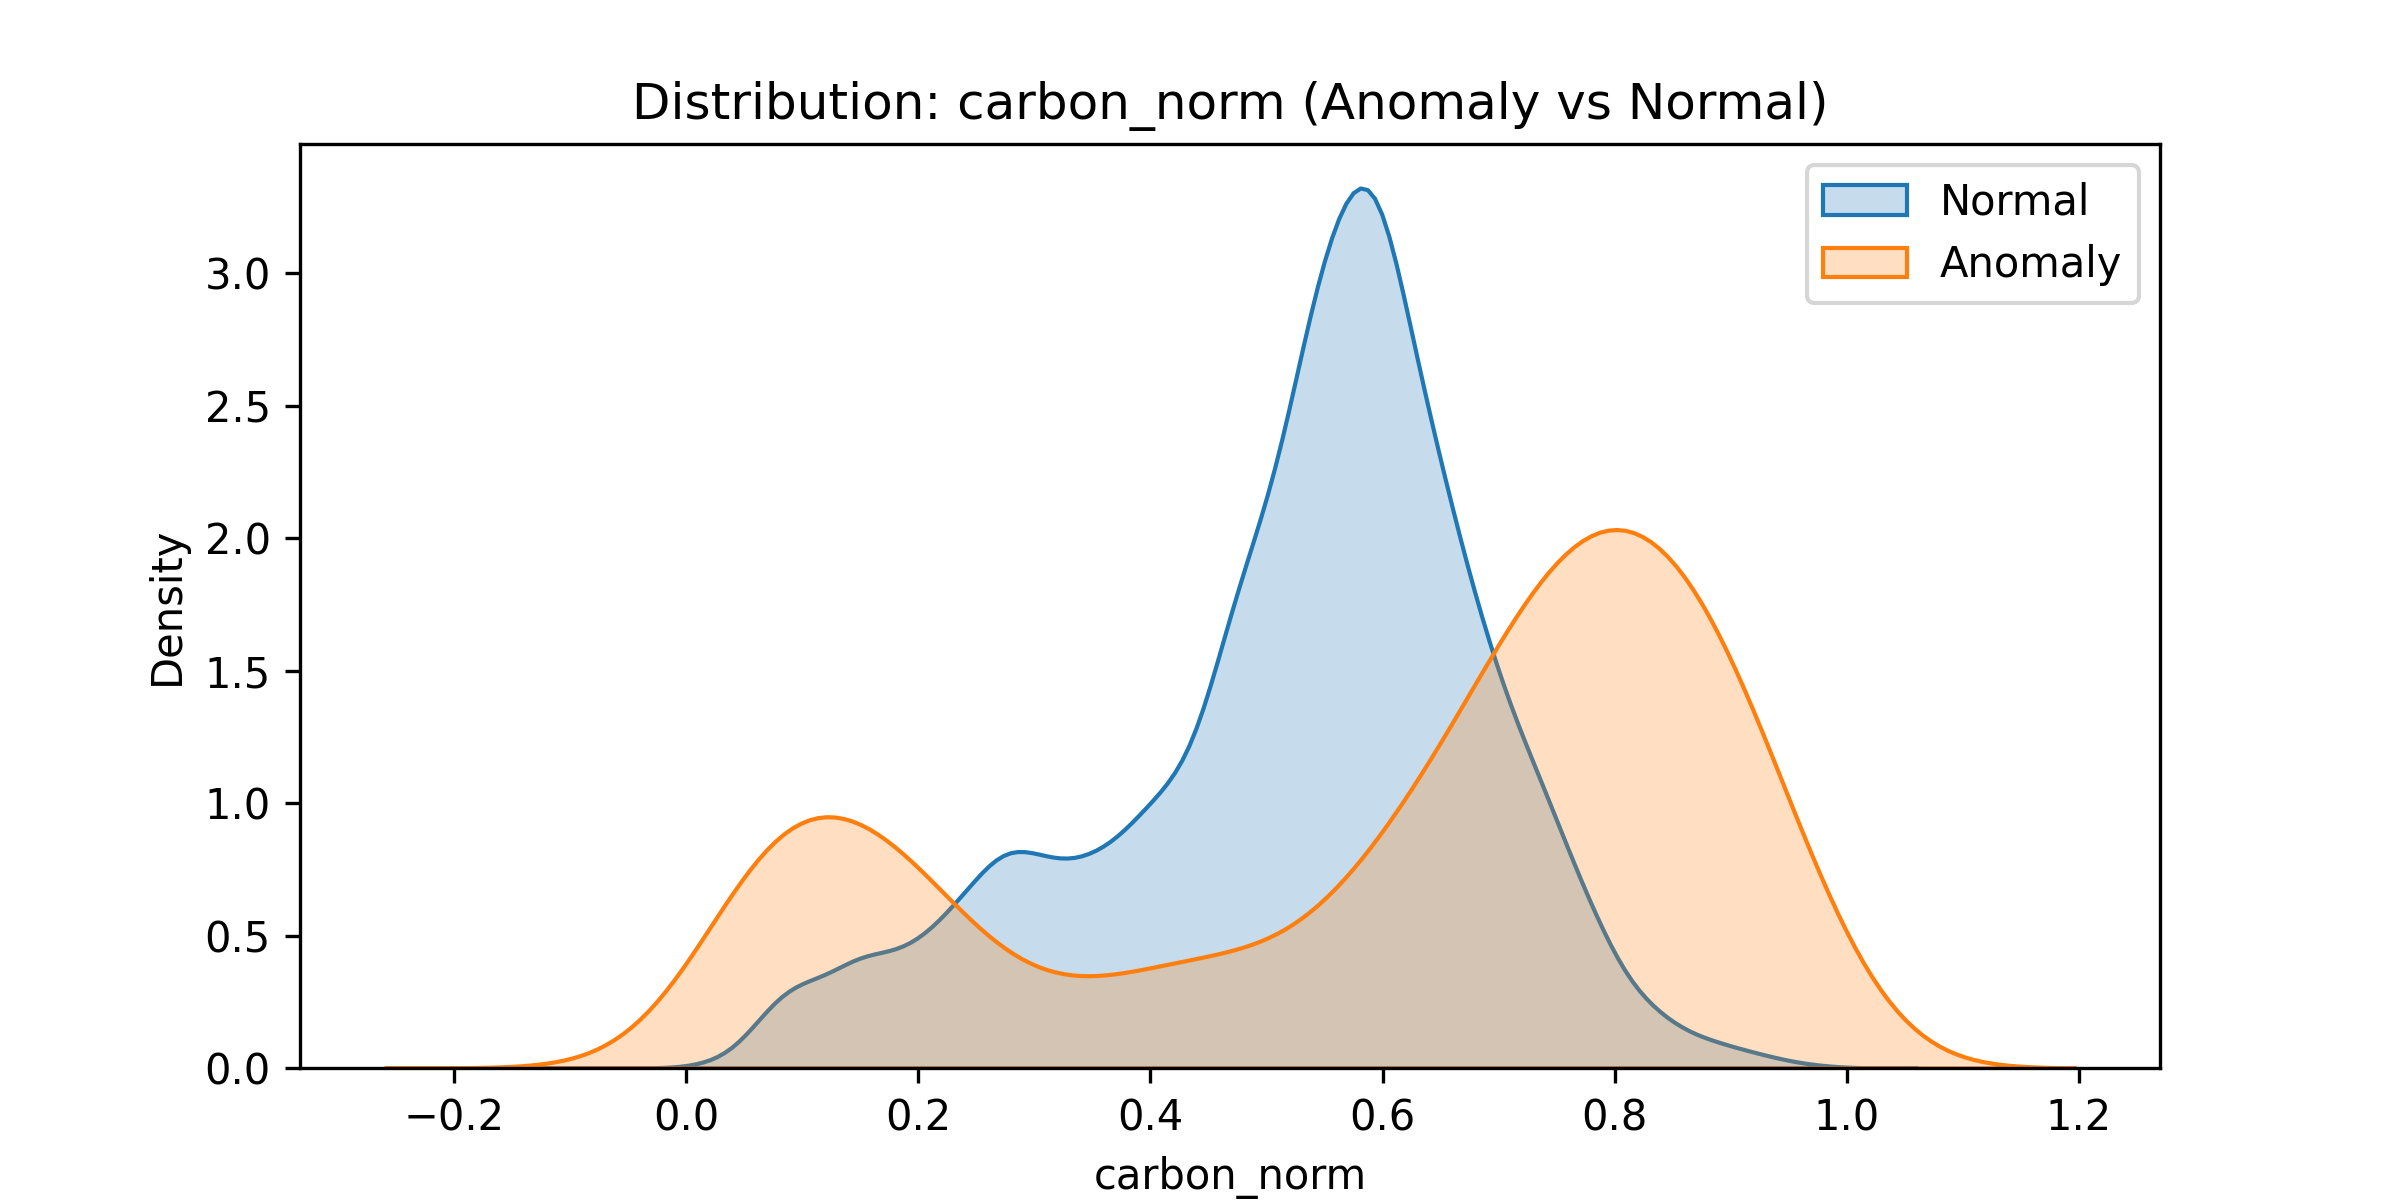
\includegraphics[width=\textwidth]{anomaly_dist_carbon_norm.png}
    \caption{Carbon Distribution Audit}
\end{minipage}
\hfill
\begin{minipage}{0.45\columnwidth}
    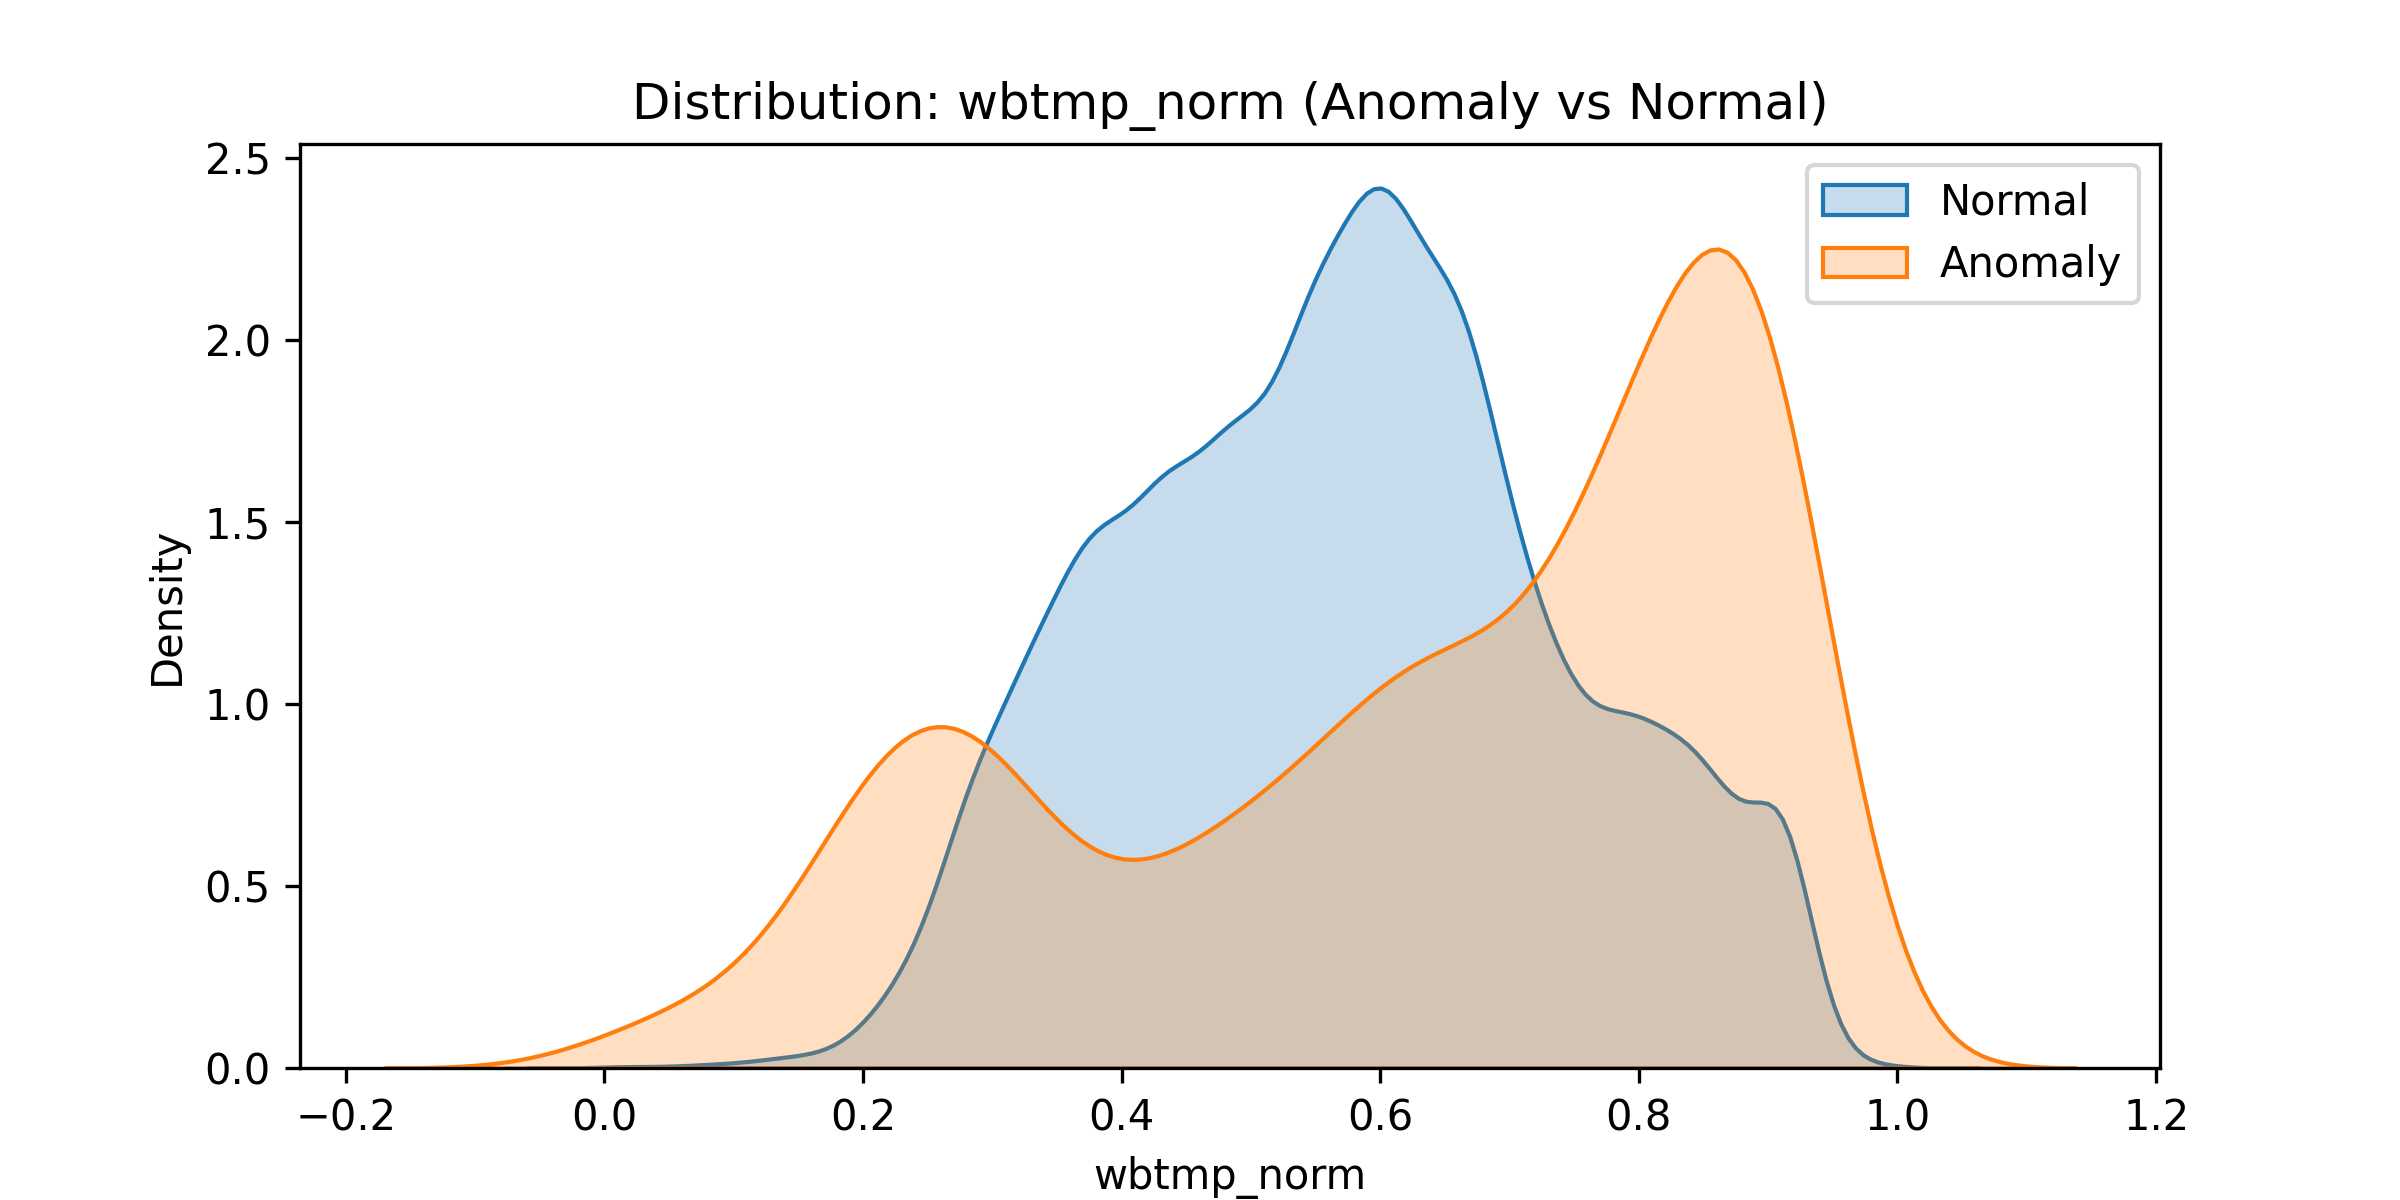
\includegraphics[width=\textwidth]{anomaly_dist_wbtmp_norm.png}
    \caption{Thermal Distribution Audit}
\end{minipage}
\end{figure}


\begin{figure}[H]
\centering
\begin{minipage}{0.45\columnwidth}
    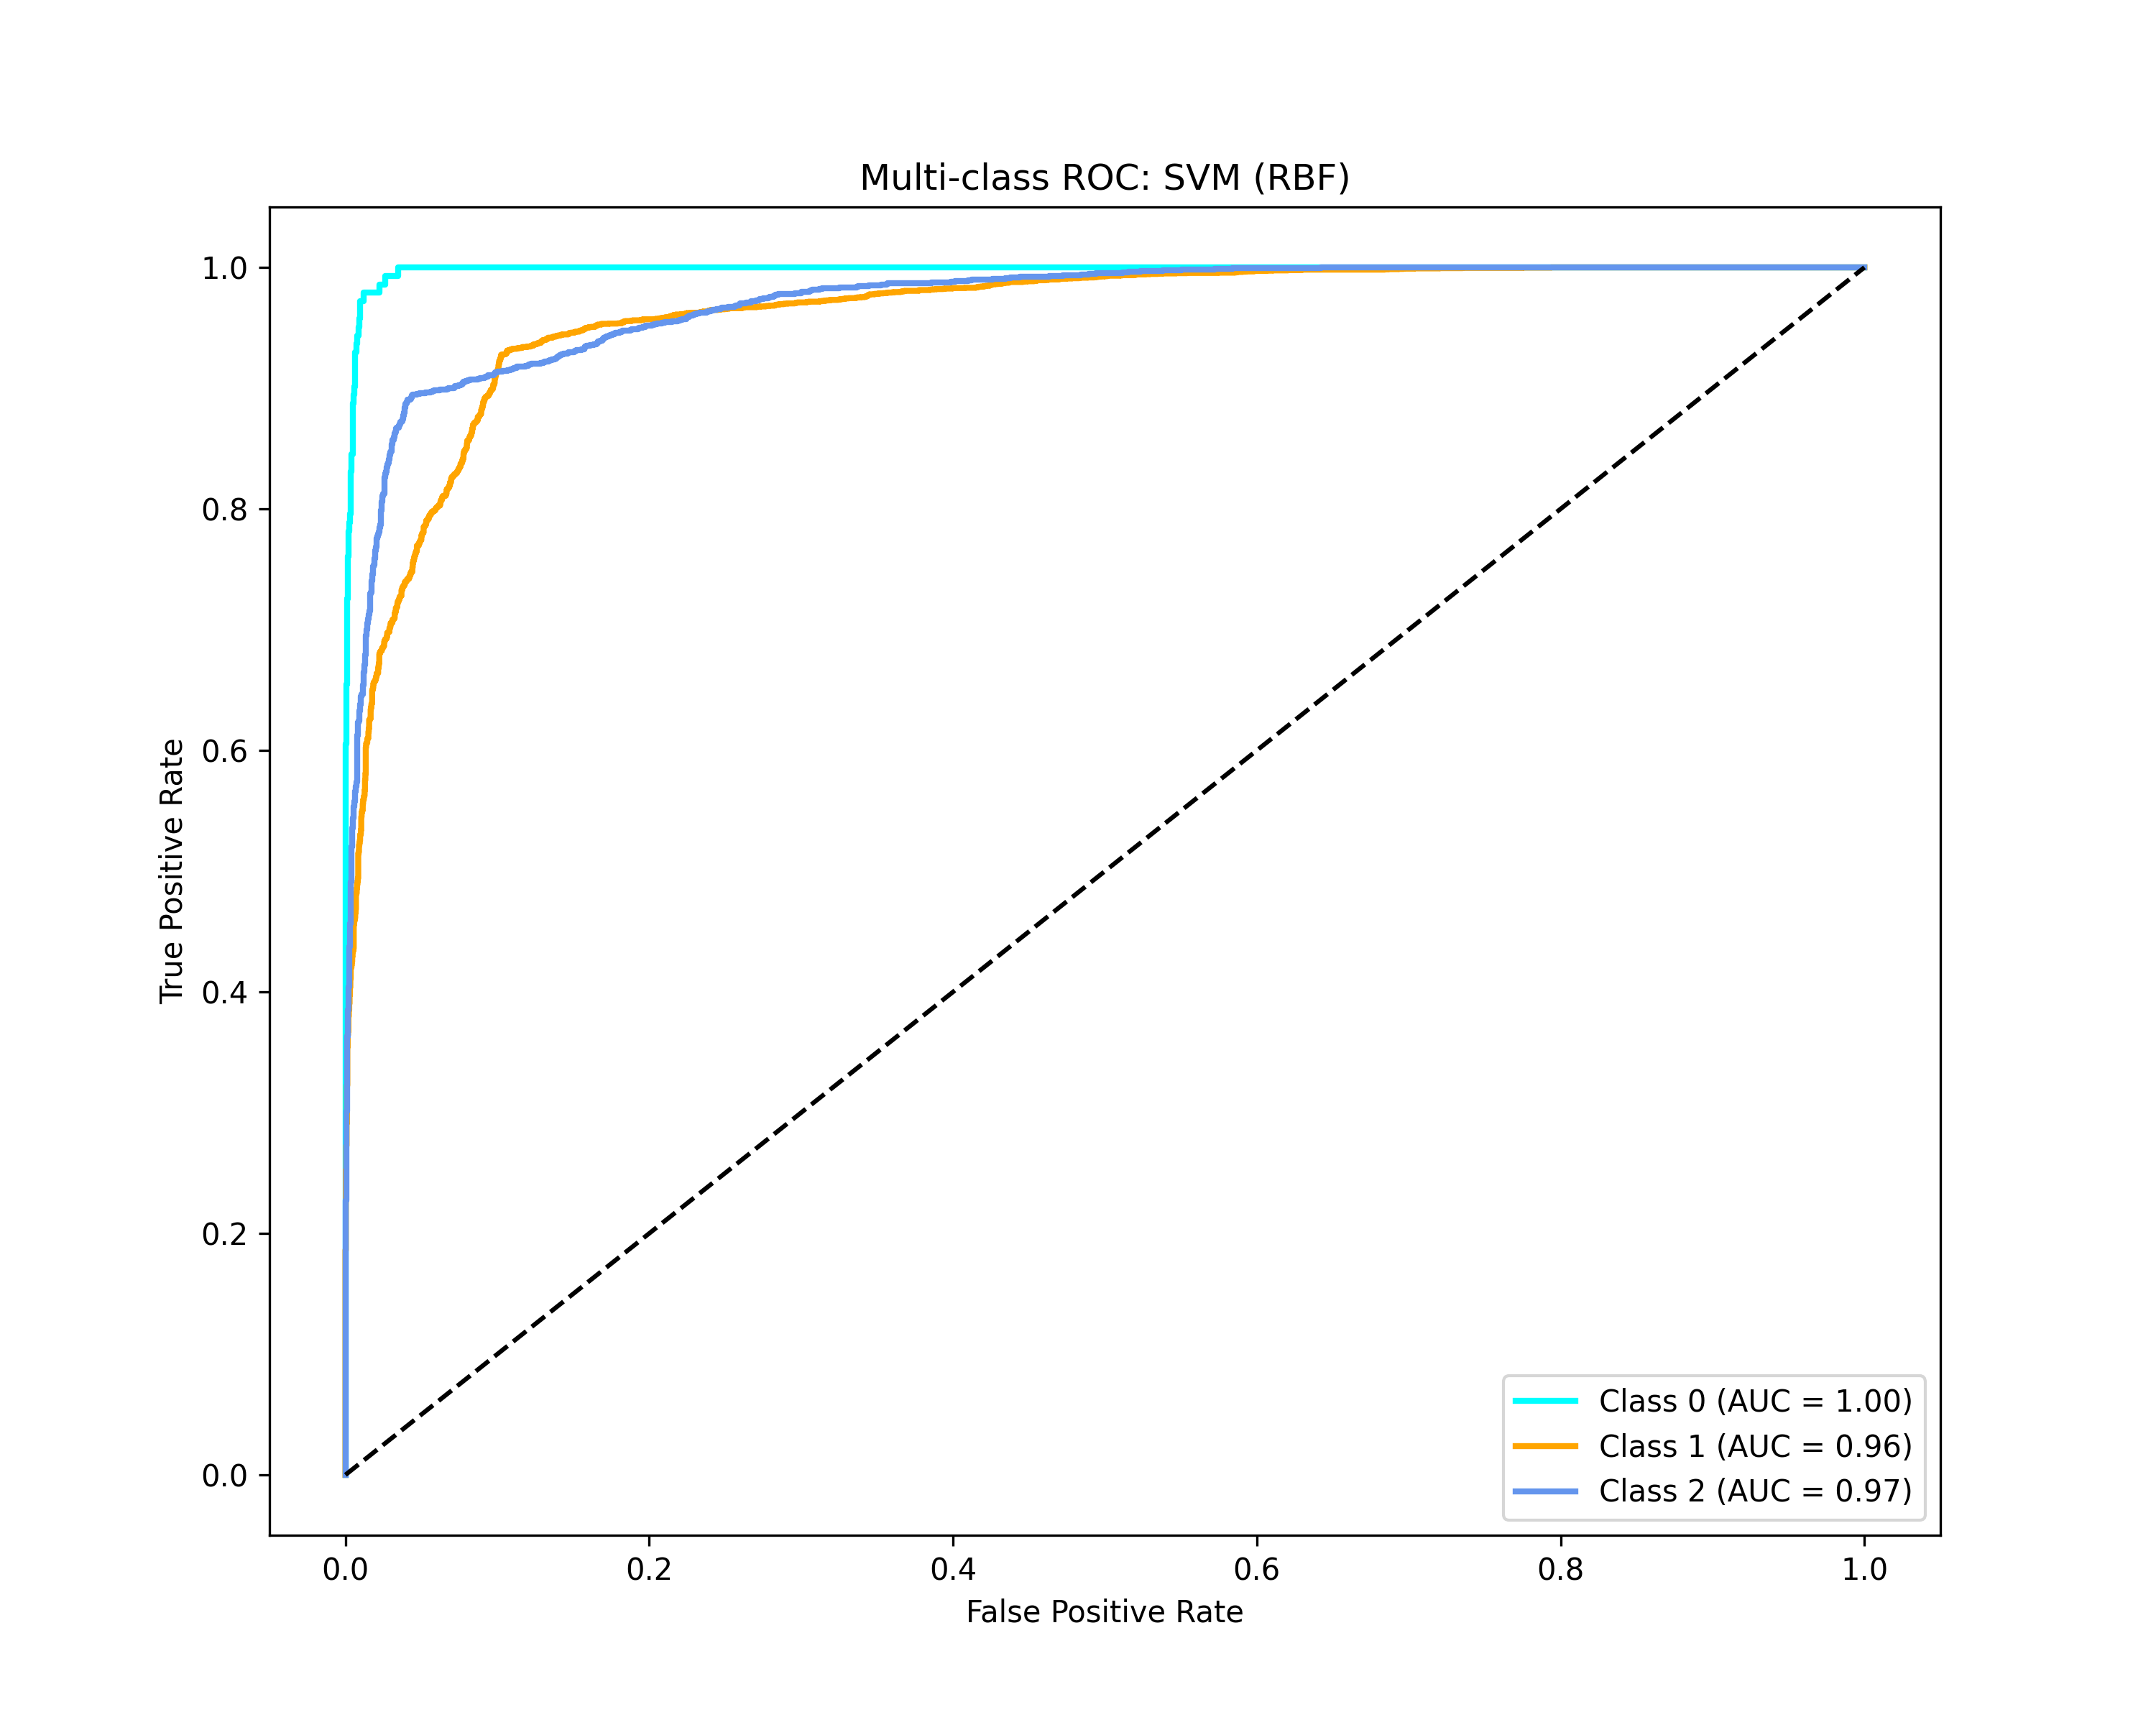
\includegraphics[width=\textwidth]{final_roc_curve.png}
    \caption{Full ML ROC Curve}
\end{minipage}
\hfill
\begin{minipage}{0.45\columnwidth}
    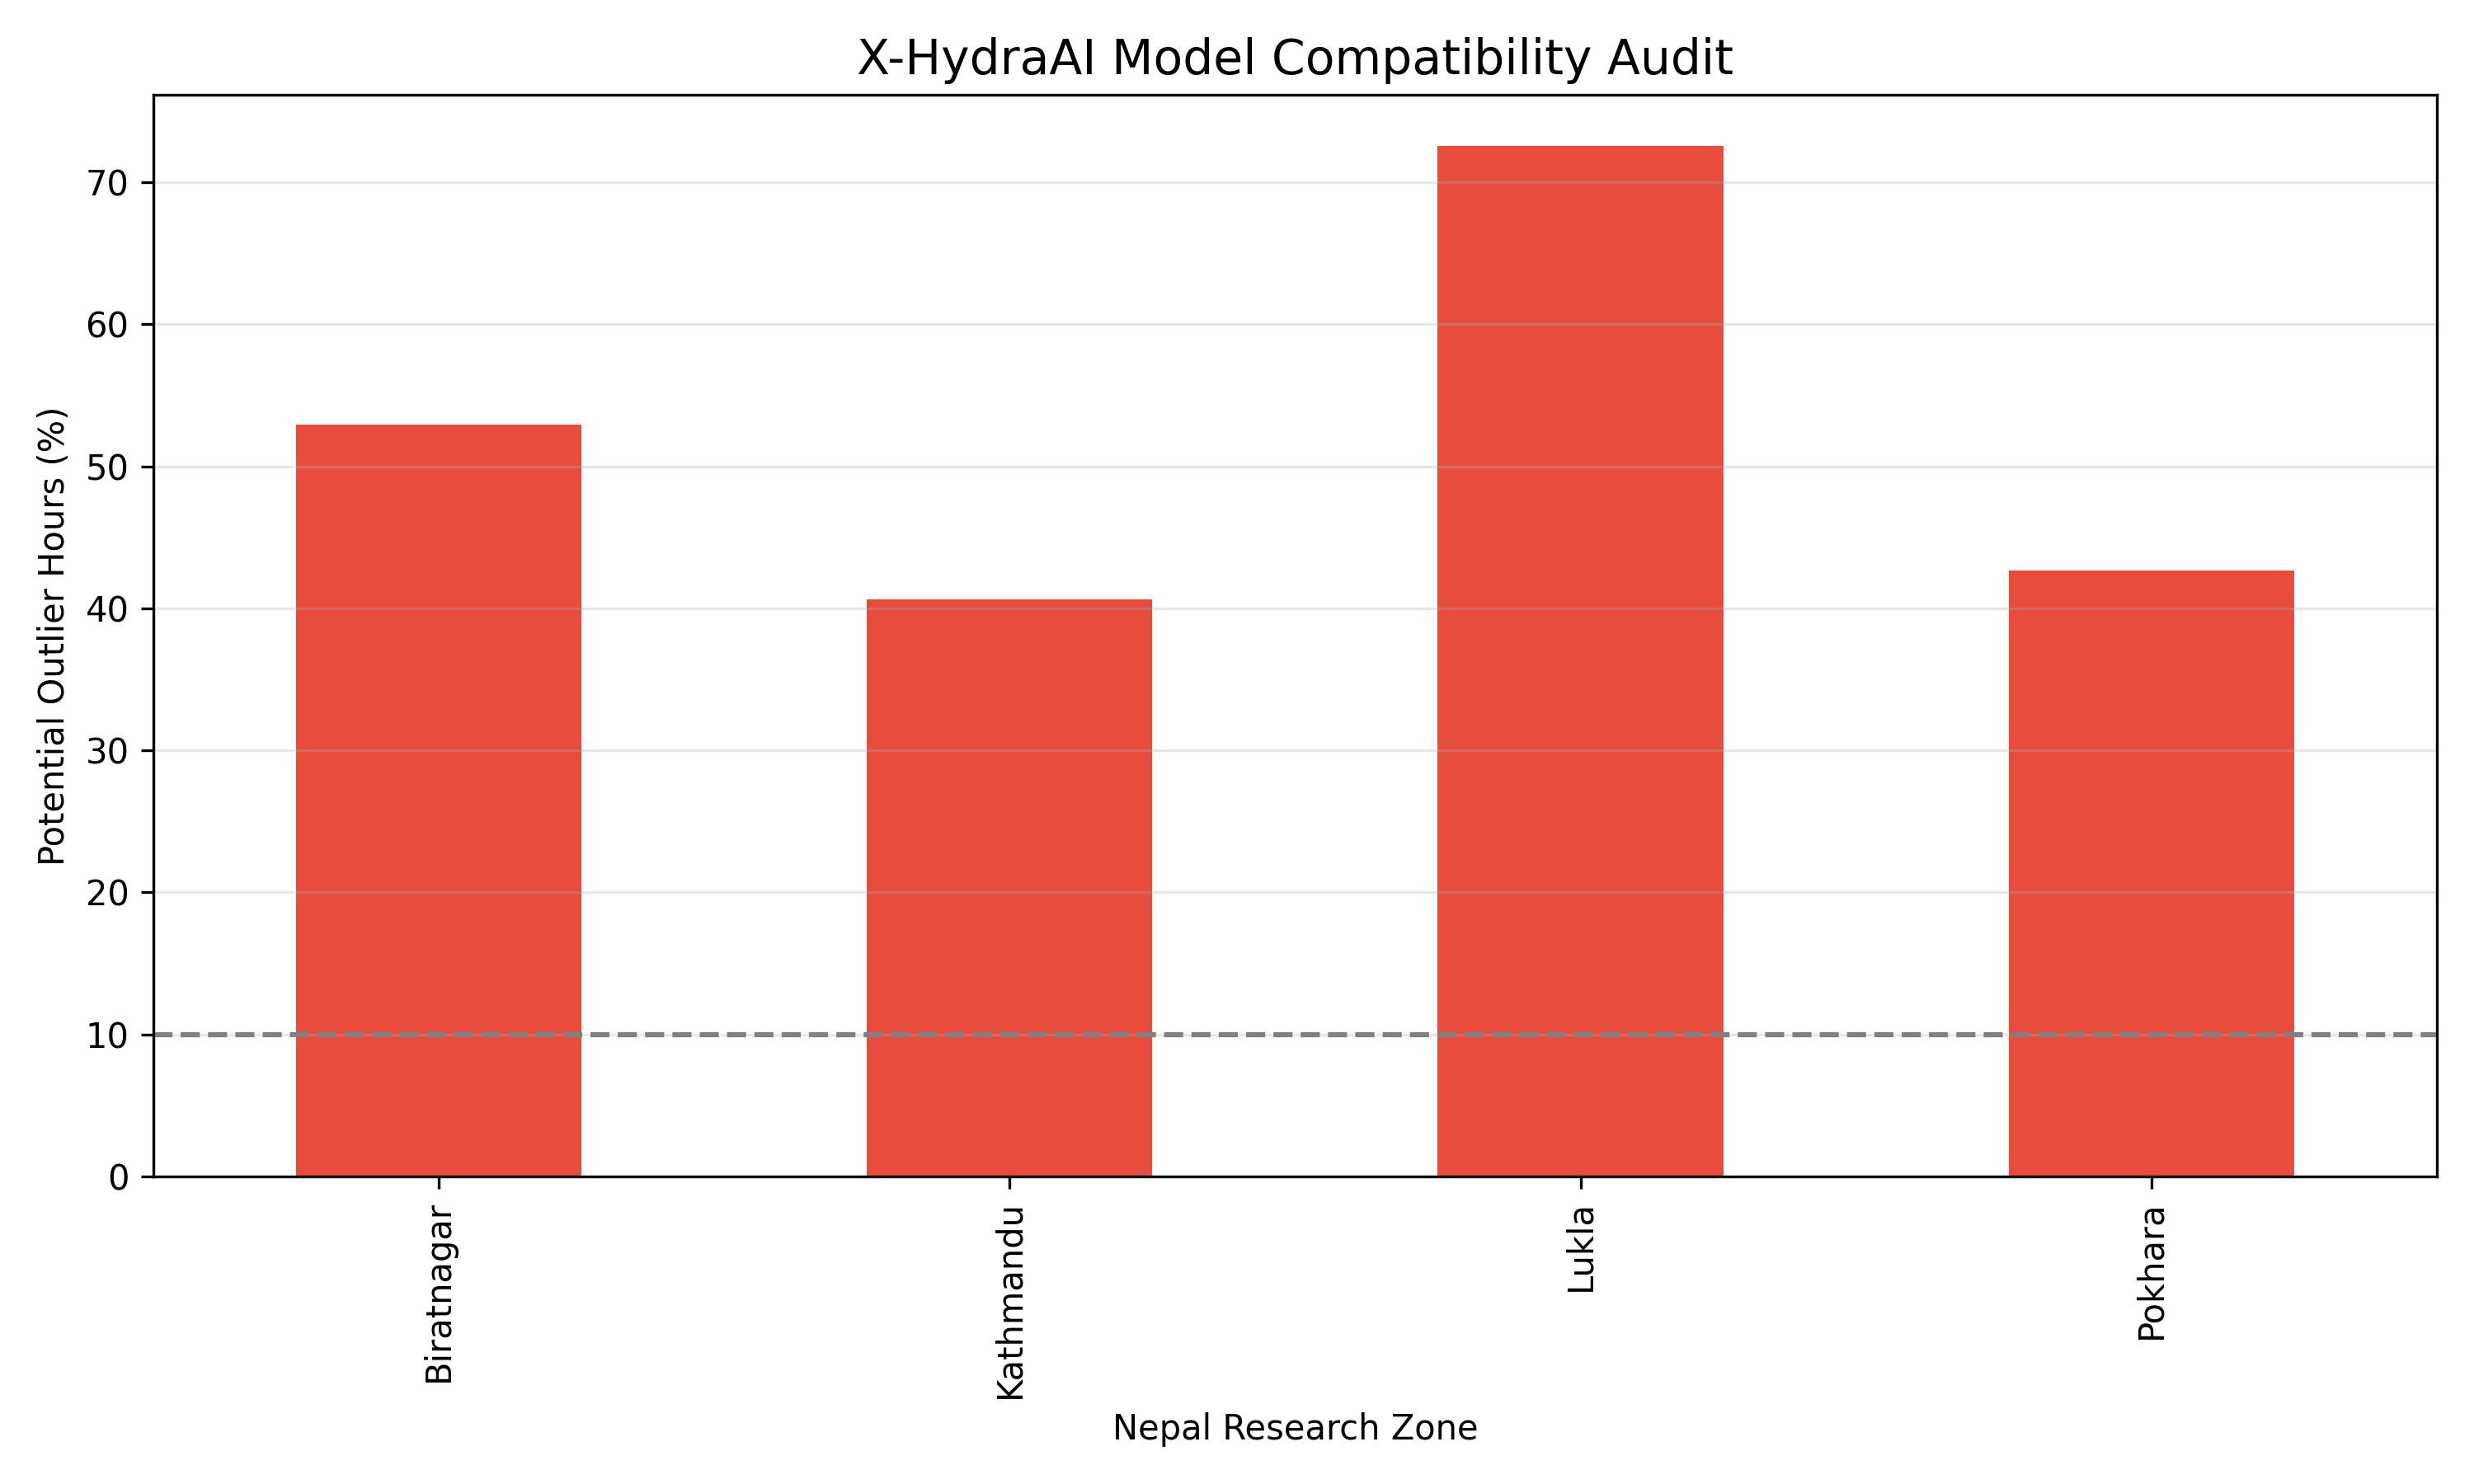
\includegraphics[width=\textwidth]{nepal_anomaly_audit.png}
    \caption{Nepal Anomaly Audit}
\end{minipage}
\end{figure}

\begin{figure}[H]
\centering
\begin{minipage}{0.45\columnwidth}
    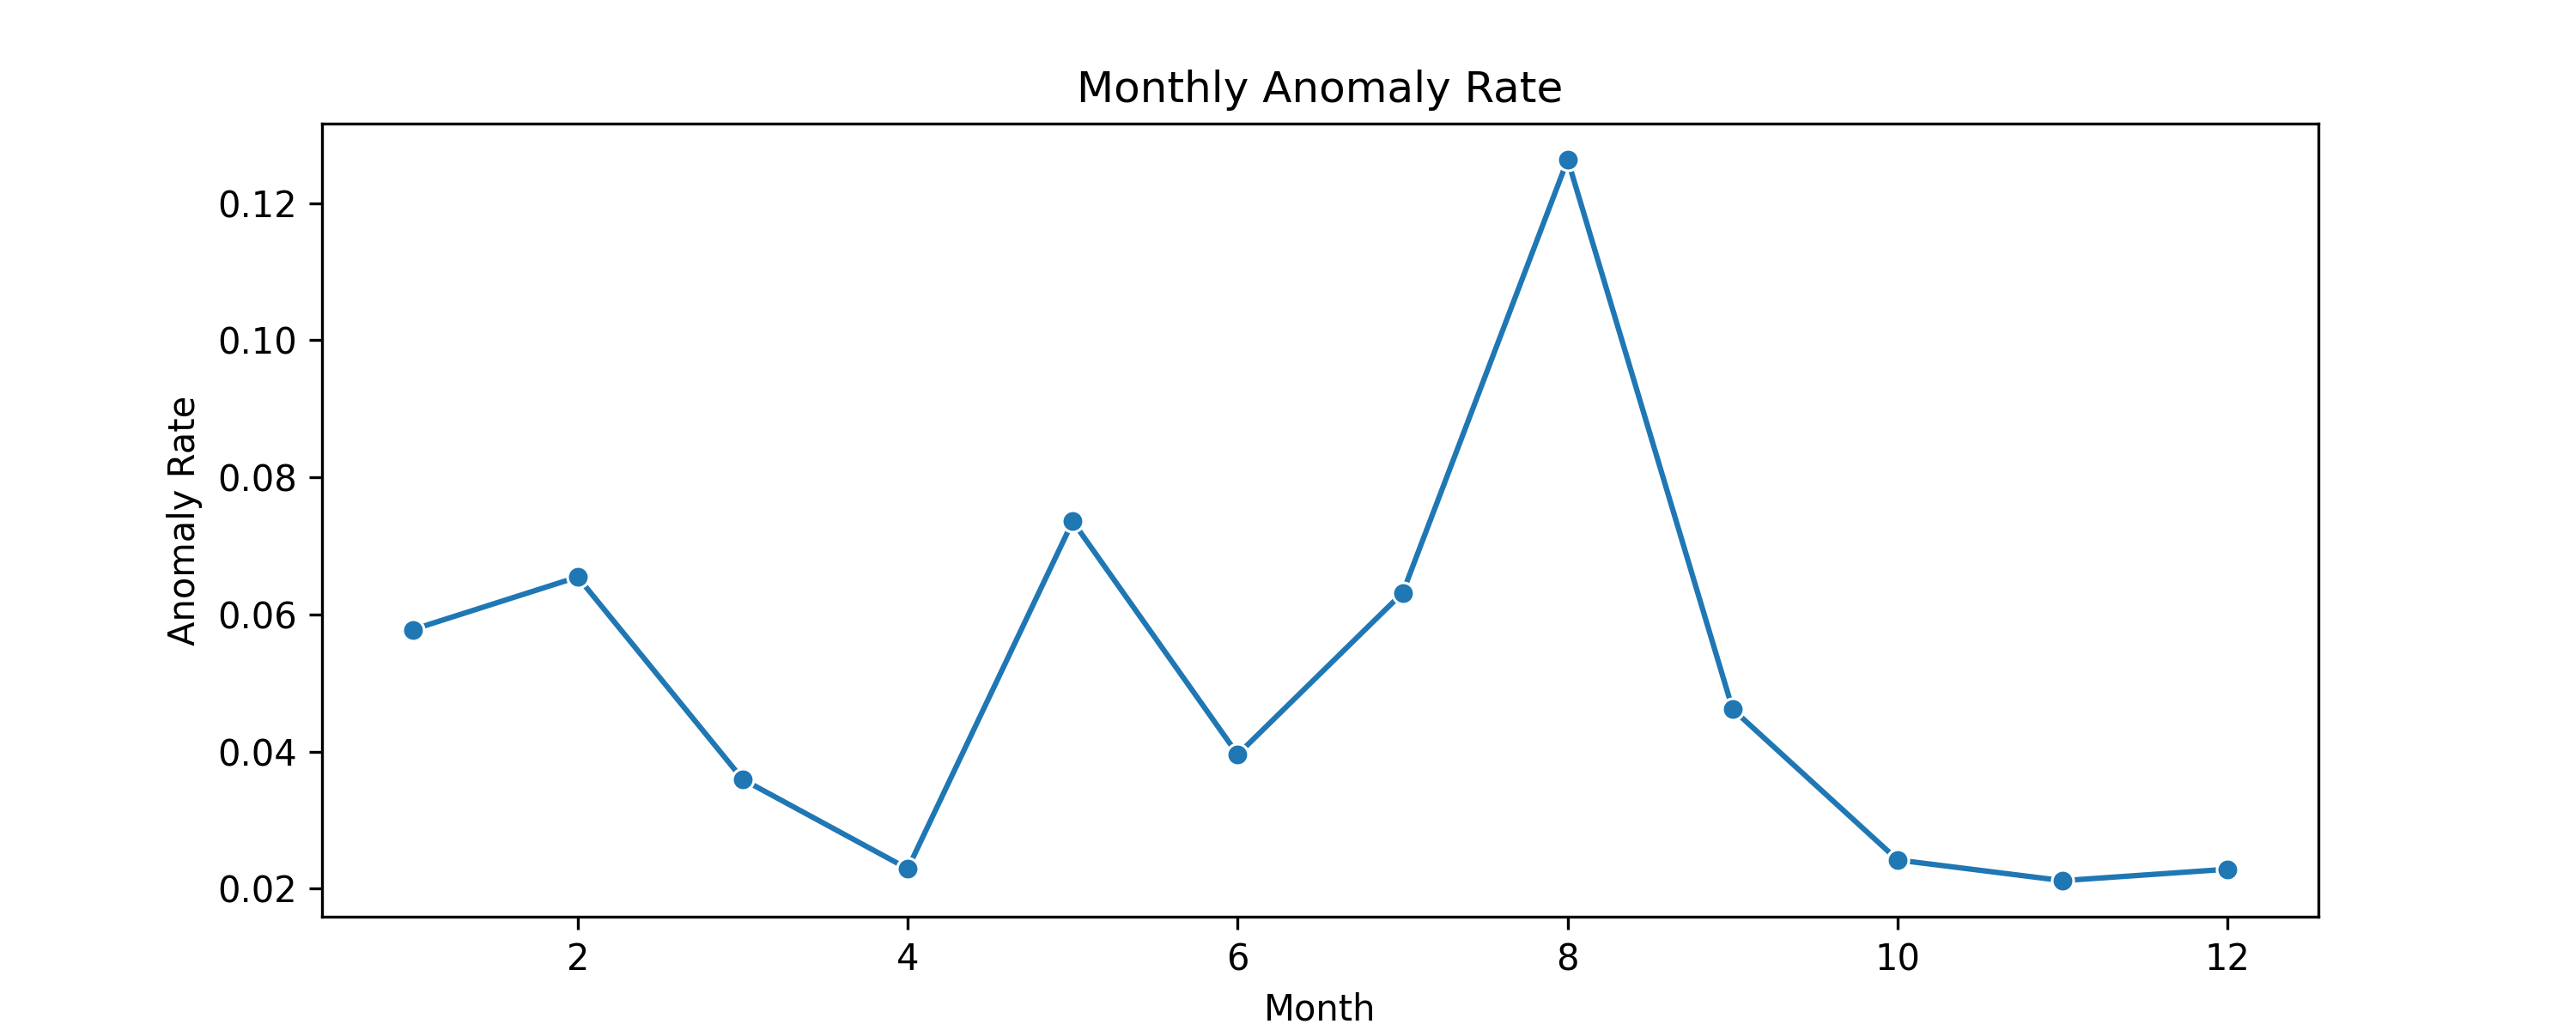
\includegraphics[width=\textwidth]{monthly_anomaly_trend.png}
    \caption{Monthly Anomaly Trend}
\end{minipage}
\hfill
\begin{minipage}{0.45\columnwidth}
    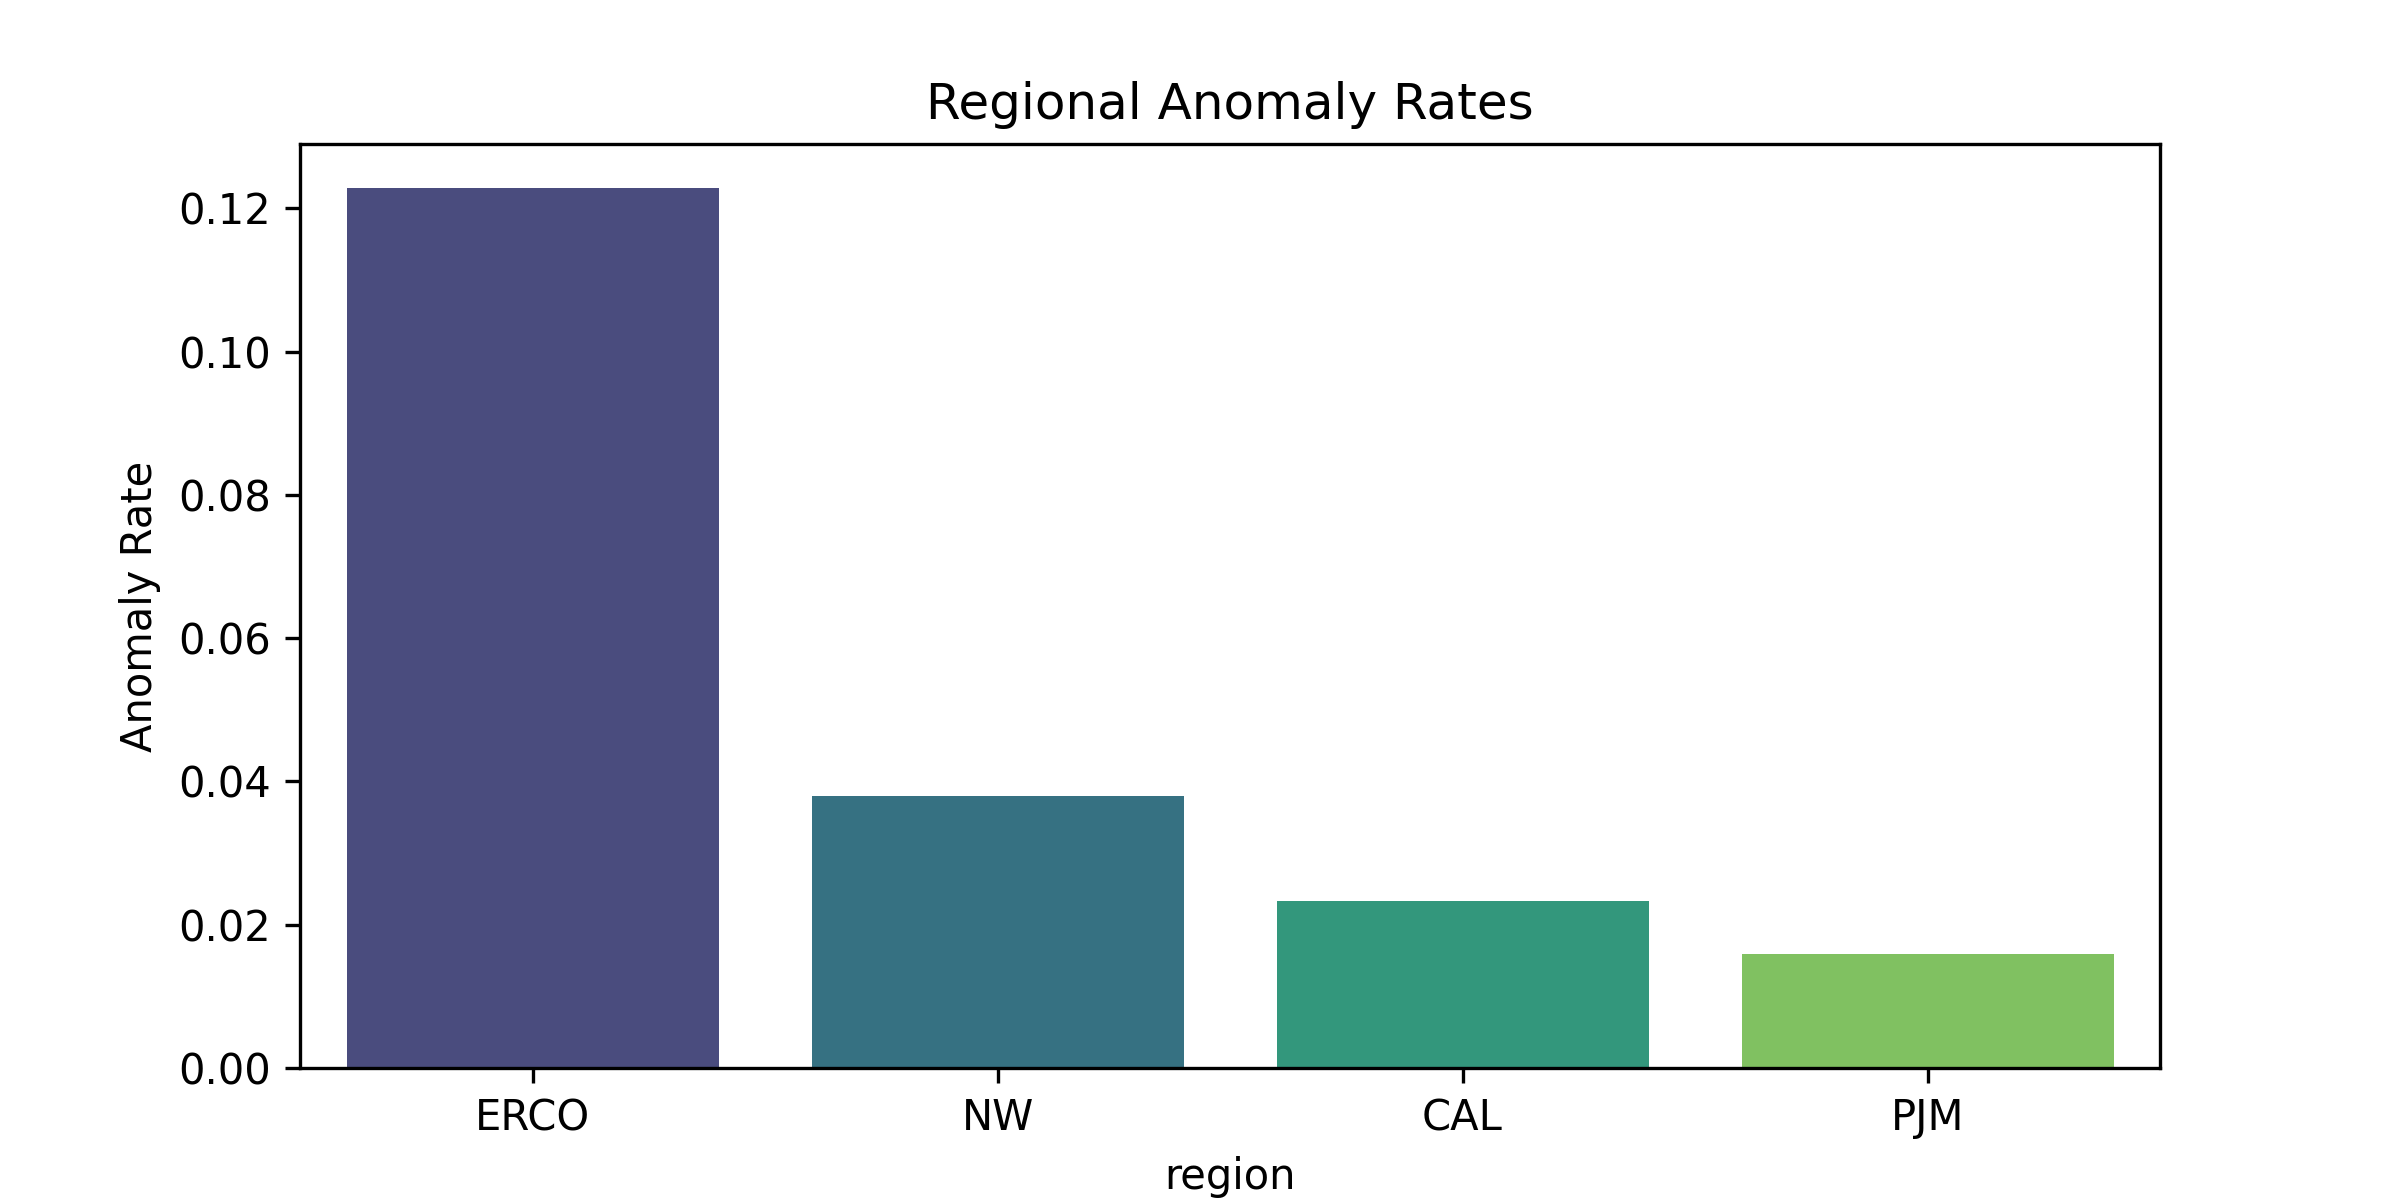
\includegraphics[width=\textwidth]{regional_anomaly_rates.png}
    \caption{Regional Anomaly Rates}
\end{minipage}
\end{figure}

\begin{figure}[H]
\centering
\begin{minipage}{0.45\columnwidth}
    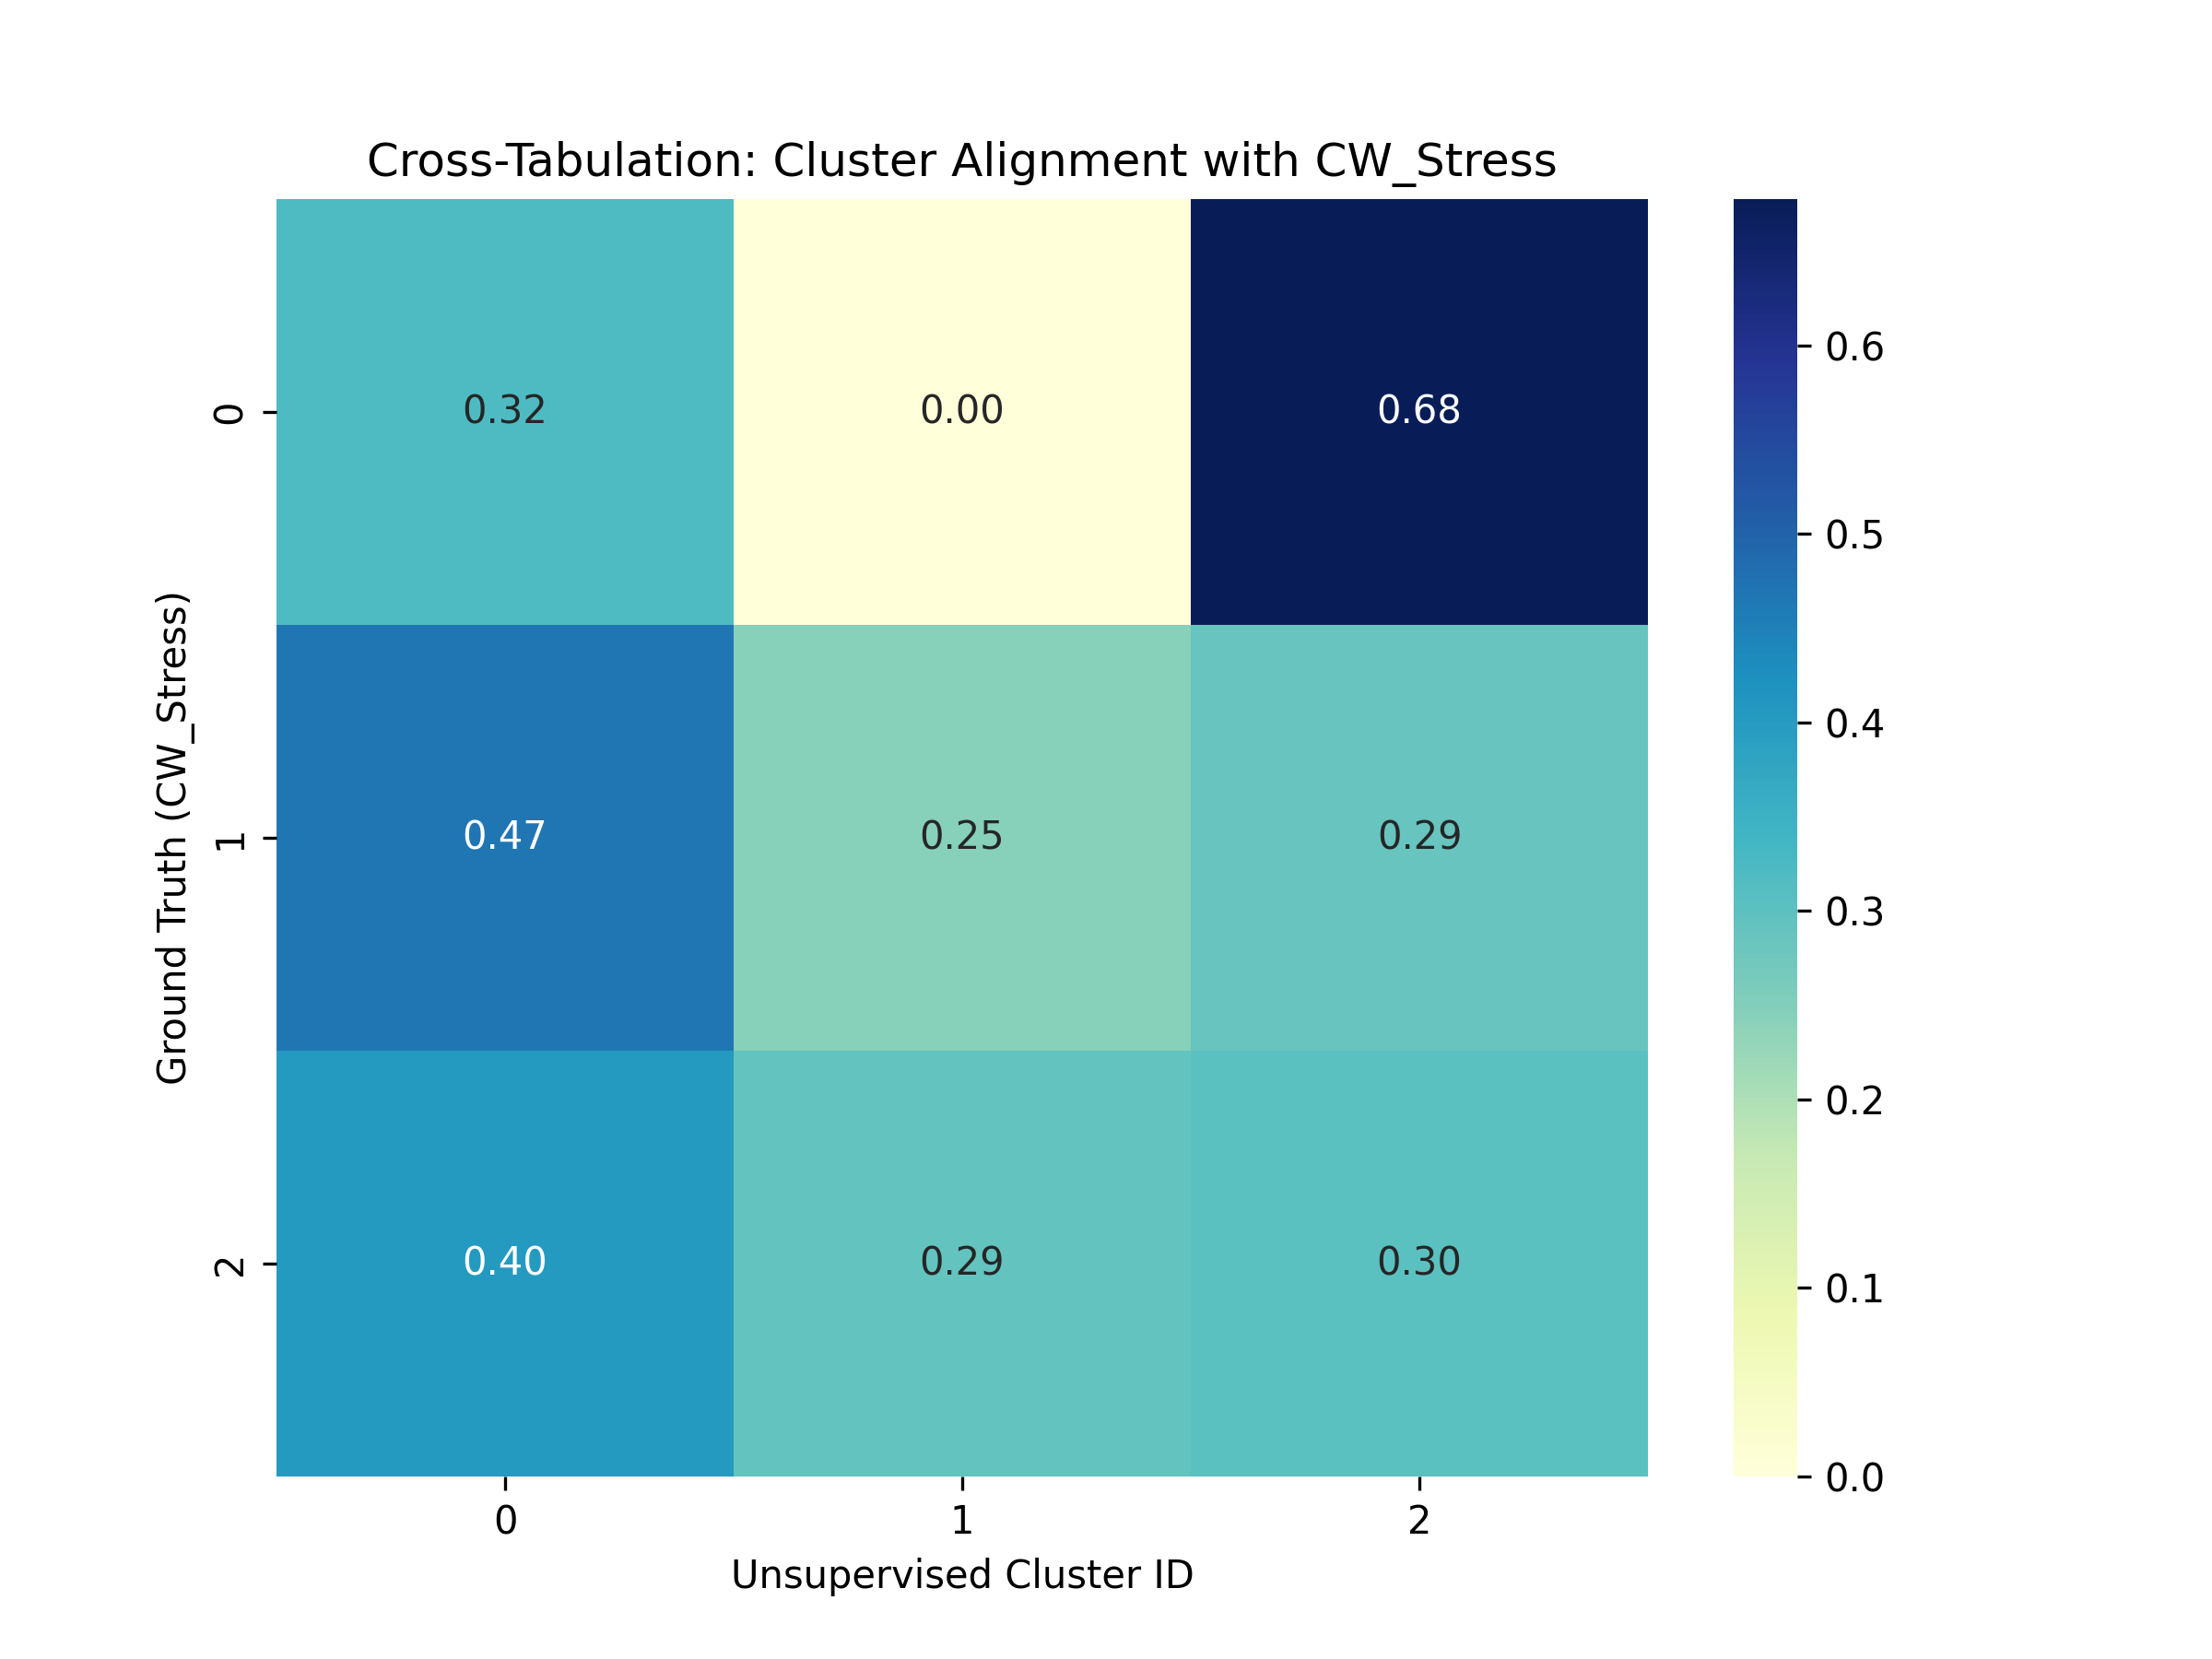
\includegraphics[width=\textwidth]{clustering_crosstab.png}
    \caption{Cluster Alignment Audit}
\end{minipage}
\hfill
\begin{minipage}{0.45\columnwidth}
    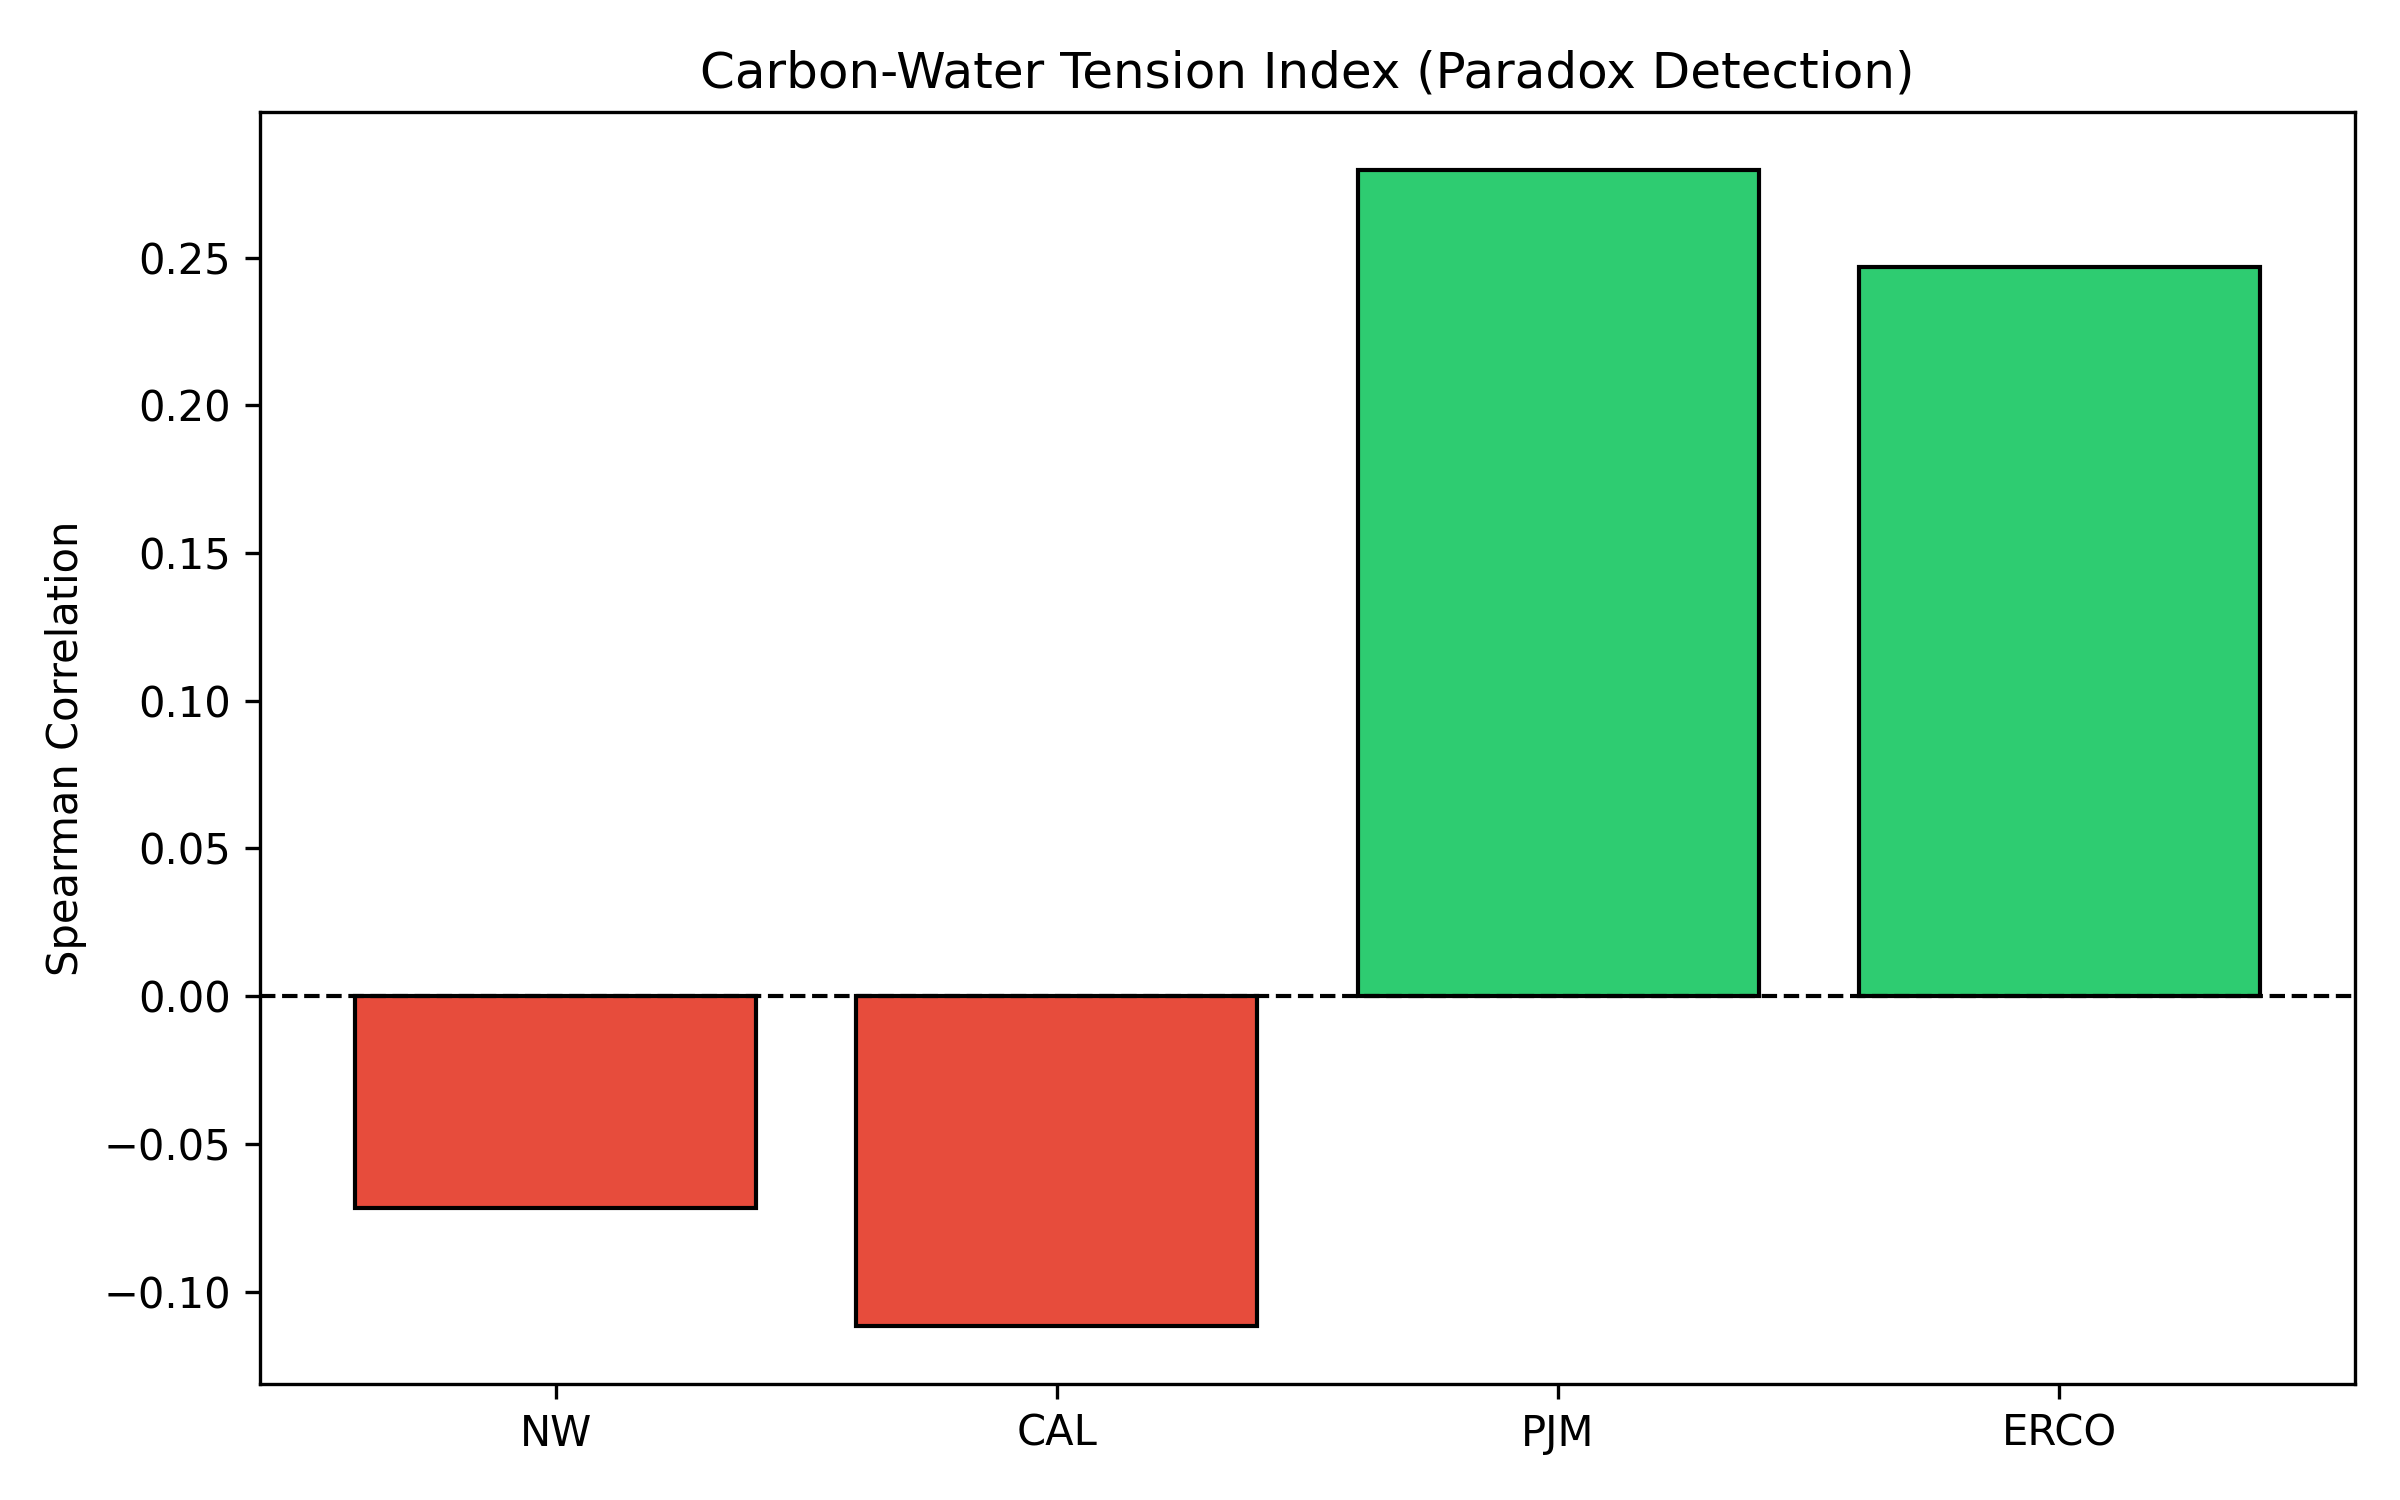
\includegraphics[width=\textwidth]{tension_index.png}
    \caption{Carbon-Water Tension}
\end{minipage}
\end{figure}

\begin{figure}[H]
\centerline{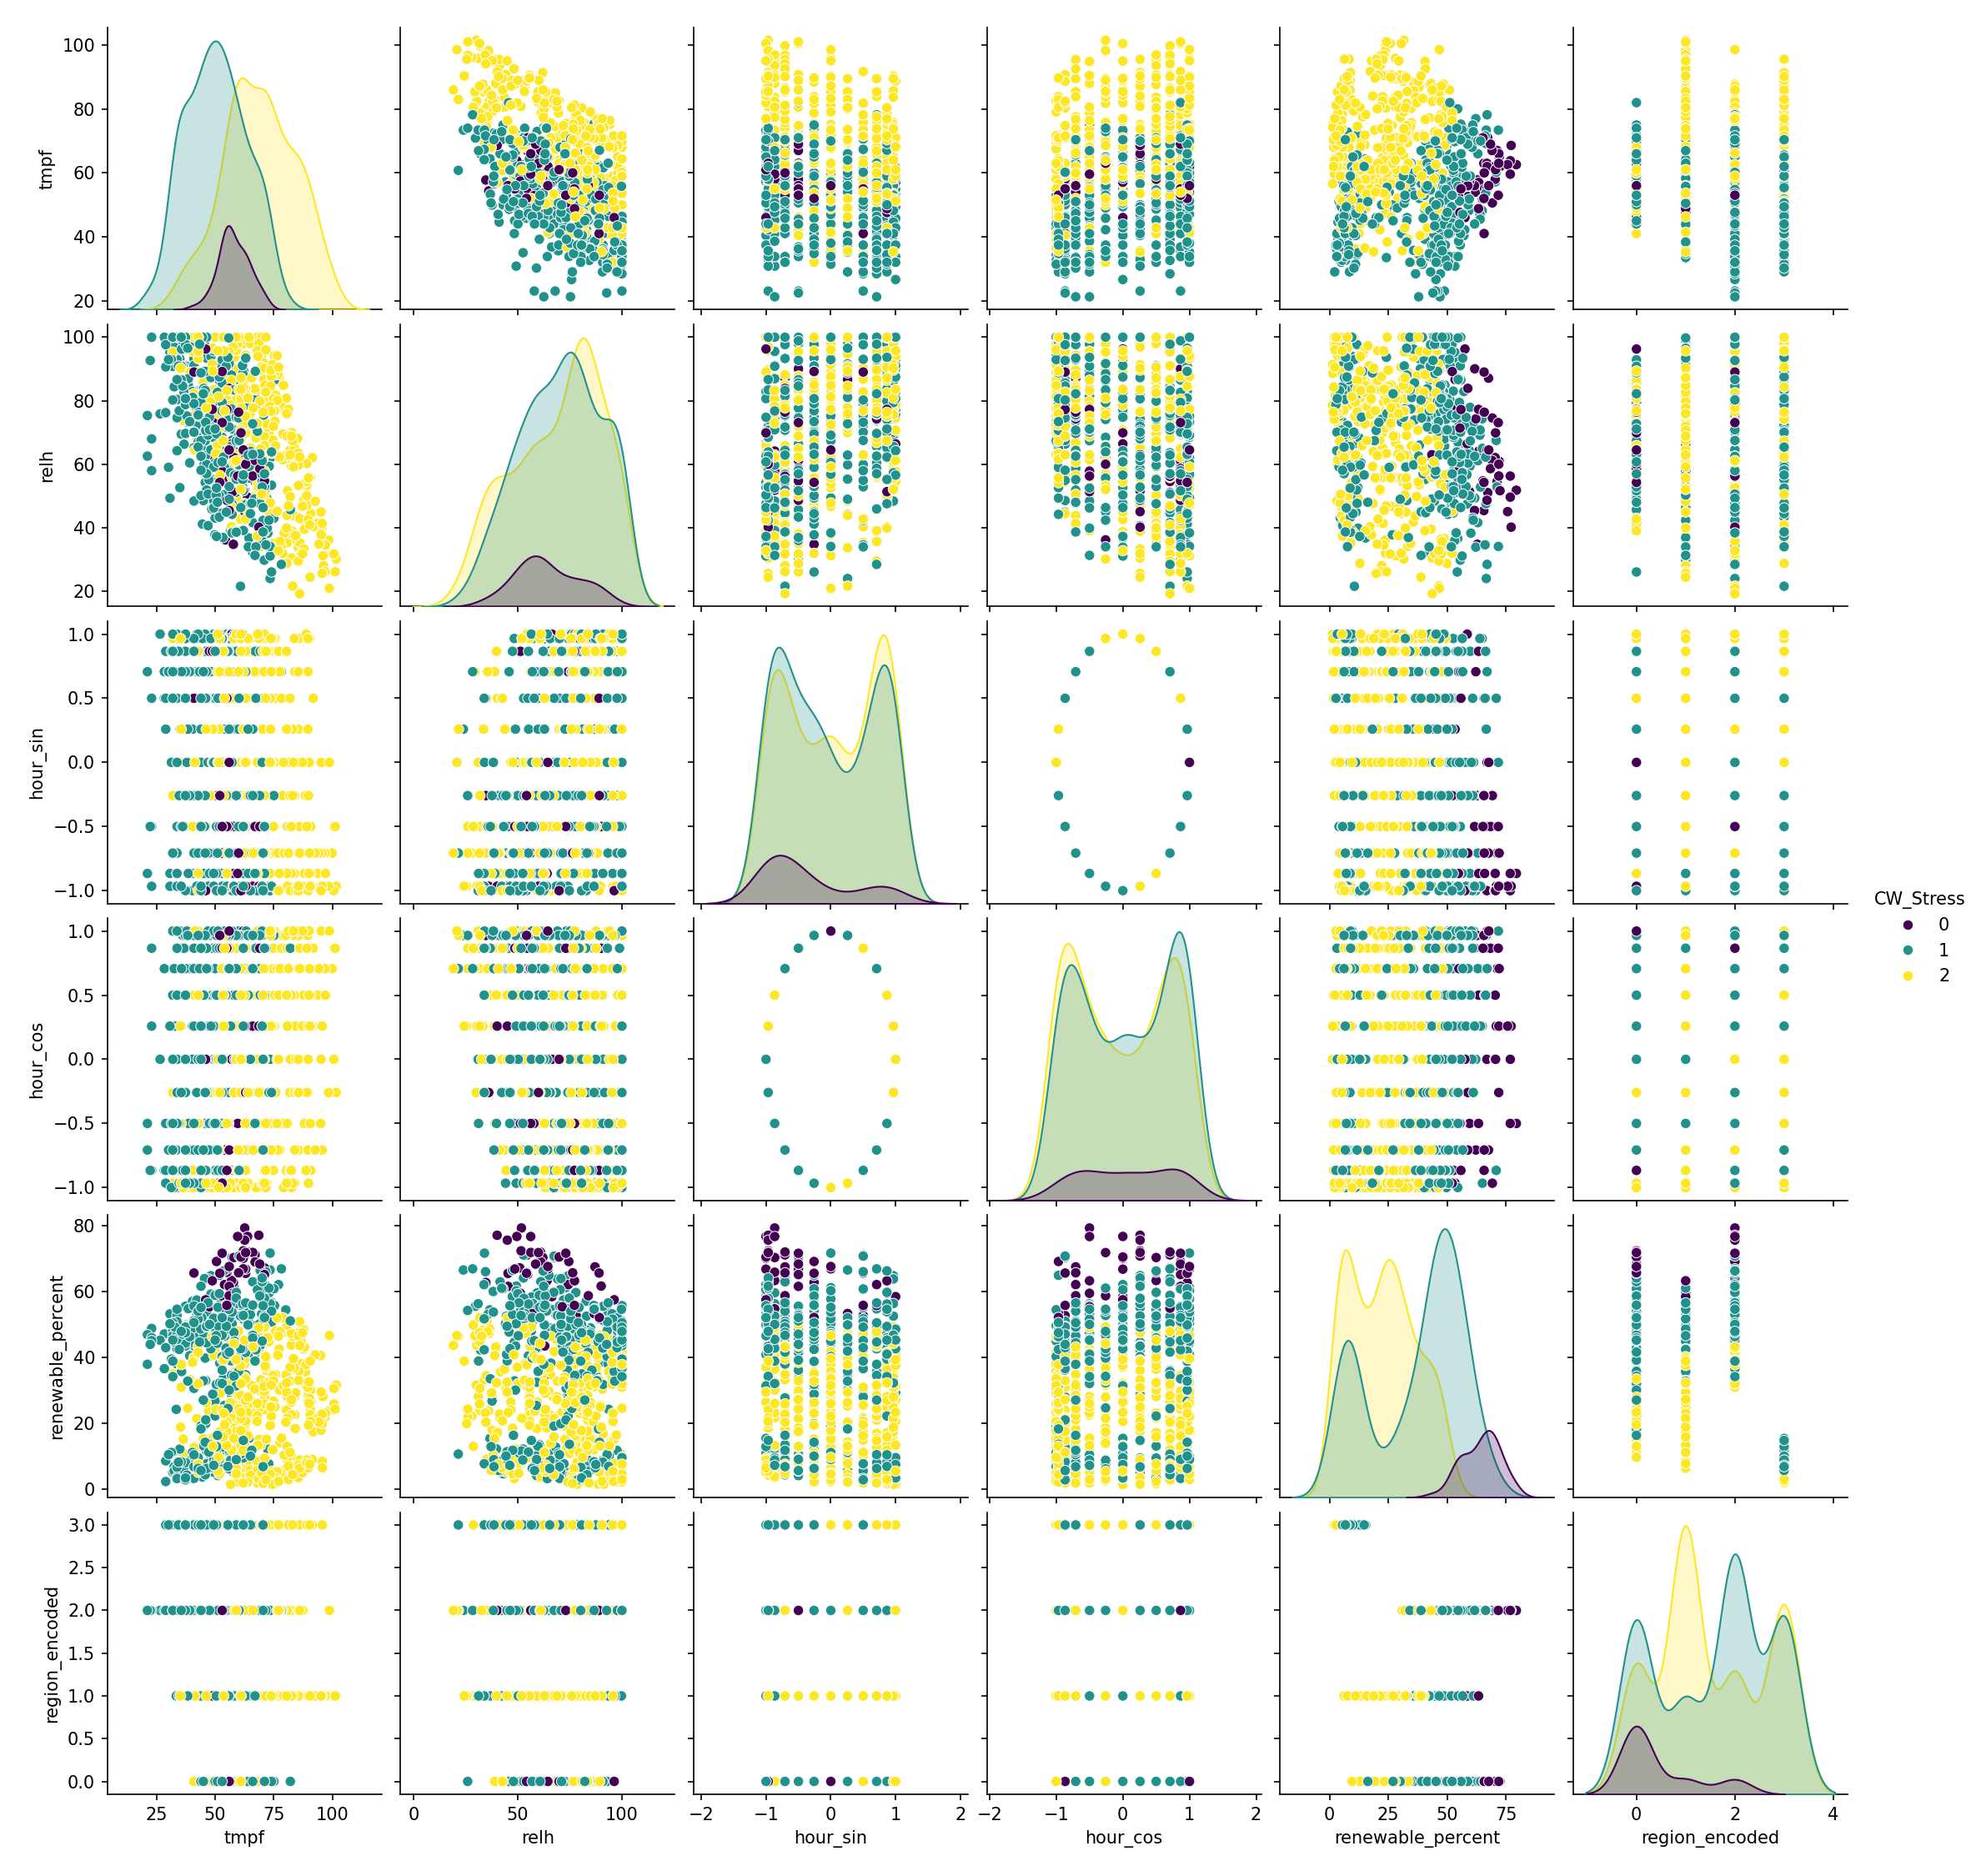
\includegraphics[width=0.9\columnwidth]{feature_pairplot.png}}
\caption{Global Feature Pairplot: High-dimensional interaction analysis of the 35,040-hour master dataset.}
\end{figure}

\begin{figure}[H]
\centering
\begin{minipage}{0.45\columnwidth}
    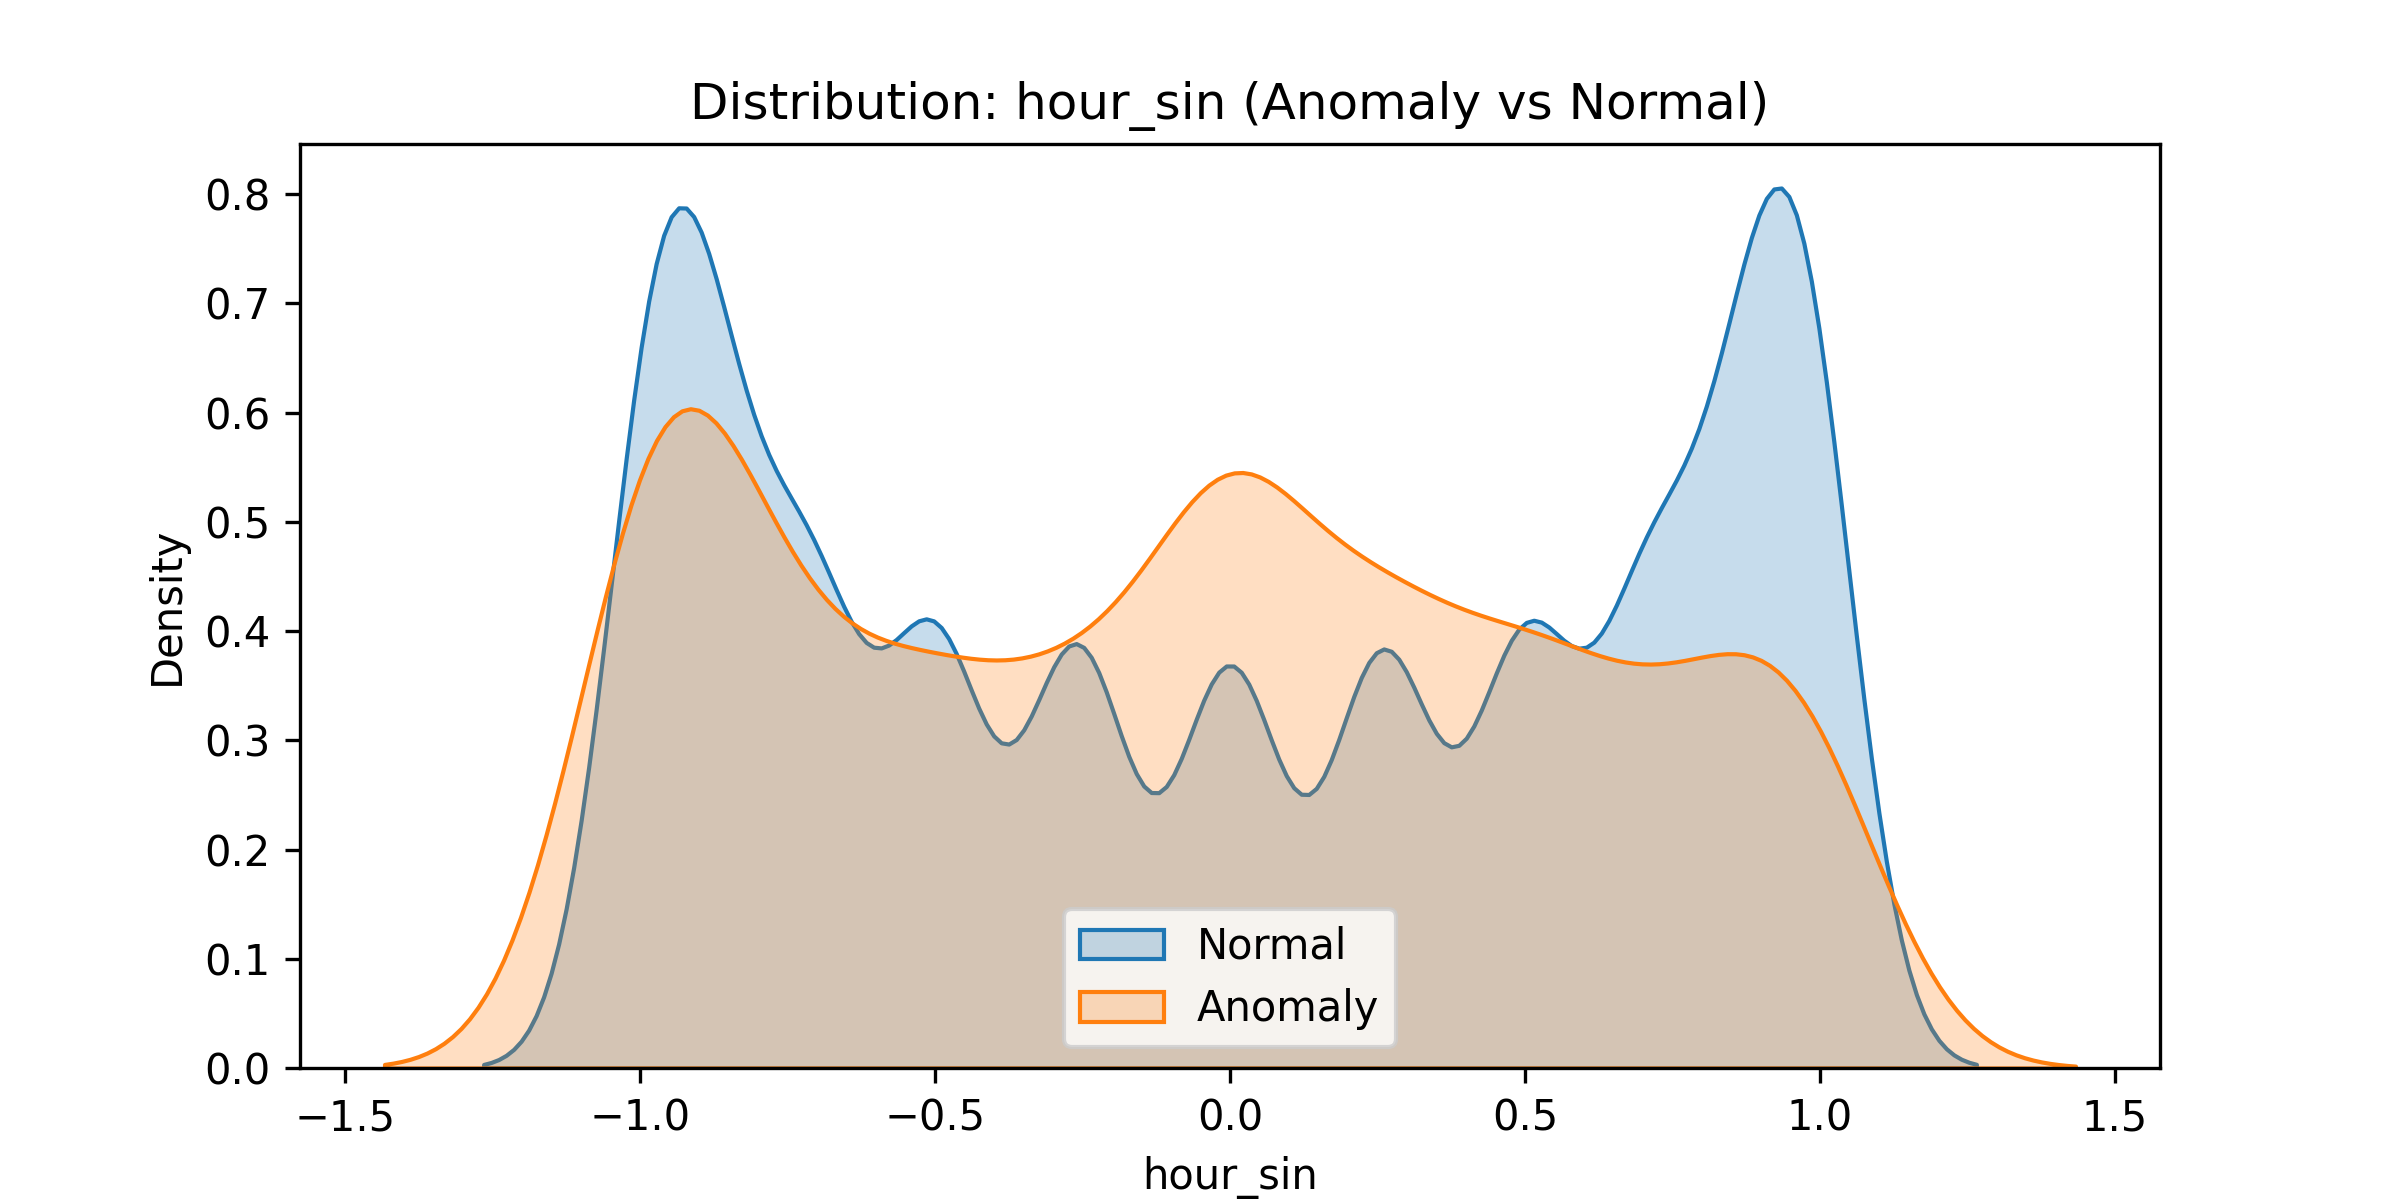
\includegraphics[width=\textwidth]{anomaly_dist_hour_sin.png}
    \caption{Temporal Anomaly Audit}
\end{minipage}
\hfill
\begin{minipage}{0.45\columnwidth}
    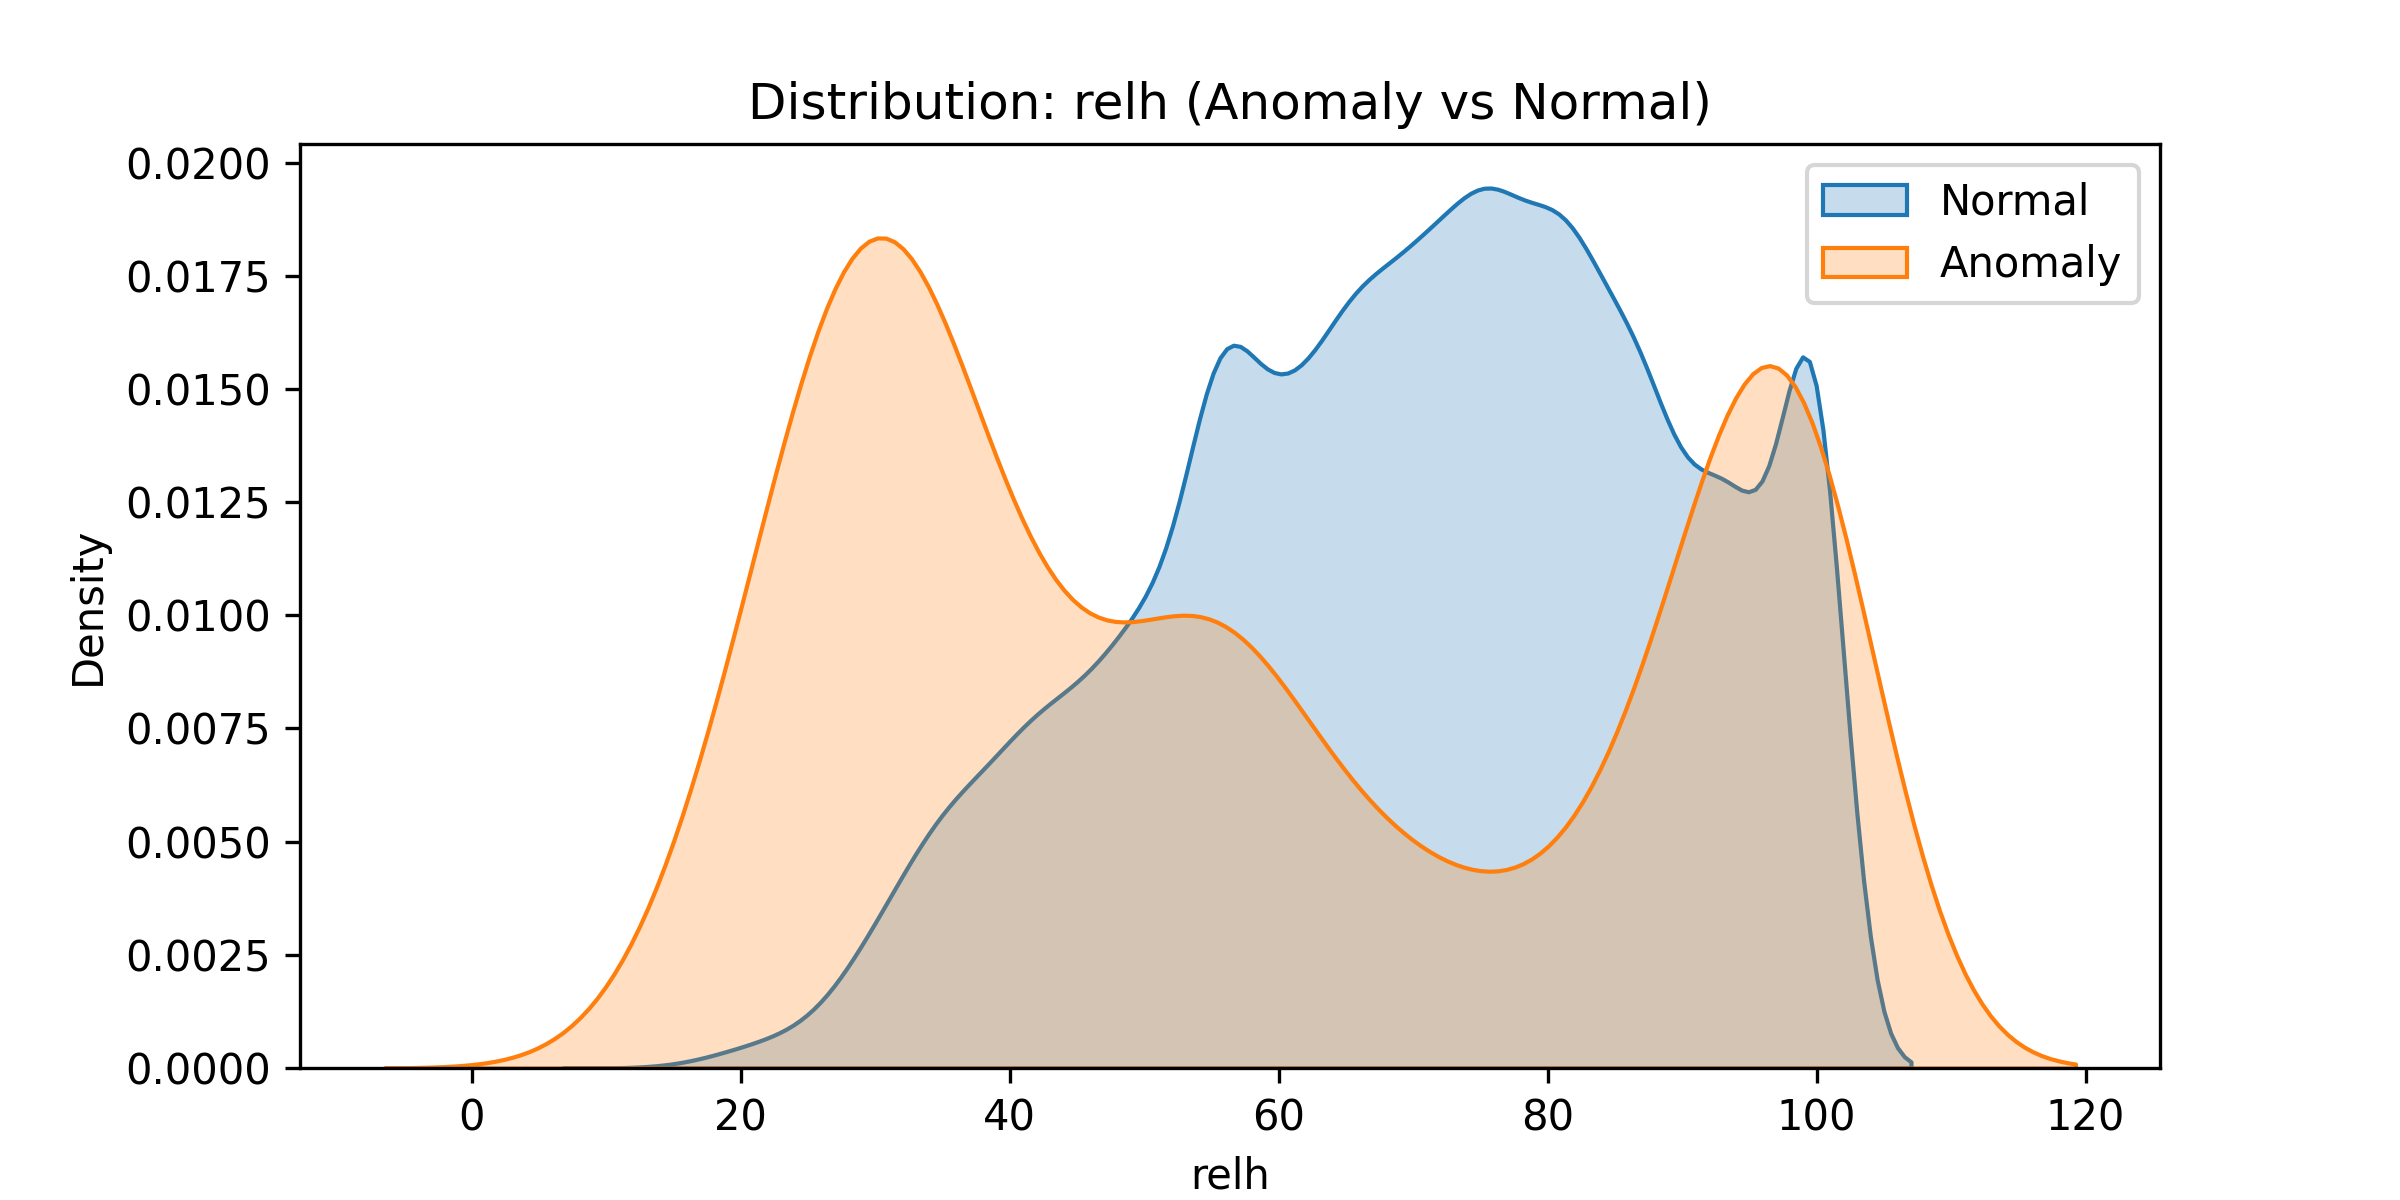
\includegraphics[width=\textwidth]{anomaly_dist_relh.png}
    \caption{Humidity Anomaly Audit}
\end{minipage}
\end{figure}

\begin{figure}[H]
\centering
\begin{minipage}{0.45\columnwidth}
    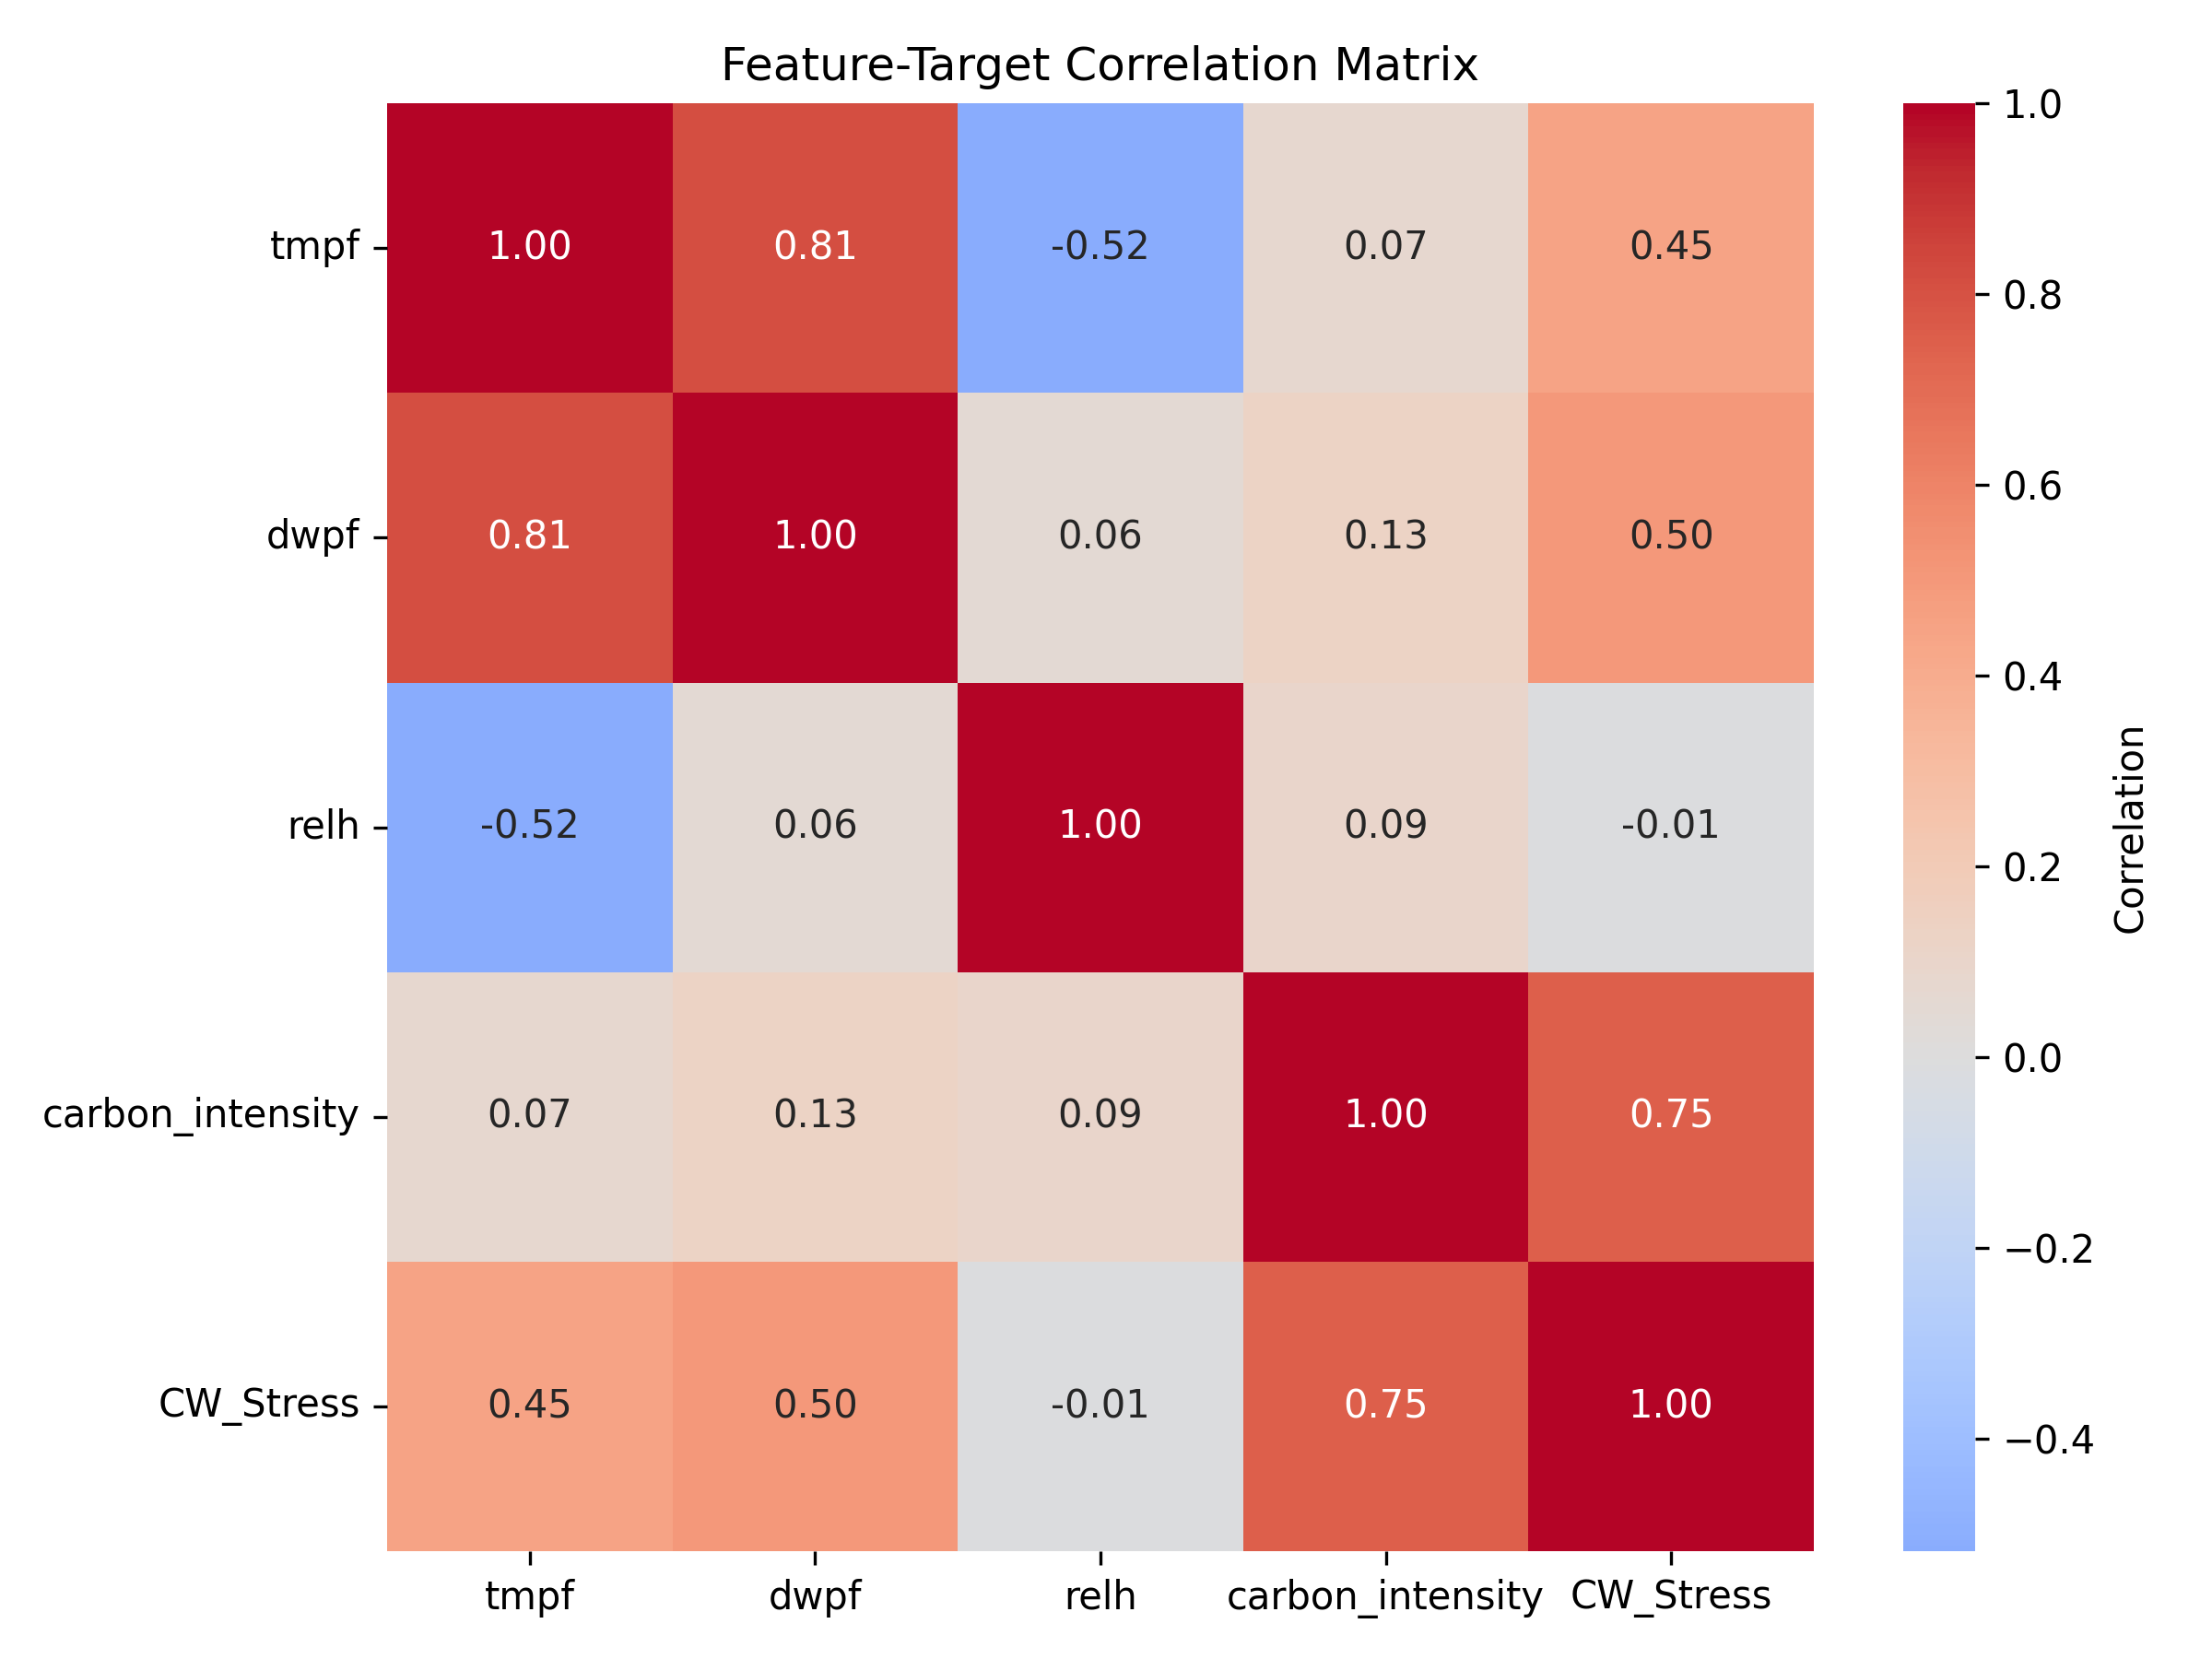
\includegraphics[width=\textwidth]{correlation_matrix.png}
    \caption{Secondary Correlation Matrix}
\end{minipage}
\hfill
\begin{minipage}{0.45\columnwidth}
    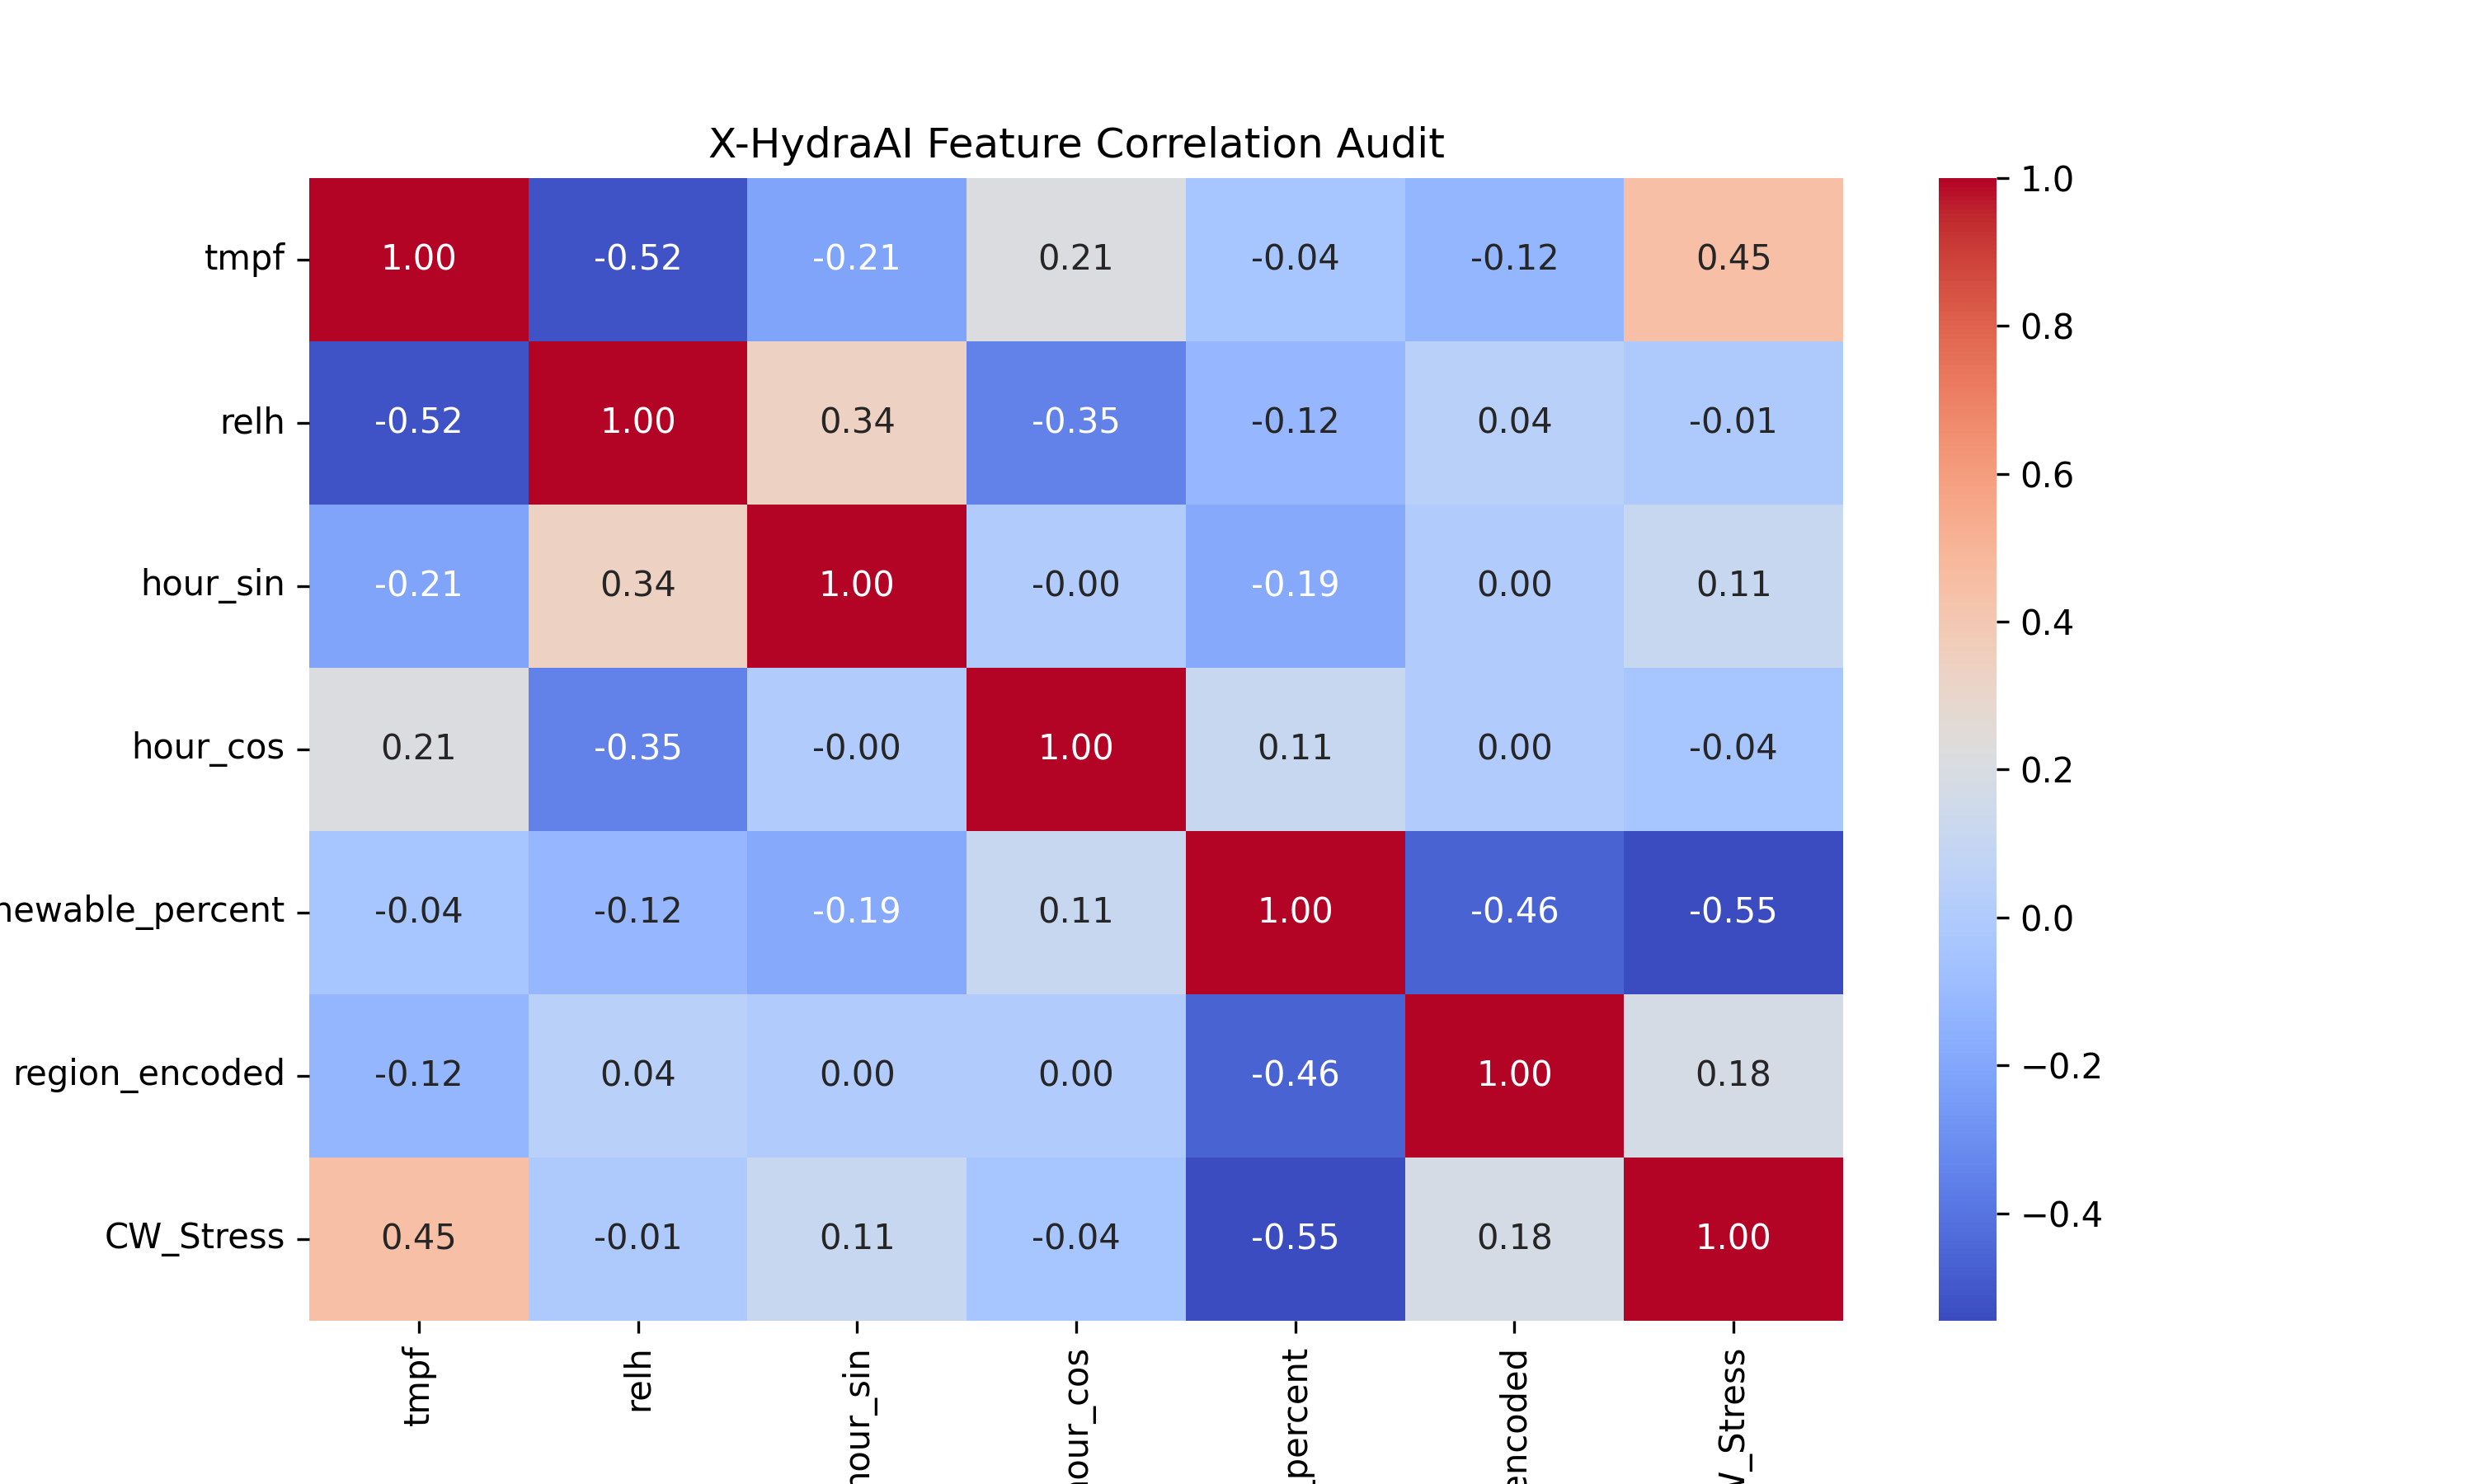
\includegraphics[width=\textwidth]{feature_correlation_audit.png}
    \caption{Feature Cross-Audit}
\end{minipage}
\end{figure}



\section*{REFERENCES}
\begin{thebibliography}{40}
\bibitem{b1} J. Masanet et al., ``Recalibrating global data center energy-use estimates,'' \textit{Science}, vol. 367, no. 6481, pp. 984–986, 2020.
\bibitem{b2} Goldman Sachs Research, ``Generative AI: The next productivity frontier,'' 2024. [Online].
\bibitem{b3} D. Patterson et al., ``Carbon Emissions and Large Neural Network Training,'' \textit{arXiv:2104.10350}, 2021.
\bibitem{b4} Google, ``Our carbon-intelligent computing platform,'' \textit{Google Research Blog}, 2020.
\bibitem{b5} The Green Grid, ``Water Usage Effectiveness (WUE): A Real-Time Metric for Data Center Efficiency,'' White Paper \#35, 2021.
\bibitem{b6} B. Dodge et al., ``Measuring the Carbon Intensity of AI in Cloud Instances,'' \textit{FAccT '22}, pp. 1877–1894, 2022.
\bibitem{b7} P. Li et al., ``Making AI Less 'Thirsty': Uncovering the Environmental Footprint of AI Models,'' \textit{arXiv:2304.03271}, 2023.
\bibitem{b8} S. Ahmad et al., ``Machine learning for data center energy efficiency: A systematic review,'' \textit{Energy and AI}, vol. 15, p. 100321, 2024.
\bibitem{b9} S. M. Lundberg and S. I. Lee, ``A Unified Approach to Interpreting Model Predictions,'' \textit{NeurIPS}, 2017.
\bibitem{b10} IPCC, ``Climate Change 2022: Mitigation of Climate Change,'' \textit{AR6}, 2022.
\bibitem{b11} R. Stull, ``Wet-bulb temperature from relative humidity and air temperature,'' \textit{J. Appl. Meteor. Climatol.}, vol. 50, pp. 2267–2269, 2011.
\bibitem{b12} A. Radovanovic et al., ``Carbon-Aware Computing for Data Centers,'' \textit{IEEE Transactions on Sustainable Computing}, 2021.
\bibitem{b13} IEA, ``Electricity 2025: Analysis and forecast to 2027,'' International Energy Agency, 2025.
\bibitem{b14} ASHRAE, ``Standard 90.4-2022: Energy Standard for Data Centers,'' 2022.
\bibitem{b15} U.S. EIA, ``Hourly Real-Time Fuel Mix Data,'' \textit{EIA API v2}, 2023. [Online].
\bibitem{b16} Iowa State University, ``Iowa Environmental Mesonet: ASOS/AWOS Hourly Weather Data,'' 2023. [Online].
\bibitem{b17} DHM Nepal, ``Climate Normals of Nepal (1991–2020),'' Department of Hydrology and Meteorology, 2023.
\bibitem{b18} F. T. Liu et al., ``Isolation Forest,'' \textit{ICDM '08}, pp. 413–422, 2008.
\bibitem{b19} N. V. Chawla et al., ``SMOTE: Synthetic Minority Over-sampling Technique,'' \textit{JAIR}, vol. 16, pp. 321–357, 2002.
\bibitem{b20} F. Pedregosa et al., ``Scikit-learn: Machine Learning in Python,'' \textit{JMLR}, vol. 12, pp. 2825–2830, 2011.
\bibitem{b21} V. Vapnik, \textit{The Nature of Statistical Learning Theory}, Springer-Verlag, 1995.
\bibitem{b22} Joblib Development Team, ``Joblib: running Python functions as pipeline jobs,'' 2023. [Online].
\bibitem{b23} Nepal Electricity Authority (NEA), ``Annual Report 2022/23,'' Kathmandu, Nepal, 2023.
\bibitem{b24} IEEE, ``Standard 7000-2021: Model Process for Addressing Ethical Concerns during System Design,'' 2021.
\bibitem{b25} L. Breiman, ``Random Forests,'' \textit{Machine Learning}, vol. 45, no. 1, pp. 5–32, 2001.
\bibitem{b26} Scikit-Learn, ``TimeSeriesSplit documentation,'' v1.3.2, 2023. [Online].
\bibitem{b27} Net Zero Tracker, ``Post-COP28 Analysis of Net Zero Targets,'' 2024. [Online].
\bibitem{b28} Carbon Aware Computing, ``Real-time carbon intensity APIs for scheduling,'' 2023. [Online].
\bibitem{b29} M. H. Siddik et al., ``The Environmental Footprint of Data Centers,'' \textit{Environmental Research Letters}, vol. 16, no. 6, 2021.
\bibitem{b30} C. Molnar, \textit{Interpretable Machine Learning: A Guide for Making Black Box Models Explainable}, 2022.
\bibitem{b31} R. Hyndman, ``Cross-validation for time series,'' \textit{Hyndsight}, 2016. [Online].
\bibitem{b32} P. Bholowalia, ``EBK-Means: A Clustering Technique based on Elbow Method,'' \textit{IJCA}, 2014.
\bibitem{b33} L. Hubert and P. Arabie, ``Comparing partitions,'' \textit{Journal of Classification}, vol. 2, pp. 193–218, 1985.
\bibitem{b34} L. Lacoste et al., ``Quantifying the Carbon Emissions of Machine Learning,'' \textit{arXiv:1910.02199}, 2019.
\bibitem{b35} P. J. Rousseeuw, ``Silhouettes: a graphical aid to the interpretation and validation of cluster analysis,'' \textit{J. Comp. Appl. Math.}, 1987.
\bibitem{b36} Government of Nepal, ``Digital Nepal Framework 2019,'' Ministry of Communication and Information Technology, 2019.
\bibitem{b37} IPCC, ``AR6 Synthesis Report: Climate Change 2023,'' 2023.
\bibitem{b38} ASHRAE, ``Liquid Cooling Guidelines for Datacom Equipment Centers,'' 2021.
\bibitem{b39} NEA, ``Cross-Border Electricity Trade Progress Report,'' Kathmandu, 2024.
\bibitem{b40} B. K. Sovacool et al., ``The social justice of low-carbon energy transitions,'' \textit{Energy Policy}, 2021.
\end{thebibliography}

\end{document}
